\documentclass[b5paper, twoside, titlepage, 11pt]{article}

% Så sier vi fra om hvilke tilleggspakker vi trenger
% til dokumentet vårt. De som du ikke trenger (se kommentaren) 
% kan det være en fordel å kommentere ut (sett prosenttegn foran),
% da vil kompilering gå raskere.

%\usepackage[norsk]{babel}	% norske navn rundt omkring
\usepackage[T1]{fontenc}		% norsk tegnsett (æøå)
\usepackage[utf8]{inputenc}	% norsk tegnsett
\usepackage[b5paper]{geometry}		% anbefalt pakke for å styre marger.

\usepackage{amsmath,amsfonts,amssymb} % matematikksymboler
\usepackage{mathtools}
\usepackage{amsthm}                   % for å lage teoremer og lignende.
\usepackage{graphicx}                 % inkludering av grafikk
\usepackage{subcaption}                 % hvis du vil kunne ha flere
                                      % figurer inni en figur
\usepackage{listings}                 % Fin for inkludering av kildekode
\usepackage{setspace}
\usepackage{parskip}
\usepackage{placeins}                 % Floatbarrier
\usepackage[dvipsnames,svgnames]{xcolor}                   % Textcolor
\usepackage{hyperref}                 % Hyperlinks
\usepackage[round]{natbib}
\bibliographystyle{dcuurl}
\usepackage{booktabs}                 % Tables
\usepackage{tabularx, ragged2e}                 % Tables
\newcolumntype{C}{>{\Centering}X}    % centered version of X column type
\newcolumntype{L}{>{\RaggedRight\arraybackslash}X}  % ragged-right version of X col. type
\renewcommand\tabularxcolumn[1]{m{#1}}% for vertical centering text in X column

\usepackage[inkscapearea=page]{svg}
%\usepackage{caption}
%\usepackage{subcaption}

%\usepackage{natbib}                   % Bibliography management
\usepackage{titlesec}
\usepackage{hyperref}
\usepackage{tikz}
\usepackage{titlesec}
\usepackage[htt]{hyphenat}
\usepackage{url}

\mathtoolsset{showonlyrefs}

\titleclass{\subsubsubsection}{straight}[\subsection]

\newcounter{subsubsubsection}[subsubsection]
\renewcommand\thesubsubsubsection{\thesubsubsection.\arabic{subsubsubsection}}
\renewcommand\theparagraph{\thesubsubsubsection.\arabic{paragraph}} % optional; useful if paragraphs are to be numbered

\titleformat{\subsubsubsection}
  {\normalfont\normalsize\bfseries}{\thesubsubsubsection}{1em}{}
\titlespacing*{\subsubsubsection}
{0pt}{3.25ex plus 1ex minus .2ex}{1.5ex plus .2ex}

\makeatletter
\renewcommand\paragraph{\@startsection{paragraph}{5}{\z@}%
  {3.25ex \@plus1ex \@minus.2ex}%
  {-1em}%
  {\normalfont\normalsize\bfseries}}
\renewcommand\subparagraph{\@startsection{subparagraph}{6}{\parindent}%
  {3.25ex \@plus1ex \@minus .2ex}%
  {-1em}%
  {\normalfont\normalsize\bfseries}}

  \def\toclevel@subsubsubsection{4}
\def\toclevel@paragraph{5}
\def\toclevel@paragraph{6}
\def\l@subsubsubsection{\@dottedtocline{4}{7em}{4em}}
\def\l@paragraph{\@dottedtocline{5}{10em}{5em}}
\def\l@subparagraph{\@dottedtocline{6}{14em}{6em}}
\makeatother

\setcounter{secnumdepth}{4}
\setcounter{tocdepth}{4}

\numberwithin{equation}{section}
\counterwithin{figure}{section}

\captionsetup[subfigure]{font={bf,large}, skip=1pt, margin=0cm, singlelinecheck=false}



\setlength{\parindent}{0pt}           % Set indents to zero
\usepackage{enumitem}
\renewcommand{\theenumi}{\alph{enumi}}
\usepackage{listings}

\lstset{language=R,
    basicstyle=\small\ttfamily,
    stringstyle=\color{DarkGreen},
    otherkeywords={0,1,2,3,4,5,6,7,8,9},
    morekeywords={TRUE,FALSE},
    deletekeywords={data,frame,length,as,character, weights, by, formula, scale, family, log, list, control},
    keywordstyle=\color{blue},
    commentstyle=\color{DarkGreen},
}

\renewcommand{\contentsname}{Table of Contents}
\linespread{1.22}
\begin{document}

% På forsida skal vi ikke ha noen sidenummerering:

\pagestyle{empty}
\pagenumbering{roman}

% Inkluder forsida:
\newcommand\myemptypage{
    \null
    \thispagestyle{empty}
    \addtocounter{page}{-1}
    \newpage
    } %sets new page command to insert an empty page without adding to the page counter or having a page number

\begin{titlepage}
    \newgeometry{left=1.6in, right=2in}
    \begin{figure}[h]
        \includegraphics[width=\textwidth]{Figures/NTNU-Bred.pdf}
    \end{figure}
    \vspace*{1.5cm}
    
    \noindent \textbf{\LARGE Education-Specific Differences in Time Trends of Age-Stratified Back Pain Data of US Adults from 1997 to 2018} \\

    \vspace*{-0.4cm}
    \noindent {\large A multivariate age-period-cohort analysis} \\
    \vspace{0.5cm}

    \noindent  \textcolor{gray}{\Large Markus Trætli} \\
    \vspace{0.5cm}
    
    
    \vspace{1.5cm}%For a4: 7cm, For b5:3.5-3.7 
    \noindent Master's thesis in Mathematics \\
    Supervisor: Andrea Riebler \\
    Co-supervisor: Ingeborg Hem Sørmoen \\
    Submission date: June 2024 \\
    
    \vspace{0.2cm}
    \noindent Norwegian University of Science and Technology \\
    Faculty of Information Technology and Electrical Engineering \\
    Department of Mathematical Sciences \\
\end{titlepage}
\restoregeometry
\myemptypage %empty page such that the abstract starts at the first right hand side after the title page
%\end{comment}

% Local Variables:
% TeX-master: "master"
% End:


% Romerske tall på alt før selve rapporten starter er pent.
\pagenumbering{roman}

% For å ikke begynne innholdslista på baksida av forsida:
\cleardoublepage
% (kun aktuelt når man har twoside som global opsjon)

% Nå vi vil ha noe i topp- og bunnteksten
\pagestyle{headings}
\titleformat{\section}[block]{\normalfont\fontsize{20}{25}\bfseries\filcenter}{}{1em}{}
\section*{Abstract}
Chronic back pain is a globally prevalent health problem, compromising the general and psychological health of affected individuals, alongside economic consequences on both personal and societal levels. Back pain is found to be more prominent among adults with lower educational attainment, and the disparities between educational groups are suspected to be wider in more recent birth cohorts.

In this thesis, Bayesian multivariate age-period-cohort models are used to analyse temporal trends along age, period, and birth cohorts in chronic back pain in United States adults, stratified by the level of attained education. The data, taken from the National Health Interview Survey in the period 1997 to 2018, focuses on adults aged 25 to 84, and they are categorized into four educational groups. Smoothing priors are used to stabilize the estimates of the time trends, with joint hyperpriors elicited using expert knowledge provided by a sociologist. The complex survey design is accounted for using a recently-proposed two-step approach. For completeness, our analysis also includes model selection procedures, prior sensitivity analysis, and further investigations of subpopulations.

We found strong disparities in back pain trends over age and birth cohorts in all levels of attained education compared to the level "bachelor or above". Particularly strong disparities were identified for the "less than high school" and "general educational development" educational groups. The trends over age increased noticeably between ages 25 and 60, and then decreased afterwards. Moreover, the back pain disparities were also confirmed to have a distinct increase with more recent cohorts. Overall, the approach used to account for the survey design proved effective, and is recommended in future applications of age-period-cohort models.


\cleardoublepage
\newpage
\section*{Sammendrag}
Kroniske ryggsmerter er et globalt utbredt helseproblem som påvirker den generelle og psykologiske helsen til de berørte individene, med økonomiske konsekvenser på både personlig og samfunnsmessig nivå. Forskning har funnet at ryggsmerter er mer fremtredende blant voksne med lavere oppnådd utdanning, og forskjellene mellom utdanningsgrupper mistenkes å være større i nyere fødselskohorter.

I denne oppgaven brukes Bayesianske multivariate alder-periode-kohort-modeller til å analysere tidsmessige trender i ryggsmerter over alder, perioder og fødselskohorter hos voksne i USA, stratifisert etter nivå på oppnådd utdanning. Dataene, hentet fra National Health Interview Survey i perioden 1997 til 2018, omhandler voksne i alderen 25 til 84 år, kategorisert i fire utdanningsgrupper. Utjevningspriorifordelinger brukes til å stabilisere estimatene av tidstrendene, med hyperpriorifordelinger dannet ved hjelp av ekspertkunnskap supplert av en sosiolog. Det komplekse undersøkelsesdesignet er gjort rede for ved hjelp av en nylig foreslått to-trinns metode. For fullstendighetens skyld inkluderer analysen vår også modellvalgprosedyrer, sensitivitetsanalyse av priorifordelingene og videre undersøkelser av underpopulasjoner.

Vi fant sterke forskjeller i ryggsmertetrender over alder og fødselskohorter på alle nivåer av oppnådd utdanning sammenlignet med nivået "bachelor or above". Spesielt store forskjeller ble identifisert for utdanningsgruppene "less than high school" og "general educational development". Trendene over alder ser ut til å øke mellom 25 og 60 år, og avtar deretter. I tillegg ble det bekreftet at ulikhetene i ryggsmerte også økte med nyere kohorter. I det hele viste det seg at metoden som ble brukt for å redegjøre for undersøkelsesdesignet var effektiv, og den anbefales dermed i fremtidige anvendelser av alder-periode-kohort-modeller.

\cleardoublepage
\newpage
\section*{Preface}
This thesis is the result of my work in the course \textit{TMA4900 Industrial
Mathematics, Master’s Thesis} at the Norwegian University of Science and
Technology (NTNU), concluding my Master’s degree in Applied Physics and Mathematics at NTNU, specializing in Industrial Mathematics. I extend my greatest thanks to my supervisor Andrea Riebler, as well as my co-supervisor Ingeborg Hem Sørmoen for their excellent guidance, support and encouragement. 

I thank Anna Zajacova (Professor of Sociology, Western University) and Snehalata V. Huzurbazar (Acting Professor of Statistics, Emory University) for starting this project and letting me be part of it. Thank you for the fruitful discussions and comments. Thank you, Anna, for providing me with your sociological expert knowledge regarding backpain which allowed me to investigate prior elicitation as part of this thesis. 

Furthermore, I would also like to thank my fellow students for making my journey at NTNU truly memorable. Finally, I thank my family and Connie for their unwavering support and encouragement in these trying times.

\vspace{1cm}
\begin{flushleft}
    Markus Trætli\par
    June 2024\par
    Trondheim
\end{flushleft}
\cleardoublepage
\newpage

% Si til LaTeX at vi vil ha ei innholdsliste generert akkurat her:
\linespread{0.7}
\tableofcontents
\linespread{1.25}
% Pass på at neste side ikke begynner på baksida av en annen side.
\cleardoublepage

% Arabisk (vanlige tall) sidenummerering. Starter på side 1 igjen.
\pagenumbering{arabic}

%Title format
\titleformat{\section}[block]{\normalfont\fontsize{15}{20}\bfseries\filcenter}{\thesection.}{1em}{}

\titleformat{\subsubsubsection}
  {\itshape\normalsize}{\thesubsubsubsection}{1em}{}

\section{Introduction}
\label{section:Introduction}
%Chronic pain, what is it, how common, how does it affect people
Chronic pain is one of the most common health conditions plaguing the general population, compromising the general and psychological health of the affected individuals \citep{becker1997pain, gureje1998persistent}, and in turn, influencing their social and economic well-being due to their reduced productive functioning \citep{latham1994socioeconomic}. Chronic pain is commonly defined as pain that persists past the healing phase following an injury \citep{merskey1986classification}. These conditions are typically labelled by site (e.g., back, head, viscera) and type (e.g., neuropathic, arthritic, cancer, myofascial, diabetic) \citep{APKARIAN200981} of injury. In personal and work life, chronic pain entails functional impairment leading to the inability to work and provide familial care. Coupled with the emotional distress that this condition may inflict, it is a key factor in quality of life and an enormous personal and economic burden \citep{duenas2016review}. The condition is estimated to have a high annual economic cost for society as a whole \citep{bp-cost}, with reported incidence rates in the United States up to $30\%$ \citep{johannes2010prevalence}. Despite the large societal burden of the condition, chronic pain has long gone unrecognized by international public health institutions, with the World Health Organization (WHO) finally representing the condition systematically in the 11th rendition International Classification of Diseases (ICD-11), which replaced the 10th rendition in 2022 \citep{ICD-11}. Considering the heavy burden caused by chronic pain, sociologists have consistently pushed for the condition to be recognized, all the while carrying out extensive research on the topic in recent decades \citep{gatchel2007biopsychosocial}. 

%Disparities in health by education, how and why
At the same time, in spite of extensive investigation on the biomedical, psychological and sociological aspects of chronic pain, questions regarding the trends in chronic pain remain unanswered. Among these questions lie the question of how trends in chronic pain have evolved over time, and how socioeconomic factors may have influenced these trends \citep{Zajacova2021-ee}. Education is one such factor, which has been investigated in several studies and is suggested as a powerful determinant of health \citep{mirowsky2017education}. Research has shown strong stratification in the health outcomes by level of attained education, with a lower prevalence of chronic conditions among individuals with higher levels of attained education \citep{dionne2001formal,kennedy2014prevalence}. In particular, recipients of the general educational development (GED) diploma, intended to be equivalent to a high school (HS) diploma, suffers from disproportionately worse health outcomes compared to individuals with higher attained education, such as bachelor's or master's degrees \citep{ZAJACOVA20201270}. The positive effect of education on health has been observed not only for chronic conditions, but also for other health conditions, such as functional limitations, disabilities, depressive symptoms, and active life expectancy \citep{montez2012educational,lorant2003socioeconomic,schoeni2005persistent}. Chronic pain also has the potential to act as a barometer for general health and well-being in a population, further underscoring the importance of research on the temporal trends in chronic pain with stratification by education \citep{sociology}.

%NHIS data and complex survey design
Research in the field is typically carried out using survey data collected from the population by medical institutions, organizations, or governmental institutions. The leading source of survey data on health in the United States is the National Health Interview Survey (NHIS) \citep{NHIS-original}. The NHIS is an ongoing cross-sectional household study in the United States collecting monthly samples on the general health of the civilian, non-institutionalized population. The design of the survey ensures that each monthly sample is nationally representative. Each year, approximately $50,000$ samples are collected, covering different topics such as health habits and conditions, as well as topics in relation to socioeconomic factors, including education and income. Among the covered topics in health is chronic pain, in which several categories of pain are represented. As such, the NHIS rightfully constitutes the basis for a lot of research related to chronic pain. An issue in using this data, however, is caused by the complexity introduced by survey design. Since the survey design of the NHIS is multistaged and makes use of geographically clustered sampling techniques, the estimates derived from models using their data may arrive at poor conclusions. In addition to the design, the NHIS has, in several years, oversampled some subpopulations (e.g., Black, Hispanic, Asian) to better assess the health of these groups. To produce correct statistical estimates, the NHIS provides sampling weights, which are used in statistical procedures to account for the design of the survey. Nonetheless, a lot of analyses neglect the potential importance of the survey design, though it should, in principle, always be accounted for.

%Age period cohort models
A prominent model in temporal analyses of health-related data is the age-period-cohort (APC) model. APC models have long been useful tools in the temporal analyses of health-related data, allowing for assessment of temporal trends of mortality, prevalence, and incidence rates by examining the data on three temporal scales \citep{APC-OLD, APC-OLD-2, APC-OLD-3}. Although the APC model was initially proposed in a frequentist framework using maximum likelihood methods for inference, Bayesian methods have become more frequent, incorporating a smoothing effect for each of the age, period and cohort effects \citep{APC-Bayesian-Yang, APC-Bayesian-Held}. Of particular interest in the Bayesian framework is the multivariate APC (MAPC) model \citep{hansell2003copd, jacobsen2004women}, which allows for analysis of heterogeneous time trends over different strata, such as gender, wealth, geographical area, or in the context of this thesis, education. By sharing some effects between the different strata, linear combinations of the effects across strata become identifiable, in turn mitigating the infamous problem of non-identifiability of linear time trends in APC models, while still facilitating for comparative inference \citep{APC-Bayesian-Andrea}. 

%Thesis outline
In this thesis, the application of the MAPC model as a Bayesian hierarchical model is investigated using NHIS data on chronic back pain stratified by education in the adult US population aged 25-84 in the period of 1997-2018. The analysis will be carried out separately for males and females, due to potential heterogeneity in the evolution of the educational groups over time. The prior is a vital component of any Bayesian hierarchical model, therefore, a prior is elicited based on expert knowledge (EK) provided from a sociologist (Anna Zajacova, University of Western Ontario), and is based on intuitive and principled approaches to prior elicitation \citep{PC-priors,Jointprior}. In addition, to investigate the potential impact of the complex multistaged and geographically clustered survey design of the NHIS, a recently-proposed two-step method for incorporating survey design weights in the Bayesian MAPC, suggested by \cite{SurveyDesignMercer}, will be used. In Section \ref{section:surveyData}, survey data obtained from the NHIS is presented and discussed in detail along with an exploratory analysis. Further details on the complex survey design of the NHIS are also provided and discussed. Section \ref{section:Age-period-cohort-models} then introduces the APC model in its original univariate formulation, followed by its extension to facilitate stratification in the MAPC model. Methods for cross strata inference in these models are also presented and discussed, which aims to aid interpretation of the upcoming analysis of the fitted models. After which, Section \ref{section:BayesianInference} elaborates on latent field prior and hyperprior assignment in the Bayesian variant of the MAPC model, along with a discussion of prior frameworks to be used in the application. The application of the models on the NHIS data readily follows in Section \ref{section:Application1}, in which the implementation of the models and the prior elicitation is described in detail. The models are implemented in the \texttt{R} programming language, using the packages \texttt{INLA} (available at \href{www.r-inla.org}{www.r-inla.org}) for approximate Bayesian inference, and \texttt{makemyprior} \citep{MMPPackage, MMP} for prior construction. Model selection using logarithmic score \citep{proper-scoring} is also carried out to carefully select the best combination of education-specific model components before presenting, discussing and interpreting the results. The complex survey design is then accounted for in our model in Section \ref{section:application2}, using the \texttt{survey} package for survey design corrected estimates, and following the approach for incorporation in the Bayesian MAPC models presented in \cite{SurveyDesignMercer}. Based on the results and consultation from the aforementioned sociologist, additional analyses to further investigate the back pain trends for participants with LHS/GED diploma is conducted. Finally, closing remarks on the project as a whole follows in Section \ref{section:application2:conclusion}.

%UN development goals stuff
In relation to the Sustainable Development Goals \citep{UNSDG} presented by the United Nations, the work done in this thesis contributes to goals 3 and 10. Goal 3, \textit{Ensure healthy lives and promote well-being for all at all ages} is reflected in the efforts to investigate the temporal intricacies of the observed health disparities in LHS/GED diploma holders, a crucial step in ensuring health for all. By shedding light on the matter, it advocates for measures to be taken to ensure that the well-being of the less-educated population is on par with that of the higher-educated population. Goal 10, \textit{Reduce inequality within and among countries}, is also reflected in this work for the same reasons.

The code producing all models and visualizations of the results in all upcoming sections is (soon, private for now) publicly available on GitHub at \url{https://github.com/Markutr/Masteroppgave}.

%Disclaimers
Though in the field of Bayesian disease mapping, this thesis builds upon my previous project work \citep{Prosjektoppgave} done in anticipation of this thesis. As a consequence, some sections from the project regarding Bayesian inference and prior elicitation have been repurposed for the context of this thesis, and these sections will therefore bear striking resemblance to the original material. Specifically, the contents of Sections \ref{section:component_specific_priors}, \ref{section:joint_priors}, \ref{section:INLA} and Appendix \ref{section:disease-mapping:criteria}, have been repurposed from the project. The project report is available in a different GitHub repository at \url{https://github.com/Markutr/ProjectThesis}.





%The application setting
%An interesting application of these models that will be considered in this thesis is analyzing health trends stratified by education level. One of the strongest correlating factors with adult health in the US is the attainment of education, where higher levels of education have been shown to correlate with better health outcomes \citep{Edcucation-Attainment}. Several studies have already shown evidence of this (refs). Though, disparities with this correlation has also been found, such as for recipients of the general educational development (GED) diploma, whom are qualified as educationally equivalent to high school diploma holders yet suffer worse health outcomes \citep{GED-disparity}. 

%We wish to see if this disparity becomes greater with age. 
%While the health disparity between higher and lower educated individuals has already been established, there is still aspects of this disparity that needs to be researched. One such aspect is the temporal evolution of health outcomes, where the effect of education in health outcomes may become stronger with age, or whether this may be due to a cohort or period effect. 

%We wish to see if we use more features at an individual spectrum. 
%Investigate further disparities at individual level?

%Papers analyzing NHIS data from this period: \citep{GED-disparity}\citep{Zajacova2021-ee} \citep{ZAJACOVA20201270} \citep{sleep}

%We wish to do something about the complex survey design
%These data also present an interesting opportunity to develop methods to account for the complex survey design of the data. 

\FloatBarrier
\newpage

\section{Survey data in American households}\label{section:surveyData}
%What is the NHIS, is it good, reputable etc? Show other studies linked to this data source
\subsection{The National Health Interview Survey}
The data used in this application is obtained from the National Health Interview Survey (NHIS) \citep{NHIS-original}, with an extract taken from the publicly available IPUMS NHIS database \citep{IPUMS}, accessible at \href{https://nhis.ipums.org/}{https://nhis.ipums.org/}. The NHIS is a public ongoing cross-sectional household survey of health in the United States where participants have been sampled every month since $1957$ using geographically clustered sampling techniques. Every month, the newly collected sample is designed to be nationally representative of the civilian, non-institutionalized population, with annual samples of households between 30,000 and 50,000, covering about 75,000 to 100,000 participants. The participants are surveyed to collect information on topics such as general health, living conditions, and health behaviors (exercise, diet, alcohol consumption etc.). The survey data aids researchers in examining the distribution of health conditions by characteristics such as demographic or socioeconomic factors, which allows them to answer their research questions. For the application in this thesis, we will be looking at the health outcome of back pain stratified by level of education.

%how do they aquire their data, what do they have available
The NHIS is a household study, meaning that households are sampled at the top level of the sampling hierarchy. Each household may contain one or several families, where one representative from each family provides information on the demographic and health related status for each family member. In addition to the data collected from each family member, one child and one adult from each family are sampled and interviewed in greater detail. Through this additional interview, the NHIS collects further information on the Body Mass Index, mental health, physical health, access to health care, and personal health behaviors. The adult participants are also interviewed about information pertaining to their employment and education. This data is released annually in standalone data sets for several levels of the sampling hierarchy.

%What data do use specifically
Although data is available from $1957$ to the present day, we focus our attention in this thesis to the data collected between and including $1997$ and $2018$, as the general survey design was largely unchanged during this period. A few minor changes were made to the collection design, sampling strategy and questions, making the survey results from each year comparable, and resulting in suitable data for temporal analyses. Our data extract uses the data available at the adult level, containing 580,072 samples from individuals aged $25$ to $84$. Each collected sample, along with the level of attained education, contains the recorded presence or absence of back pain in the year and month of observation. The attained education levels are grouped into $4$ categories; less than high school/general
educational development (LHS/GED), high school (HS), some college or associate of arts degree (SC/AA), and bachelor degree or higher (BA+). Moreover, demographic data is available for each participant, such as sex, race, age, and whether the participant was born in a country other than the United States. The raw data extract is available on an individual-specific level, though (for our models) it is more sensible to aggregate the data. In this case, the data will be aggregated by year, age, and education. In the case of back pain, we simply summarize the number of participants with present back pain and the total number of participants in the specified group. Further specifications on how the data is aggregated and used are provided in Section \ref{section:application1:specification}.

%Survey design issues
The sampling scheme of the NHIS is quite complex for several reasons, most notably due to the multistage sampling, clustering techniques, and dynamic sampling strategy of minority populations. The NHIS divides the United States into $1,689$ pseudo sampling units (PSUs), typically counties or groups of counties, which are then grouped into different strata based on social and demographic characteristics. Every year in the design period of $1997$ to $2015$, one or more PSUs were sampled for each stratum based on the within-stratum population size of the PSUs. Geographic areas were then sampled within each PSU and divided into small clusters of housing units, which were then surveyed randomly. From 2016 and onwards, the PSUs are divided into one or two strata, depending on the urbanity of the PSU, after which clusters of approximately 2,500 addresses are identified within each stratum, in which some number of the addresses are sampled. In addition to this, race and ethnic groups were strategically oversampled in varying timeframes in the design period of $1997$ to $2018$ (Blacks; $1985$ to $2015$, Hispanics; $1995$ to$2015$, and Asians; $2006$ to $2015$). These sampling strategies and techniques are typically accounted for by use of the PSU and stratum indicators, along with post-stratification weights provided by the survey. 

\subsection{Explorative analysis of back pain data for males and females}
\label{section:data:explorative}
In anticipation of the upcoming analysis of the survey data using the Bayesian multivariate APC model (to be introduced), exploratory analysis of the obtained NHIS survey data is carried out to supply context to later analysis. As will be shown in Section \ref{section:APC-inference}, the inference provided by the multivariate APC model revolves around differences in the effects attributed to the age, period, and cohort with respect to a specified level of education. That is, the inference is relative to the rate of back pain in the chosen baseline level of education. Therefore, to make sense of the inference in the upcoming multivariate APC analysis, simple exploratory analysis is carried out by examining the data empirically over the age, period, and cohort groups of the data stratified by level of education. As we will be considering multivariate APC models in later analysis separately by sex, the exploratory analysis is carried out separately for males and females.

Side by side for females and males, Figure \ref{figure:data_numb} shows the total number of participants stratified by level of education in each age group, period, and birth cohort. Over age, younger adults are generally sampled more frequently than older adults in all levels of attained education. In the two lowest levels of attained education, LHS/GED and HS, a large difference in the number of participants is observed for younger adults compared to the two other levels of attained education, though this difference is smaller in older age groups, particularly in males. Over periods, in both females and males with LHS/GED level of attained education, significantly fewer samples are collected compared to the three other levels. Among the participants of both sexes with HS, SC/AA, and BA+ levels of attained education, we observe similar sample sizes in earlier periods, though after $2006$, the differences in the sample sizes based on level of attained education becomes clearer. In older cohorts, greater sample sizes in the LHS/GED and HS levels of attained education are observed compared to SC/AA and BA+, though this is reversed by the $1940$ birth cohort. Taken together, in terms of sample sizes, it appears that the population with BA+ level of attained education is best represented over all temporal indices, while the population with LHS/GED level of attained education is the worst represented. 

\begin{figure}[!ht]
    \begin{minipage}{.8\textwidth}
    \centering
    \begin{subfigure}[b]{\textwidth}   
        \centering 
        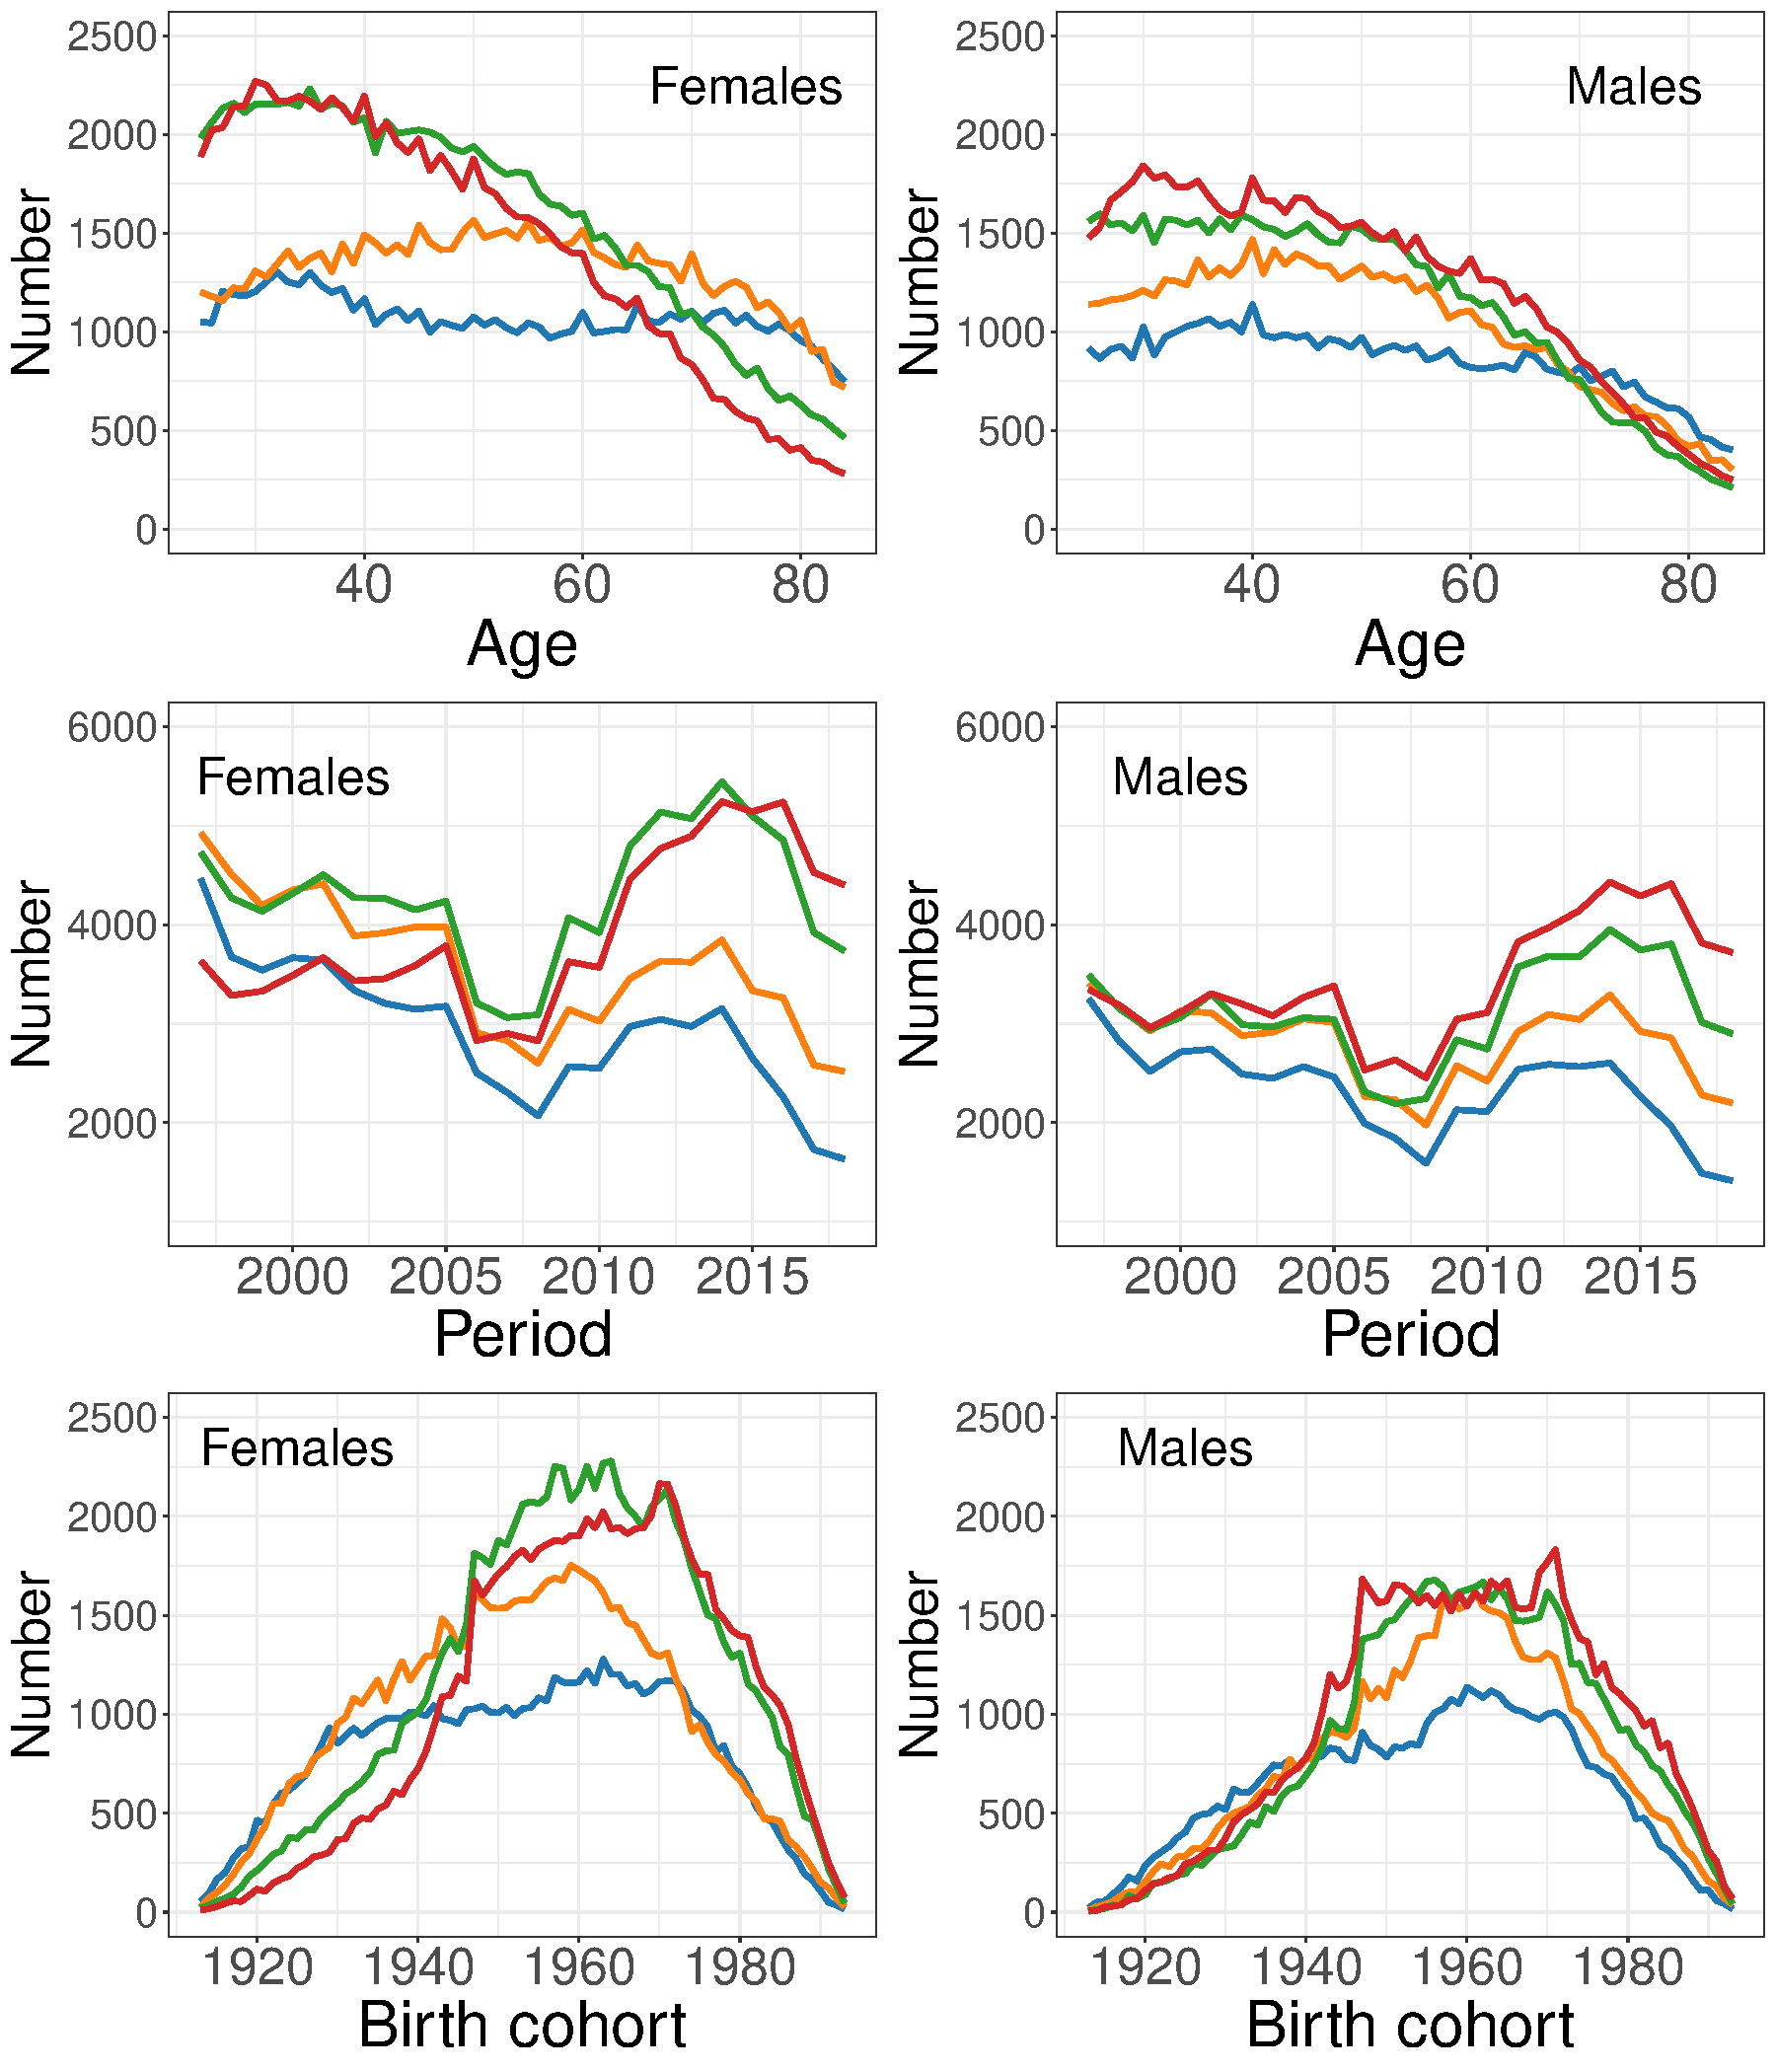
\includegraphics[width=\textwidth]{Figures/numbers.pdf}
    \end{subfigure}
    \vskip\baselineskip\vspace{-0.3cm}
    \end{minipage}%
    \begin{minipage}{.2\textwidth}
        \hfill\vspace{-1.0cm}
        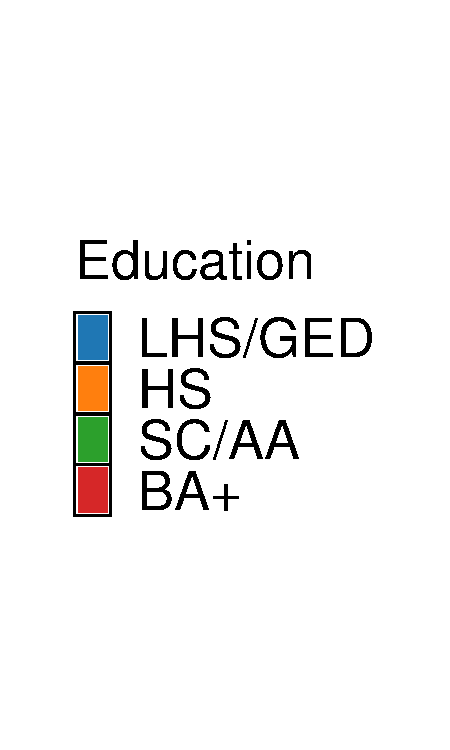
\includegraphics[width = \textwidth]{Figures/number_prop_legend_m.pdf}
    \end{minipage}
    \caption{The number of (left) female and (right) male participants in the survey data grouped by age group, period, and birth cohort, separated by level of attained education.}
    \label{figure:data_numb}
\end{figure}

\begin{figure}[!ht]
  \begin{minipage}{.8\textwidth}
  \centering
  \begin{subfigure}[b]{\textwidth}   
      \centering 
      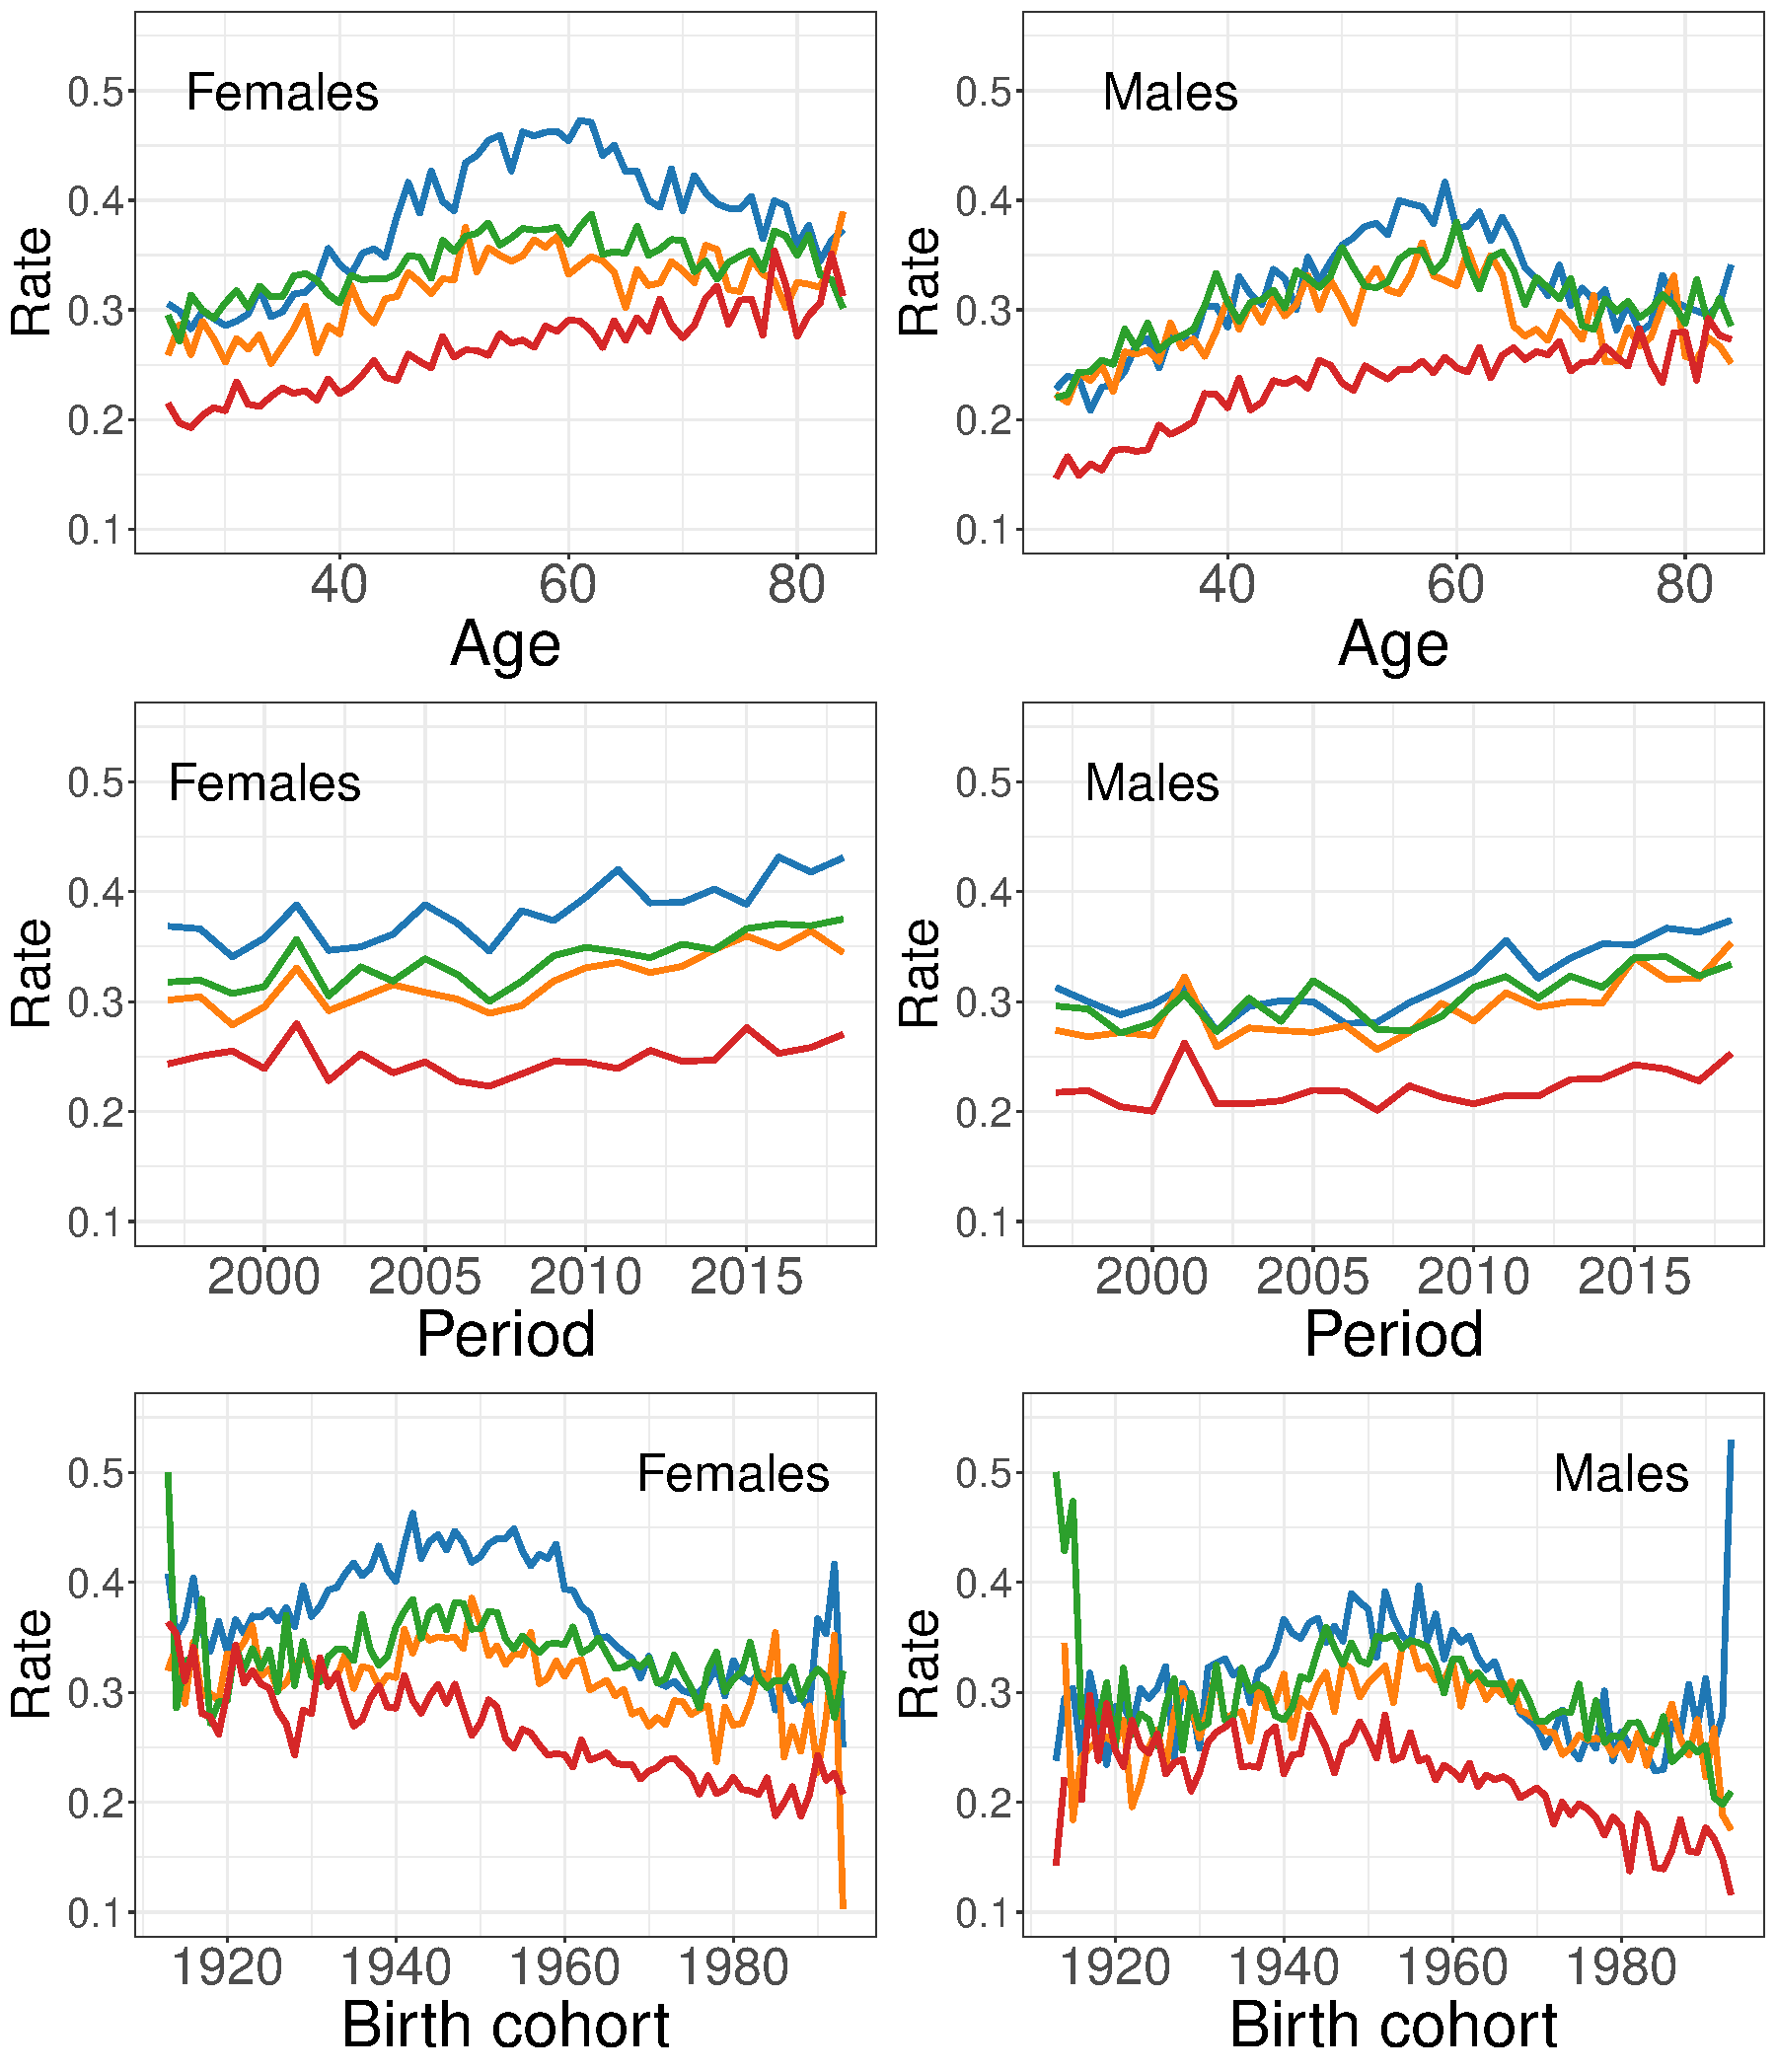
\includegraphics[width=\textwidth]{Figures/proportions.pdf}
  \end{subfigure}
  \vskip\baselineskip\vspace{-0.3cm}
  \end{minipage}%
  \begin{minipage}{.2\textwidth}
      \hfill\vspace{-1.0cm}
      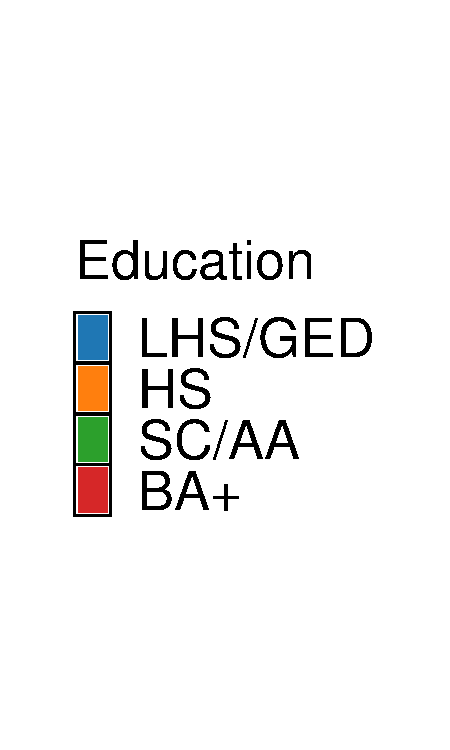
\includegraphics[width = \textwidth]{Figures/number_prop_legend_m.pdf}
  \end{minipage}
  \caption{The proportion of (left) female and (right) male participants with back pain in the survey data grouped by age group, period, and birth cohort, separated by level of attained education.}
  \label{figure:data_prop}
\end{figure}

The proportion of participants reporting back pain, stratified by level of education in each age group, period and birth cohort is shown in Figure \ref{figure:data_prop}, side by side for females and males. In both females and males, over age, the proportions appears to be generally increasing until age $60$ after which it decreases among participants with LHS/GED level of attained education, while remaining almost constant for the others. Over periods, the proportions appears to be nearly constant or slightly increasing for both females and males in all levels of attained education. Over cohorts, the proportions are either slightly increasing or constant between the $1913$ and $1950$ birth cohorts. In more recent cohorts after the $1950$ birth cohort, the proportions appear to decrease for all levels of attained education. Across all three temporal indices, it is evident that participants with BA+ level of attained education generally experienced back pain more seldom than the lower levels of attained education. Conversely, participants with the lowest level of education, LHS/GED, appears to generally have experienced the highest proportions of back pain over all three temporal indices. For the two other levels of attained education, HS and SC/AA, their proportions of individuals with back pain generally appear to be closer to that of LHS/GED than BA+. 

Figures \ref{figure:explorative:rateplot_age_f} and \ref{figure:explorative:rateplot_age_m} show the rate of back pain over the years of observation in survey participants grouped by age for females and males, respectively. Within all age groups, for all levels of attained education, the rate appears to be either slightly increasing or constant, albeit with some fluctuation. Across levels of education, we observe different rates, with the highest-observed rate for LHS/GED level ($25\%$ to $50\%$), and the lowest-observed rate for BA+ level ($19\%$ to $35\%$). For HS and SC/AA levels of attained education, the rate appears to be similar over periods. Interestingly, among participants with GED/LHS level of attained education, the rate between age groups differs the most compared to all other levels of attained education. In both figures, as we advance through the age groups from youngest to oldest, we observe, for all levels of attained education, increasing rate until age the groups $55$ to $64$, after which the rate begins to decrease. 

\begin{figure}[!ht]
    \centering
    \begin{minipage}{.5\textwidth}
      \centering
      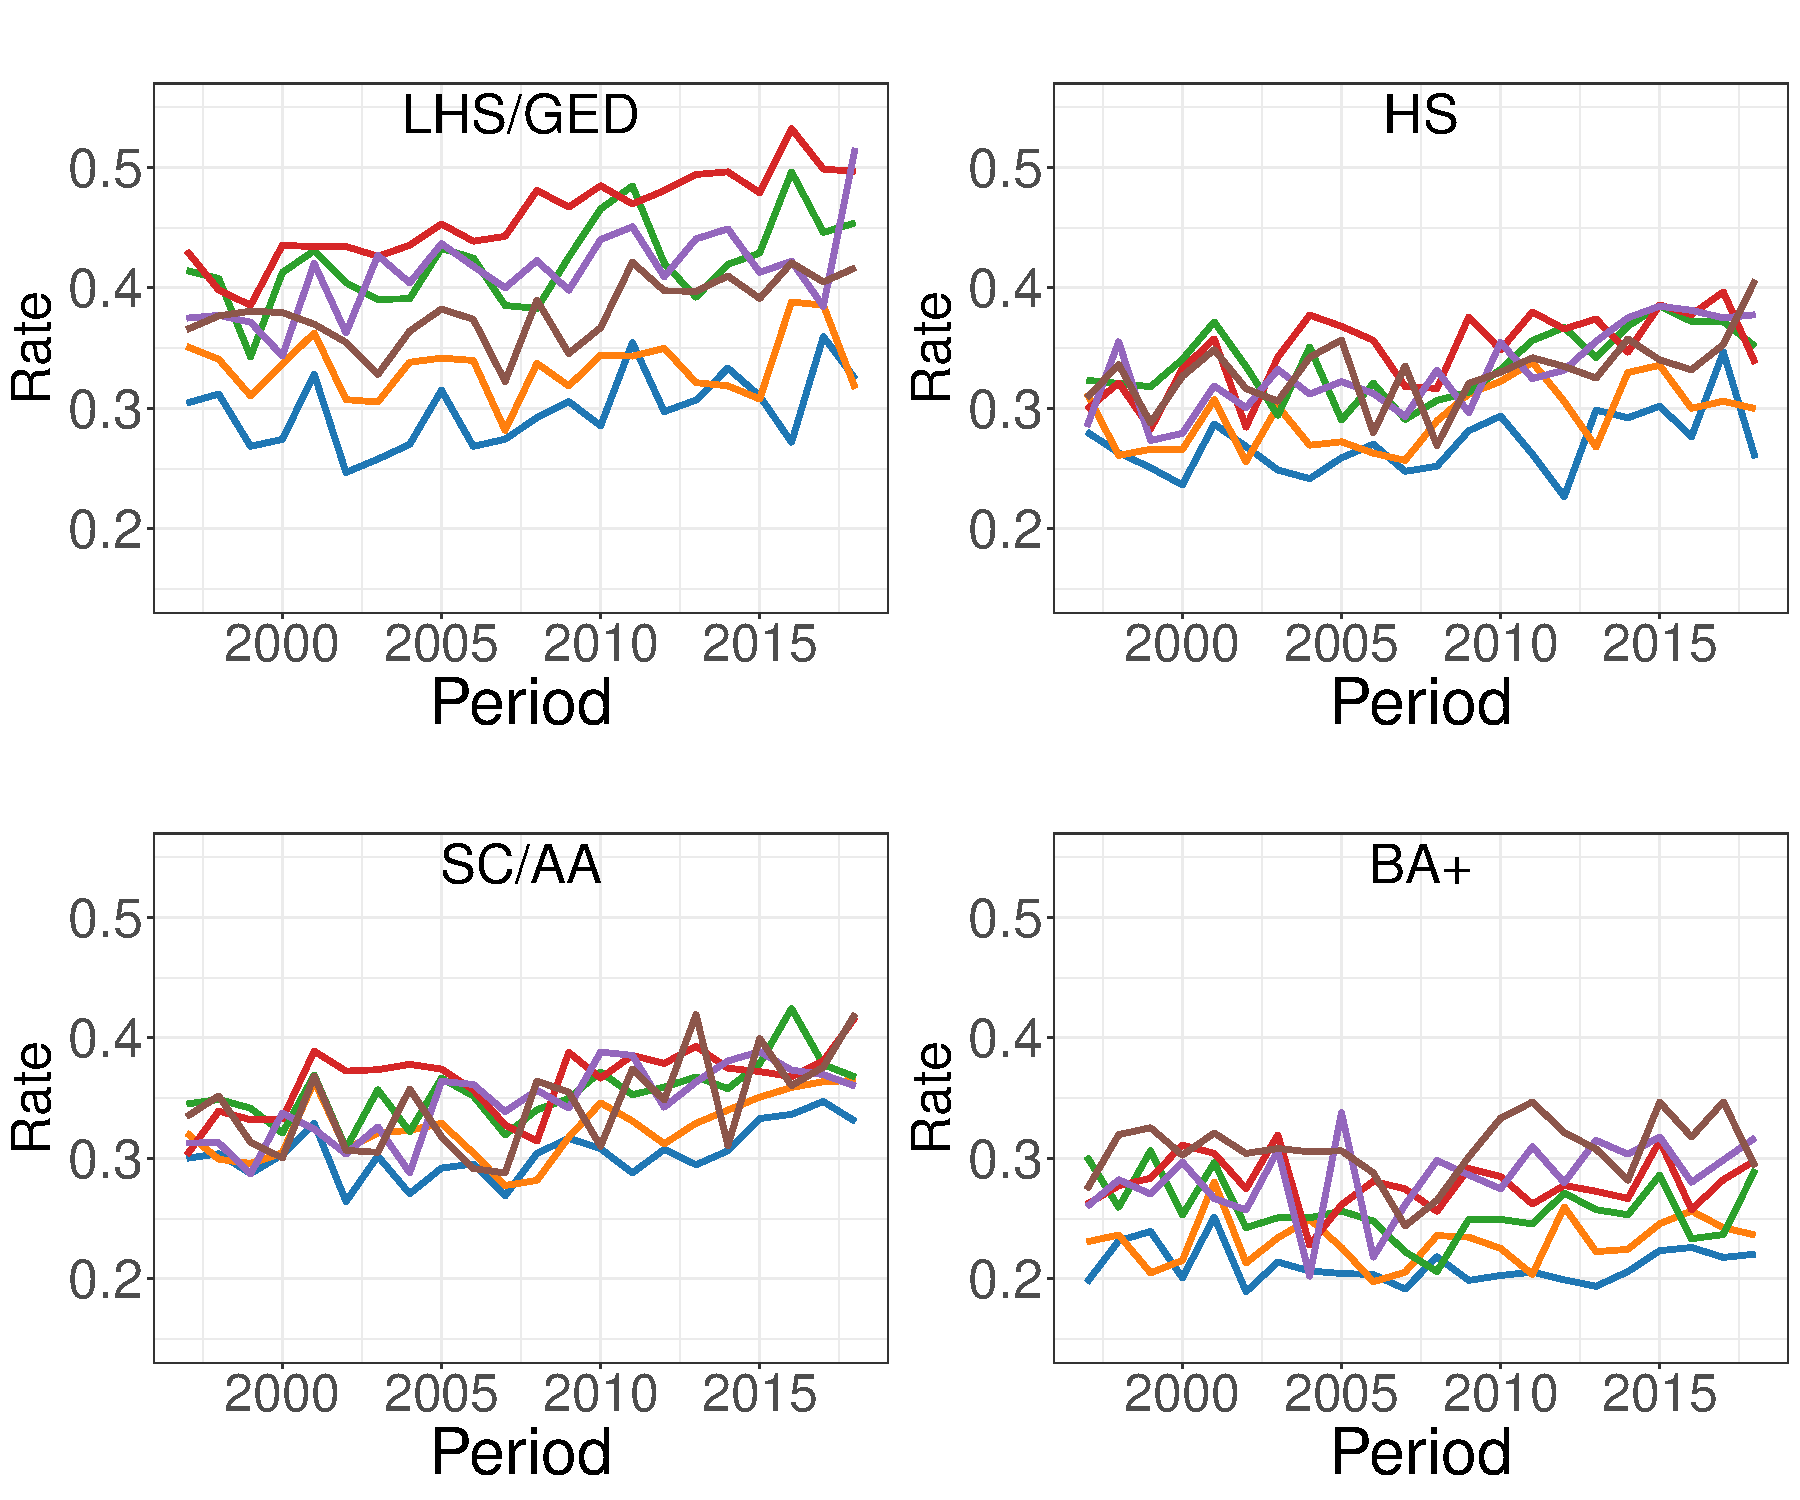
\includegraphics[width=1.6\linewidth]{Figures/rateplot_age_f.pdf}
    \end{minipage}%
    \begin{minipage}{.5\textwidth}
      \hfill
      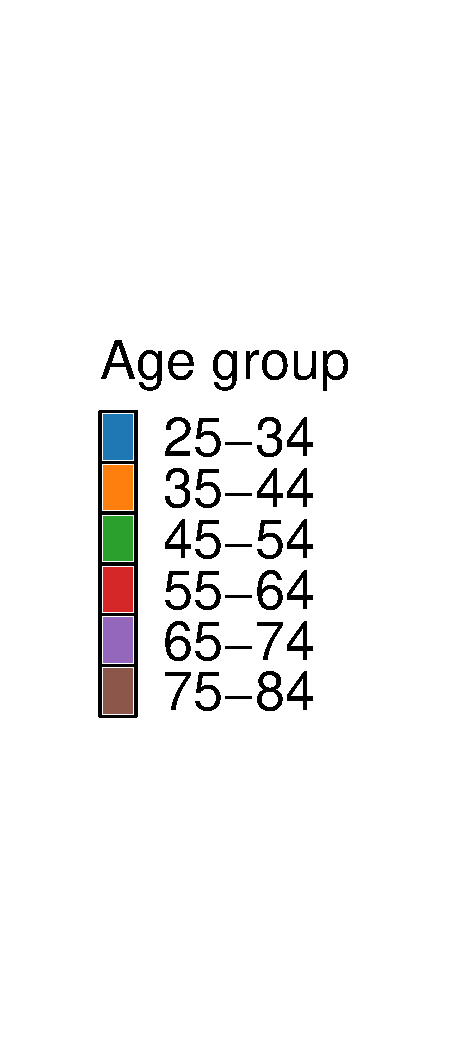
\includegraphics[width=0.4\linewidth]{Figures/rateplot_age_legend_f.pdf}
    \end{minipage}
    \caption{The proportion of female survey participants with back pain over periods, grouped into $6$ groups by age for each level of attained education.}
    \label{figure:explorative:rateplot_age_f}
\end{figure}

\begin{figure}[!ht]
    \centering
    \begin{minipage}{.5\textwidth}
      \centering
      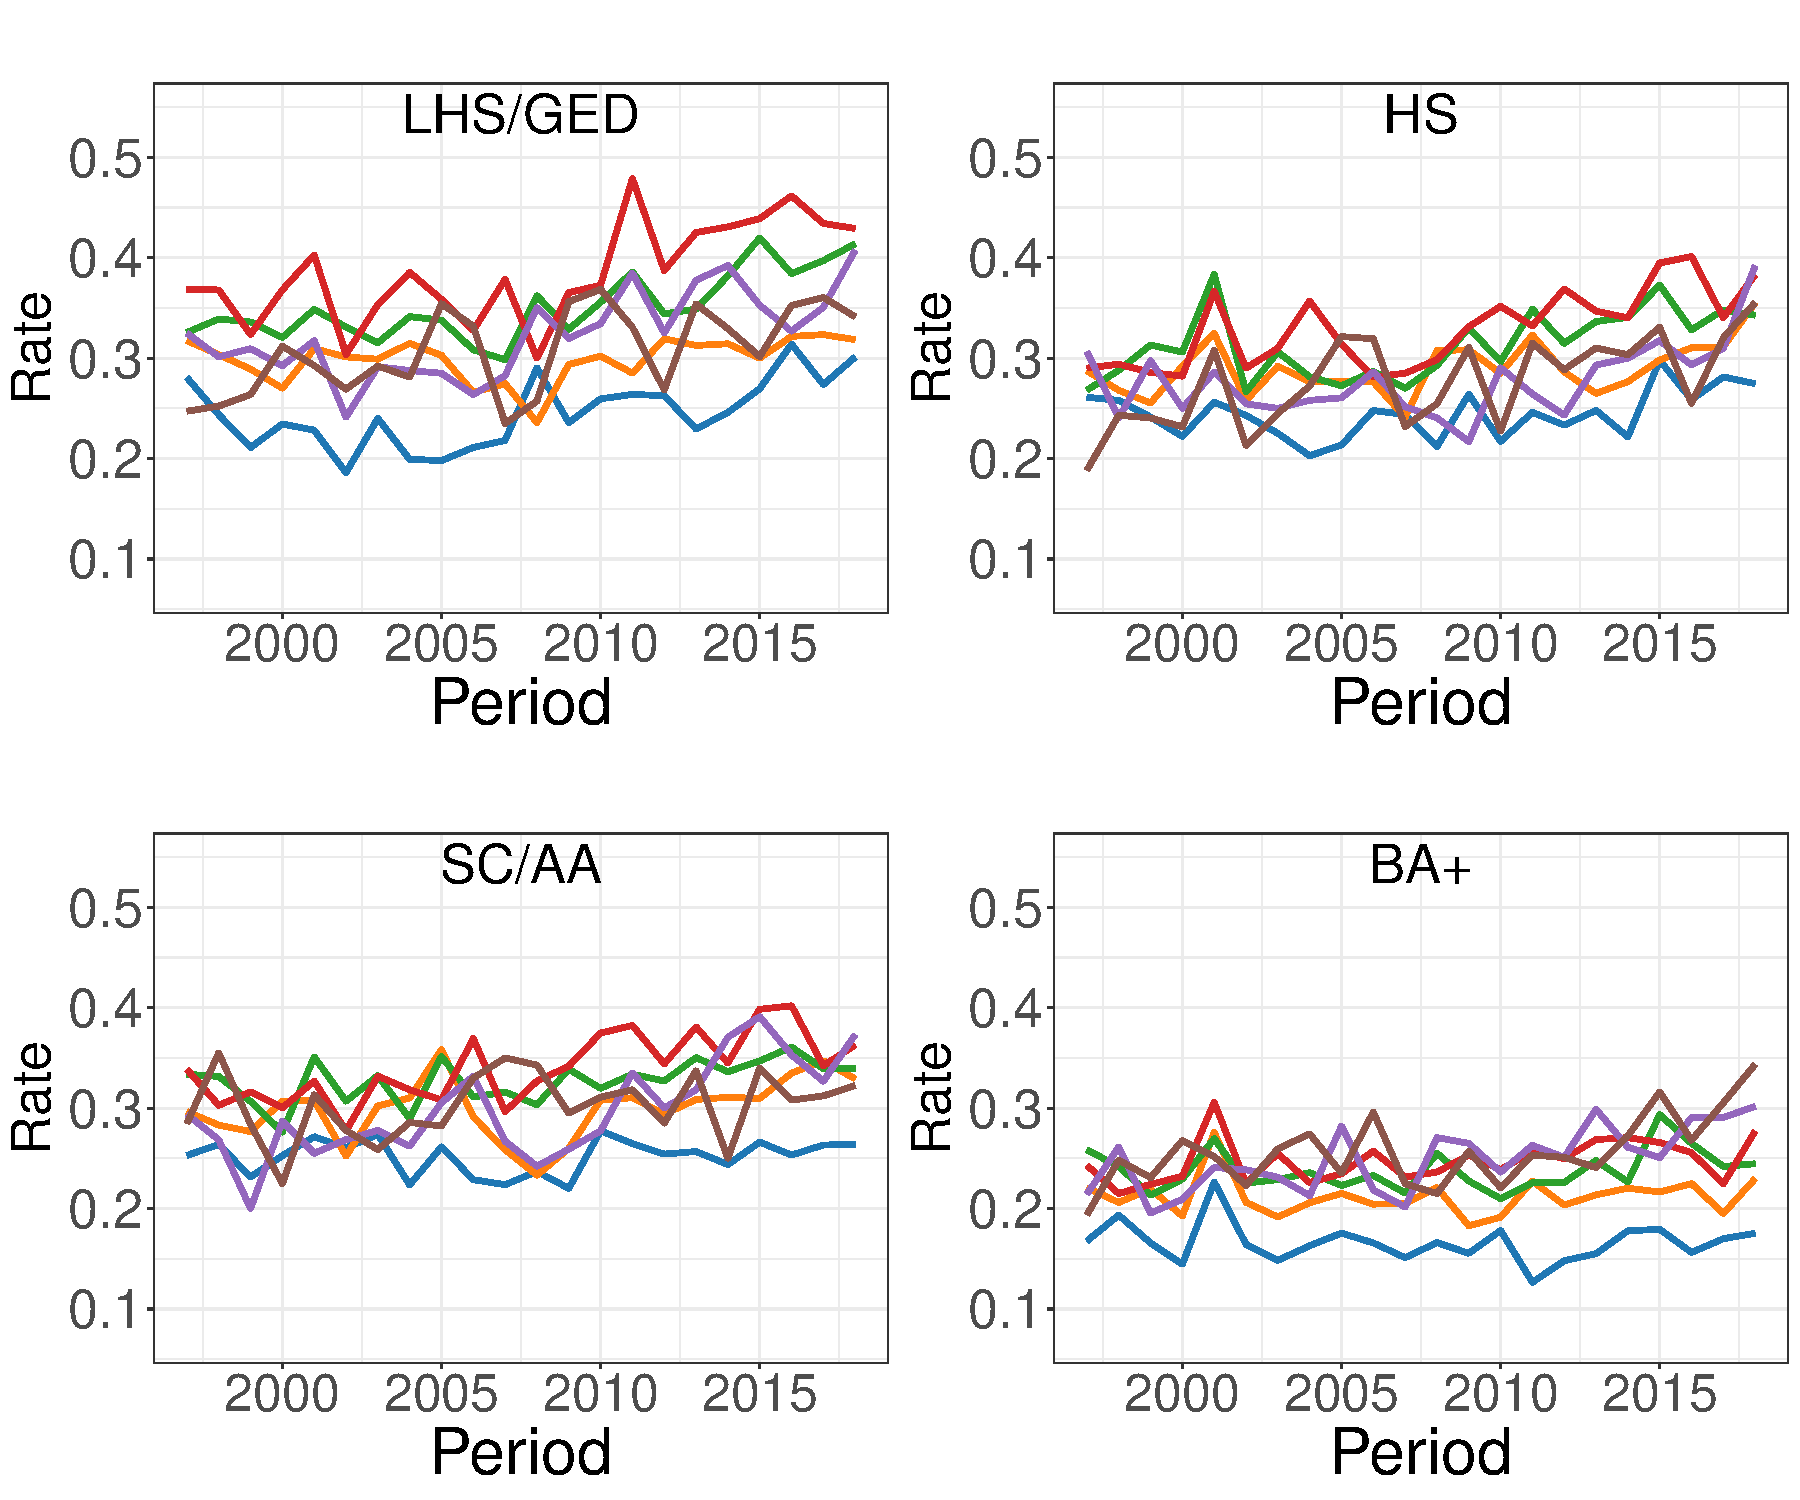
\includegraphics[width=1.6\linewidth]{Figures/rateplot_age_m.pdf}
    \end{minipage}%
    \begin{minipage}{.5\textwidth}
      \hfill
      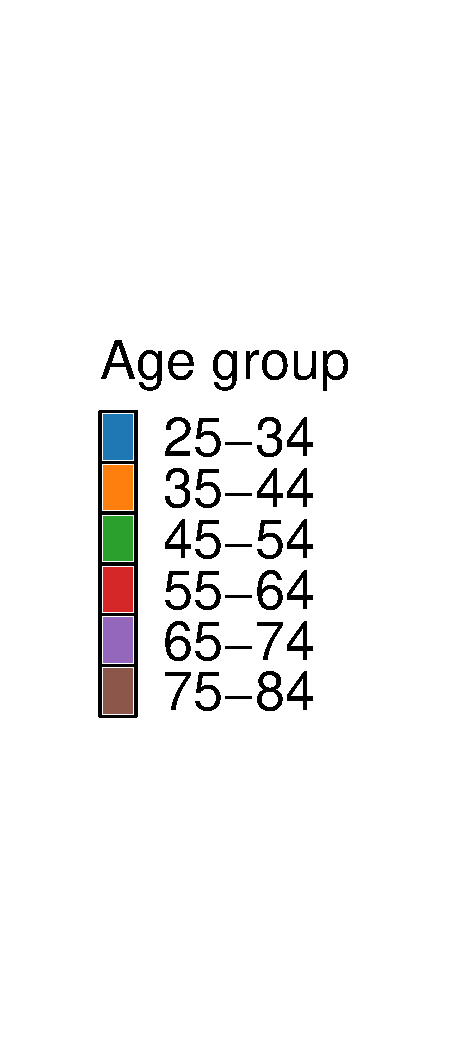
\includegraphics[width=0.4\linewidth]{Figures/rateplot_age_legend_m.pdf}
    \end{minipage}
    \caption{The proportion of male survey participants with back pain over periods, grouped into $6$ groups by age for each level of attained education.}
    \label{figure:explorative:rateplot_age_m}
\end{figure}

Figures \ref{figure:explorative:rateplot_cohort_f} and \ref{figure:explorative:rateplot_cohort_m} show the rate of back pain over the years of observation in survey participants grouped by generation (over several birth cohorts) for females and males, respectively. Generally, within all educational groups, we observe a larger rate of back pain in older generations and smaller rates for more recent generations. For the newest generation, the rate is particularly low among participants with the lowest level of attained education. For the oldest generation, however, more variability is observed, making it difficult to compare with the others. This variability is somewhat expected, as the sample size from the oldest generation is quite small, and the low rate of back pain could be due to the exceptionally good health of the survivors of this generation. This is reminiscent of an effect well known in demography, known as selective mortality \citep{beckett2000converging, house1990age, lynch2003cohort}. As with the effects grouped by age, the rate of back pain in all levels of education appears to be either constant or somewhat increasing. 


\begin{figure}[!ht]
    \centering
    \begin{minipage}{.5\textwidth}
      \centering
      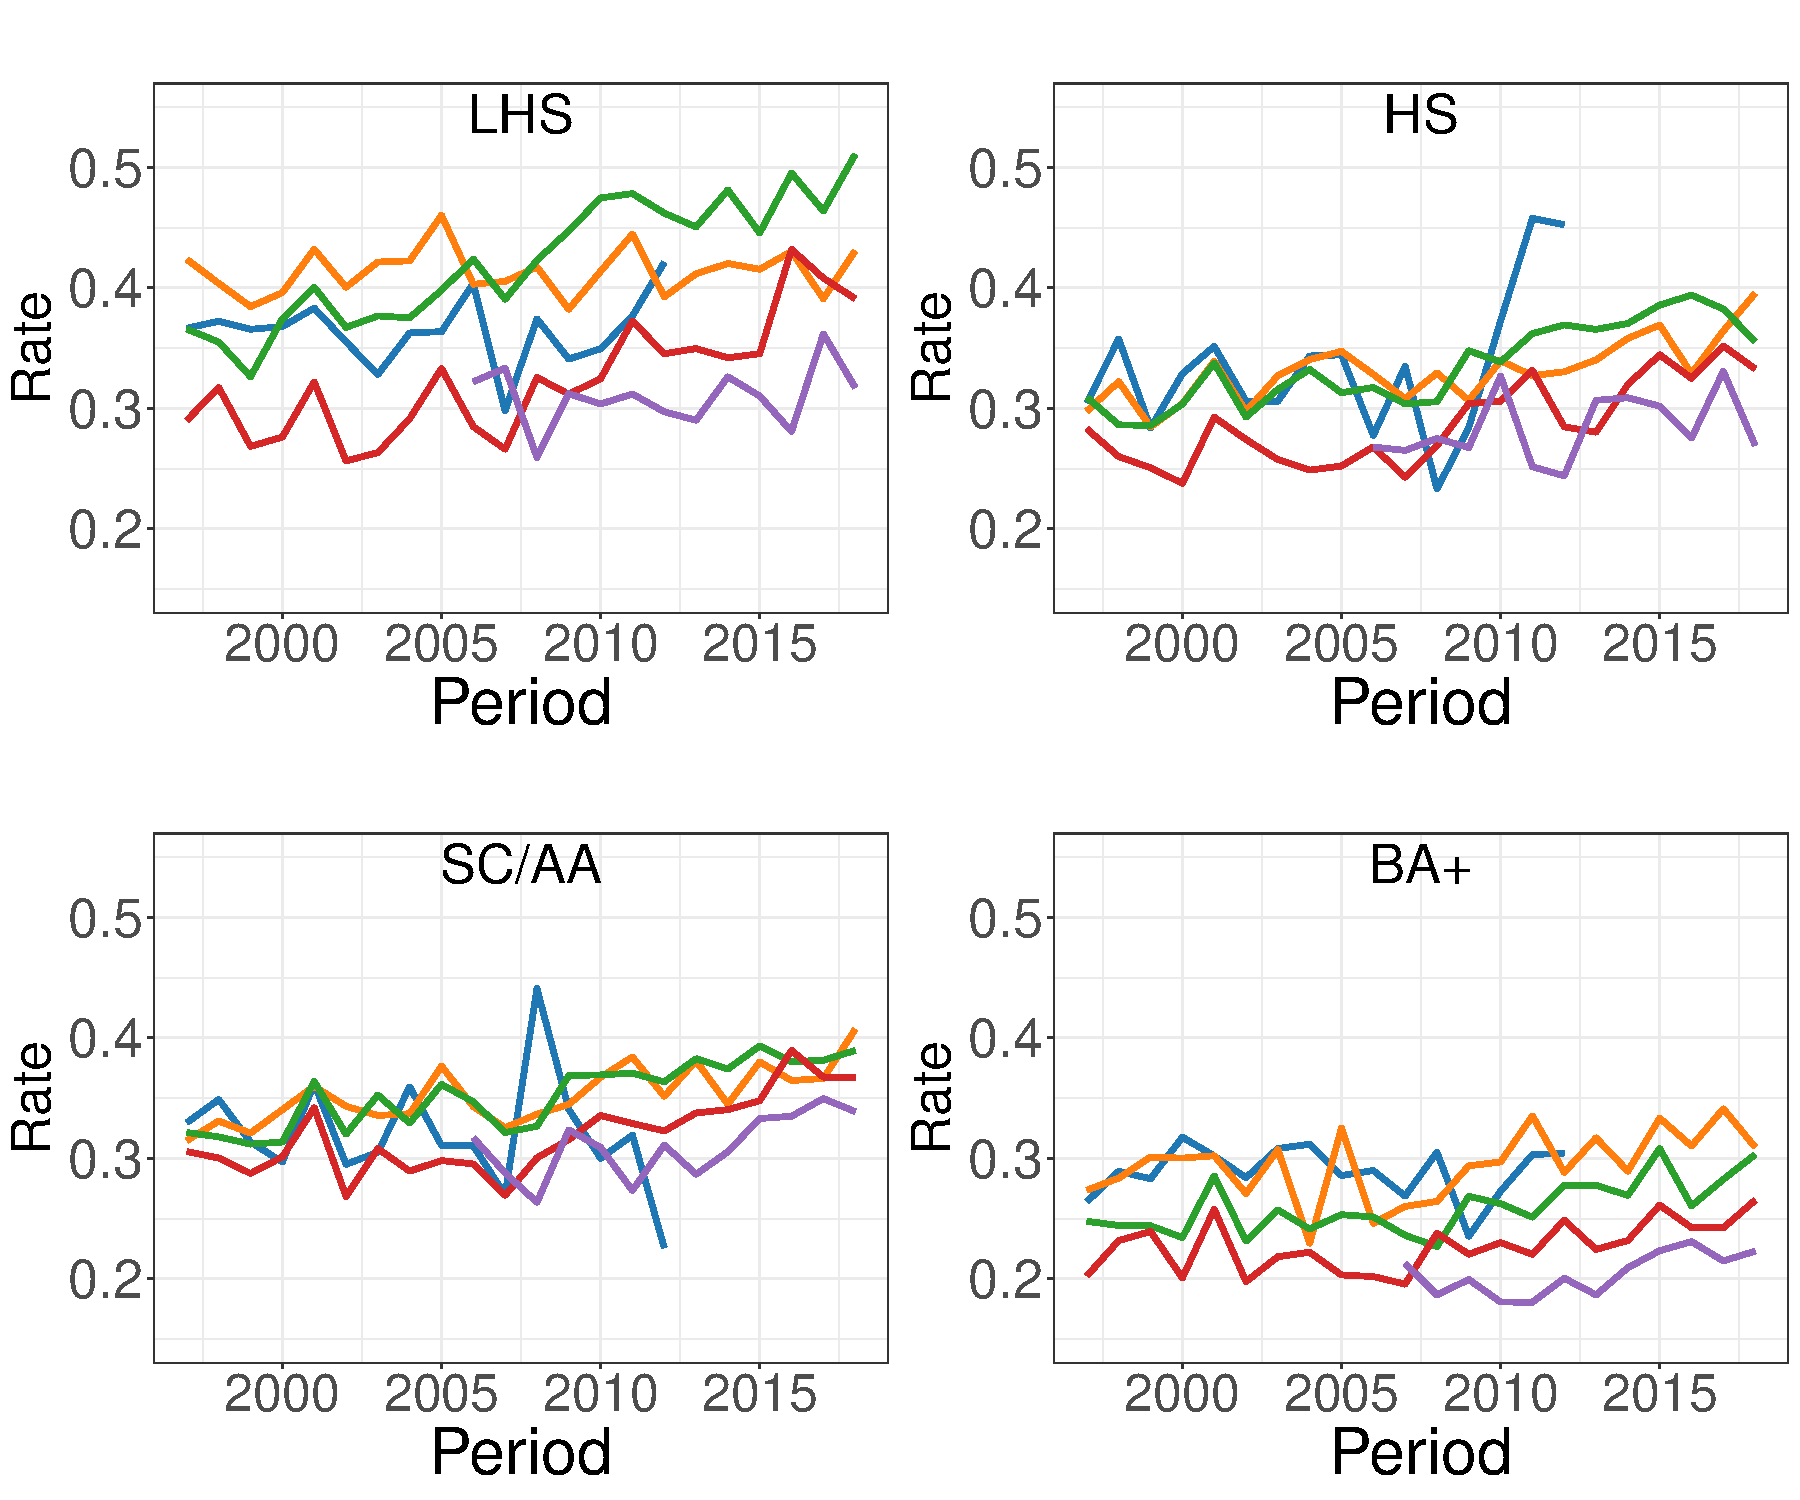
\includegraphics[width=1.6\linewidth]{Figures/rateplot_cohort_f.pdf}
    \end{minipage}%
    \begin{minipage}{.5\textwidth}
      \hfill
      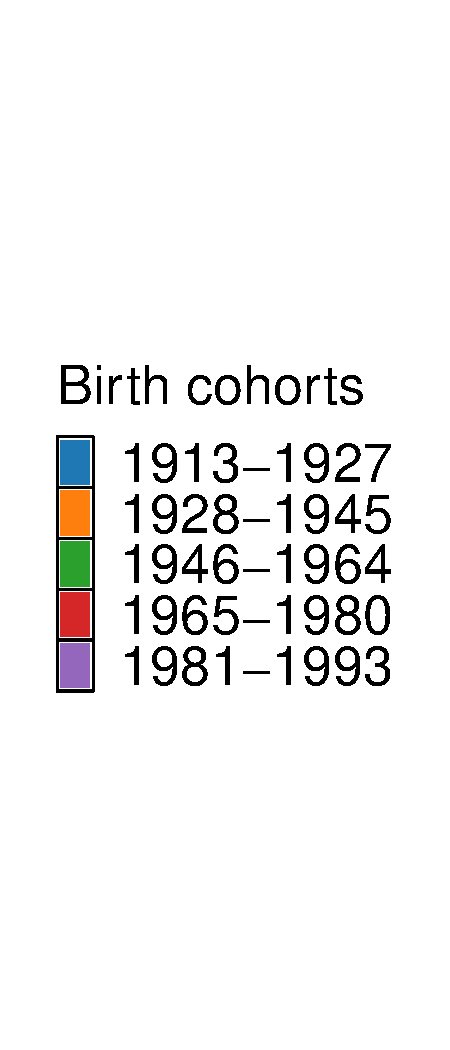
\includegraphics[width=0.4\linewidth]{Figures/rateplot_cohort_legend_f.pdf}
    \end{minipage}
    \caption{The proportion of female survey participants with back pain over cohorts, grouped into $6$ groups by age for each level of attained education.}
    \label{figure:explorative:rateplot_cohort_f}
\end{figure}

\begin{figure}[!ht]
    \centering
    \begin{minipage}{.5\textwidth}
      \centering
      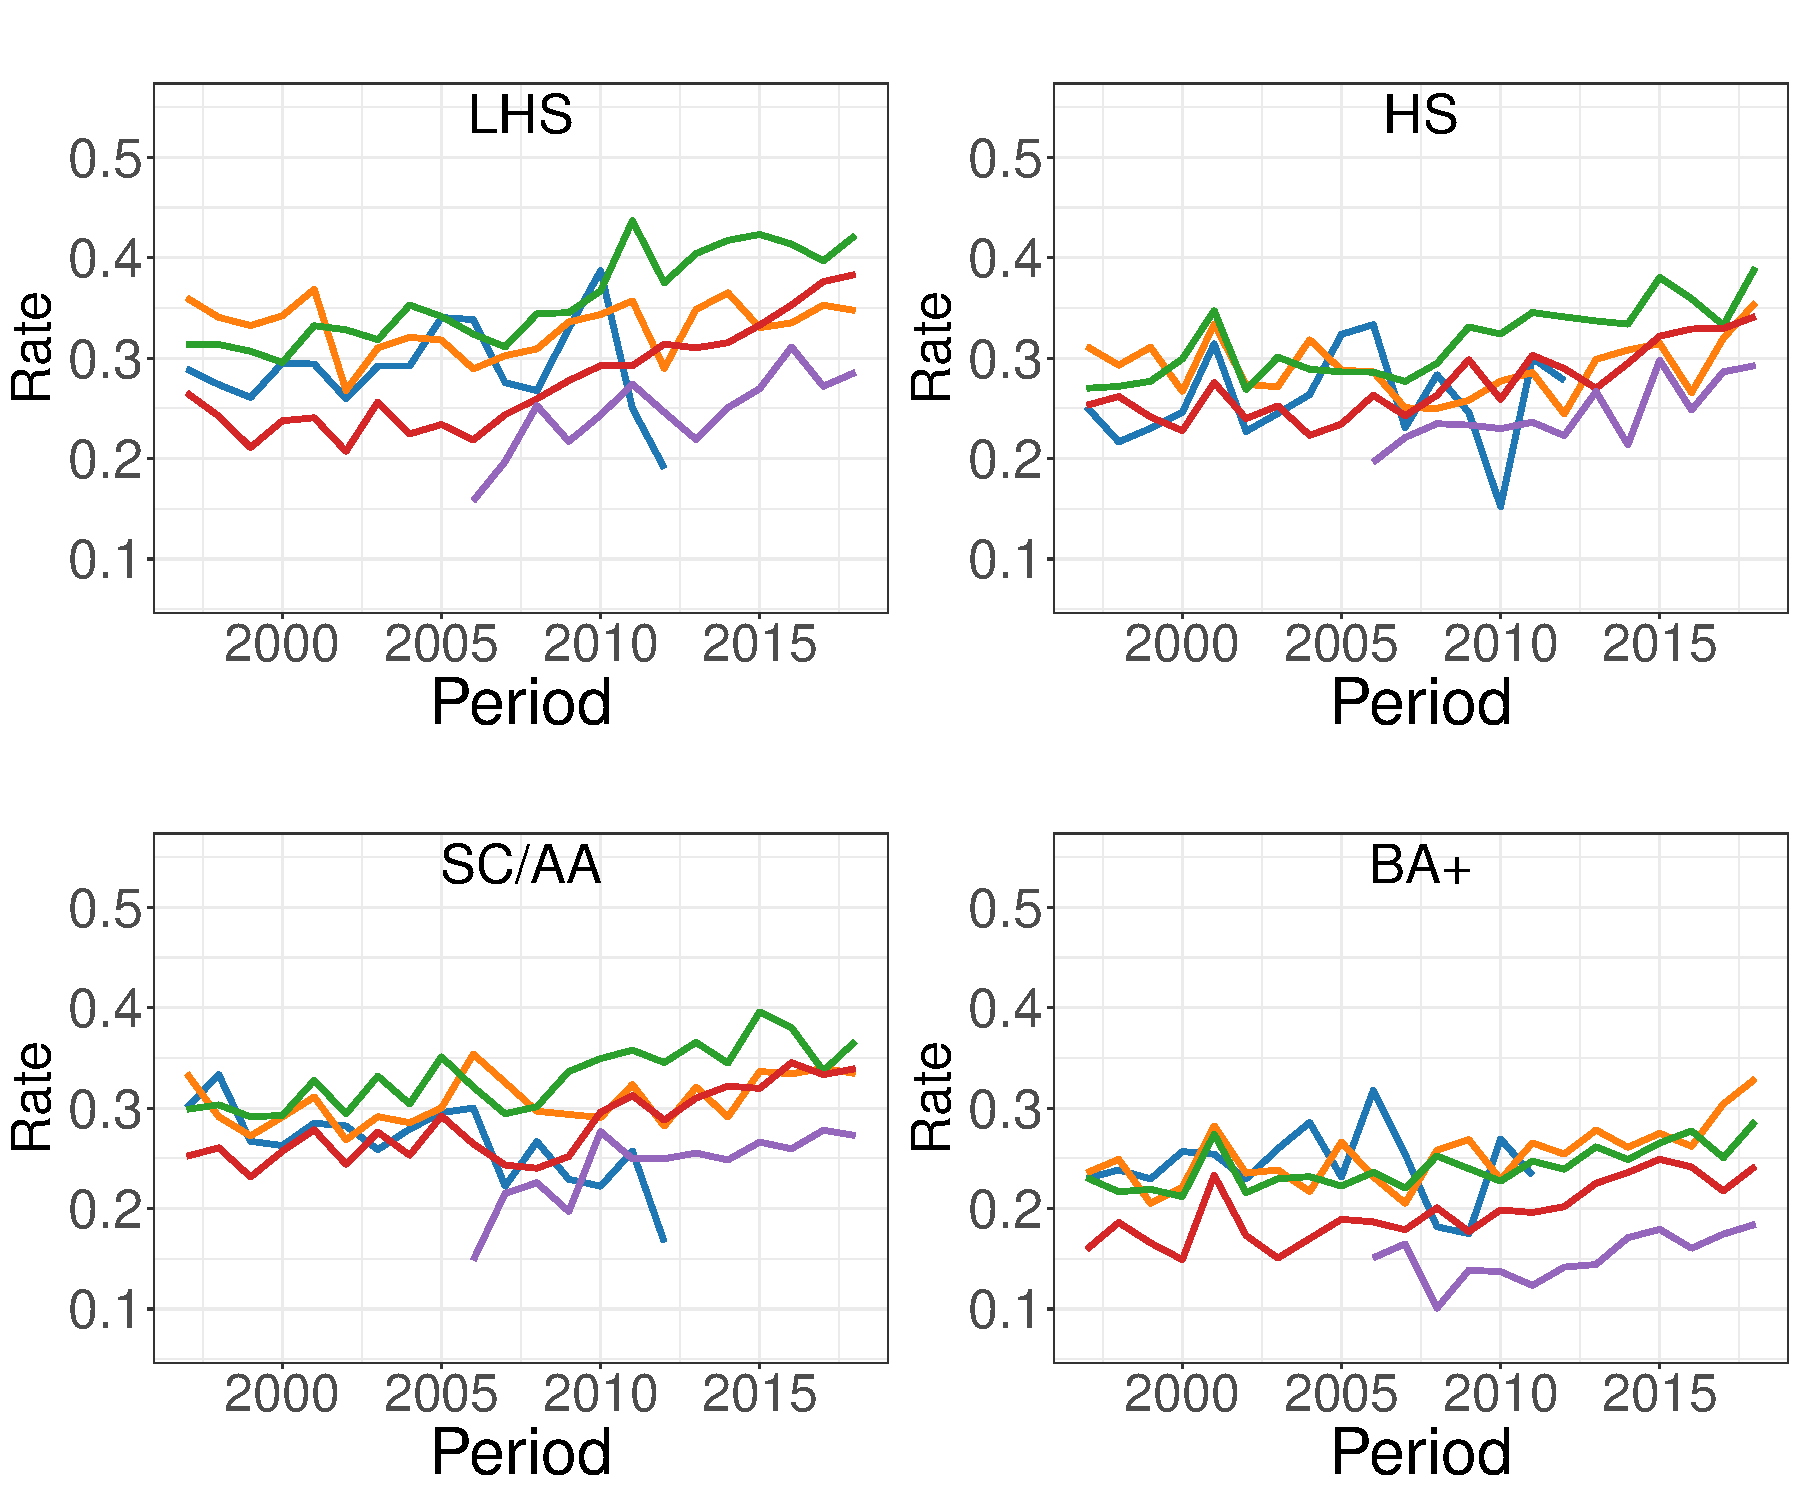
\includegraphics[width=1.6\linewidth]{Figures/rateplot_cohort_m.pdf}
    \end{minipage}%
    \begin{minipage}{.5\textwidth}
      \hfill
      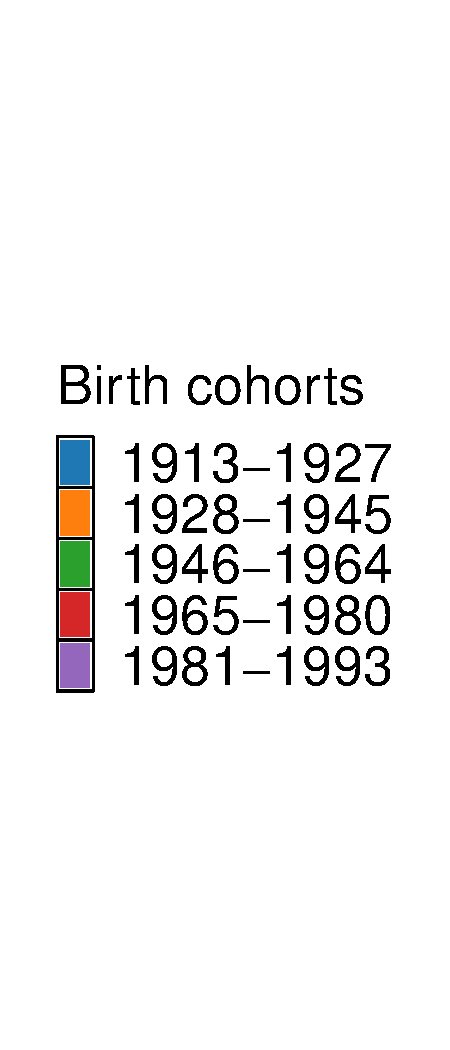
\includegraphics[width=0.4\linewidth]{Figures/rateplot_cohort_legend_m.pdf}
    \end{minipage}
    \caption{The proportion of male survey participants with back pain over cohorts, grouped into $6$ groups by age for each level of attained education.}
    \label{figure:explorative:rateplot_cohort_m}
\end{figure}

By this simple exploratory analysis, we may theorize on what to expect from the analysis by MAPC models. Firstly, as the rate of back pain stratified by attained education remains almost constant over periods in several age groups and cohorts, we do not expect the period as a temporal scale to be of large significance in explaining the observed temporal variability. Moreover, due to the observable differences in rate based on age groups for all levels of education, it is expected that age as a temporal scale will be of great significance. Since these differences in rate based on age groups were particularly pronounced for LHS/GED level of attained education, we expect this to be reflected in our models. The same is said for cohort, as similar observations were made over this temporal scale and the differences are more pronounced for the LHS/GED level. In addition, since it is clear that participants with BA+ level of attained education generally had better health outcomes and had larger sample sizes over all temporal indices, it would be sensible to pick this level of attained education as our baseline level of attained education for later inference across levels of attained education.












\FloatBarrier
\newpage
\clearpage

\section{Age-Period-Cohort models}\label{section:Age-period-cohort-models}
Age-period-cohort (APC) models analyse incidence, morbidity, or prevalence rates of diseases or conditions of interest in a temporal fashion by stratifying the observations by age group and observation period \citep{APC-OLD, APC-OLD-2, APC-OLD-3}. Age simply refers to the age of the observed participants at a certain point in time (i.e., period). Consequently, knowing the age of observed participants along with the period of observation, we obtain a perfect linear relationship to determine the birth cohorts of the observed participants, giving us the final cohort term of the model. A major consideration with the APC model lies in selecting the method to remedy the infamous problem of identifiability of the temporal effects \citep{APC-wakefield}. The family of APC models have become prominent in temporal analyses in recent decades, and variants have been proposed to remedy this problem in both frequentist \citep{Rosenberg2023} and Bayesian frameworks \citep{berzuini1993bayesian,berzuini1994bayesian}, each carrying their own advantages and disadvantages. For the application of the APC model in this thesis, we stick to the Bayesian framework of APC models \citep{APC-Bayesian-Yang,APC-Bayesian-Held}, the implications of which are elaborated upon in Section \ref{section:BayesianInference}. The multivariate extension of the APC model, the multivariate APC (MAPC) model \citep{hansell2003copd, jacobsen2004women}, facilitates stratification by factors such as geographic region, income, and in our case, level of attained education. Incorporating several strata into the model entails some additional considerations in the inference of the model, but also provides remedies to the identifiability problem \citep{APC-Bayesian-Andrea}.

In this section, we first provide basic intuition on temporal analyses and what they measure in Section \ref{section:lexis}, before introducing the APC model in its simplest univariate form in Section \ref{section:univariateAPC}. The extension from the univariate APC model to the multivariate APC model then follows in Section \ref{section:multivariate} and the methods of cross-strata inference in the multivariate APC in Section \ref{section:APC-inference}.

\subsection{The Lexis diagram}
\label{section:lexis}
In the application of APC models, the observed data, typically mortality, prevalence, or incidence rates, are represented by the Lexis diagram \citep{Lexis,Lexis2}. The Lexis diagram is a two-dimensional tabulated format for graphical representation of the data, in which the temporal indices "age" and "period" make up the vertical and horizontal axes, respectively. The axes are divided into discrete intervals, typically by calendar years, meaning each interval on the age axis makes up a compartment with each interval on the period axis. Each compartment refers to a group of participants with a certain age at a certain point in time (period). The compartments are filled with information pertaining to the mortality, prevalence, or incidence of a disease or condition, consequently stratifying the data by age and period. As the birth cohort is identifiable by the age and period, it is consequently represented along the diagonal of the tabular format. An example using toy-data to illustrate the Lexis diagram is shown in Figure \ref{figure:Lexis}. The data shown here could represent the number or rate of participants with a disease or condition, such as back pain.

\begin{figure}[!ht]
    \centering
    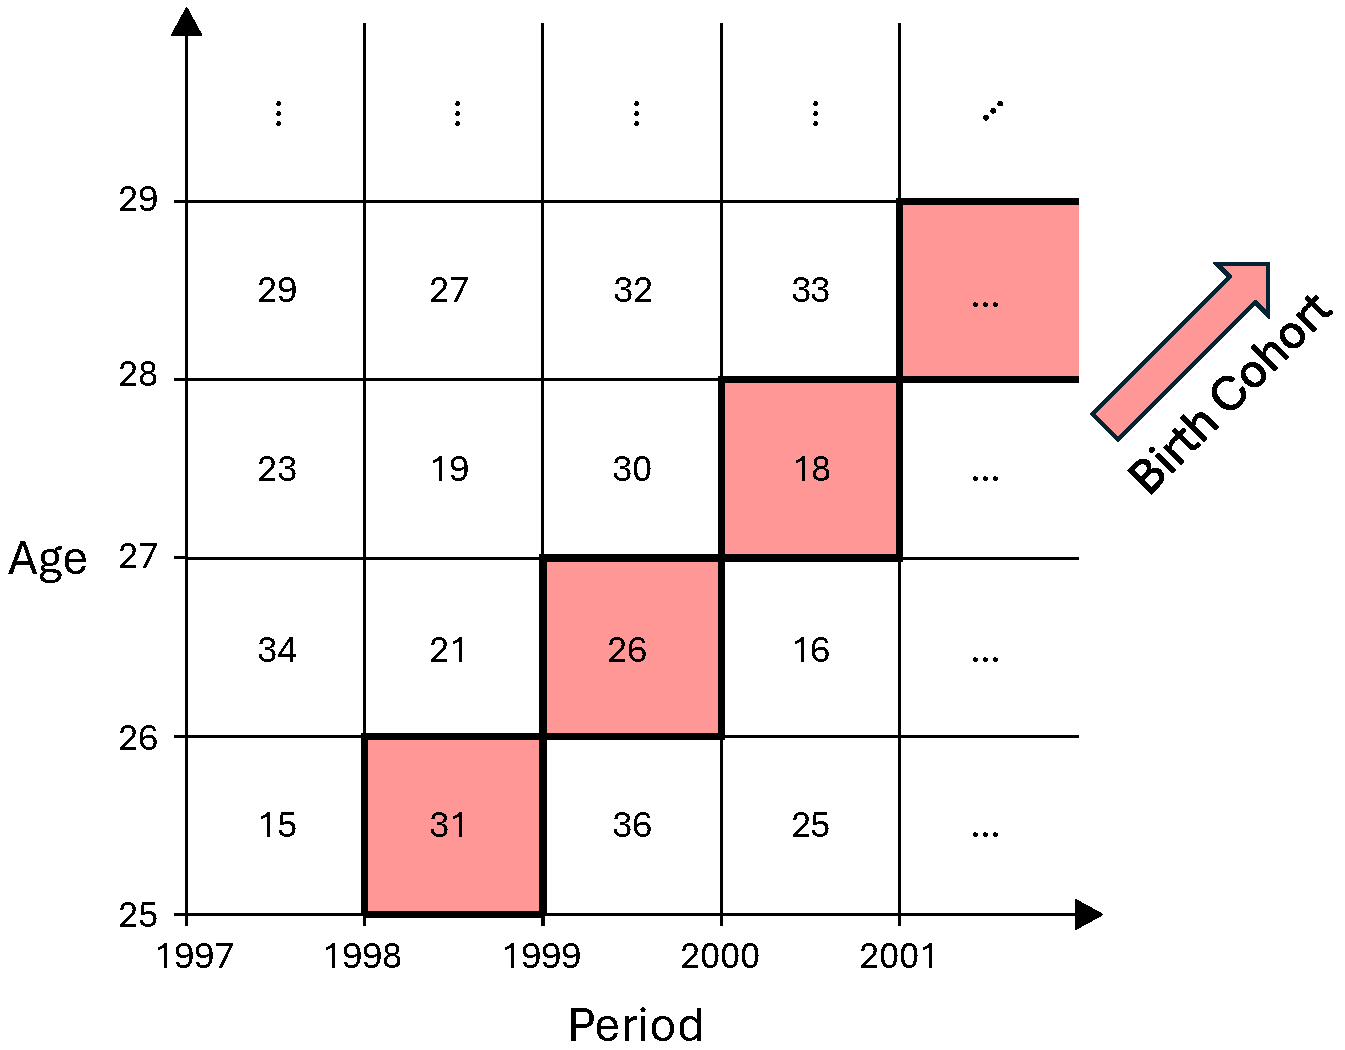
\includegraphics[width = 0.8\textwidth]{./Figures/Lexis.pdf}
    \vspace{-0.2cm}
    \caption{Lexis diagram for example data, such as prevalence of a disease or condition (back pain, in our study). On the axes are age groups and periods with an equal interval length of one year. The cohorts are represented along the diagonals, illustrating the linear dependence between the temporal indices. Marked in red is the example 1998 birth cohort.}
    \label{figure:Lexis}
\end{figure}

%Interpretation of the temporal scales
The temporal inference of the APC model is based on observations of incidences on the three different temporal scales of age, period, and cohort, and stems from proposed methods to analyse data in the format of the Lexis diagram. Though the analysis is performed with respect to time on different scales, it is important to recognize that time itself is not the cause of disease, but rather it represents a way to measure exposure of other factors that operate with time \citep{berzuini1994bayesian}. The ways that these external factors operate and affect the population may be different and difficult to measure, and each of the temporal scales captures different aspects and effects of these factors. Age as a temporal scale is a good substitution for cumulative exposure. As a person grows older, the continued exposure to factors that may cause a disease accumulates, heightening the risk of contracting the disease or condition. Meanwhile, for measuring factors applying to everyone at a certain point in time, the period as a temporal scale is useful. This temporal scale captures shocks, such as sudden outbreaks or major scale events (war, natural disaster, etc.), carrying consequences for the disease or condition of interest. Finally, examining the data using cohorts as a temporal scale helps identify the impact of factors that has changed gradually over time and generations, such as the evolving health habits in the general population or living conditions.

\subsection{The univariate age-period-cohort model}\label{section:univariateAPC}
First, let us define the univariate APC model mathematically. Let $n_{ij}$ denote the number of participants at risk in age group $i$ $(i = 1,...,I)$, with observations taken in period $j$ $(j = 1,...,J)$, stemming from the birth cohort $k$ $(k=1,..,K)$. As the index $k$ may always be derived from $i$ and $j$, it is consequently omitted from notation when accompanied by $i$ and $j$. Furthermore, we assume that the discrete number of observed incidents $y_{ij}$ follows a binomial distribution with the probability of back pain $\pi_{ij}$ and number of trials $n_{ij}$, corresponding to the size of the respective group. Since our application examines a dichotomous outcome noting observations of both presence and absence of back pain, a binomial model is suitable. With the assumption of independent observations, the joint likelihood may be written as a product of binomial terms. In applications, several discrete probability distributions such as the Poisson (as in the original formulation by \cite{clayton1987models}) and negative binomial distributions may be used, though we only consider the case of binomial likelihood (for the application at hand). With these assumptions, the univariate APC model models the log-odds probability of back pain $\pi_{ij}$ as a linear predictor with an overall intercept $\mu$, age effects $\theta_i$, period effects $\phi_j$, and cohort effects $\psi_k$. That is,
\begin{equation}
    \log\left(\frac{\pi_{ij}}{1-\pi_{ij}}\right) = \mu + \theta_i + \phi_j +\psi_k.
\end{equation} 
To ensure identifiability of the intercept, sum-to-zero constraints are typically imposed on $\pmb \theta$, $\pmb \phi$ and $\pmb \psi$. An interesting area of discussion for this model revolves around the perfect linear combinations between the three temporal indices, since the cohort index is directly derived from the age and period index as $k = I-i+j$. Due to the linear dependence of the cohort index on the age and period indices, a second constraint is required to identify the separate contributions of the three temporal effects. For equally-spaced data, this is evident as changes in linear trends only cause a change in the estimated set of parameters all while keeping the linear predictor the same \citep{riebler2010multivariate}. As a consequence, only non-linear trends, such as second differences, are identifiable \citep{clayton1987models}. Particular considerations occur when age and period are defined on different time grids, with different granularity (i.e. month and year). Since we will be using the same granularity for all our temporal indices, these considerations are not covered here, though  further details are provided by \cite{riebler2010multivariate}.

%Resolutions to the identifiability problem
In frequentist settings, the additional constraint has been imposed in several ways with many proposed remedies. These remedies include fixing one temporal effect to zero, equating two effects at one time point \citep{fienberg1979identification}, including additional covariates, or introducing penalty functions to be minimized \citep{osmond1982age}. While these remedies ensure identifiable effects, they are also only identifiable in the context of the imposed constraint, and are therefore difficult to interpret without expert knowledge. In our case, we stick to the Bayesian framework to provide model fit, and make use of the upcoming multivariate version of the APC model to remedy the problem. 

\subsection{The multivariate age-period-cohort (MAPC) model}
\label{section:multivariate}
In several applications, such as ours, it is desirable to compare temporal trends for different strata defined in terms of education, health outcome, sex, activity, or some other factor. While it is possible to use separate APC models for each stratum, especially when prediction is of interest, the issue of identifiability makes comparison between the strata difficult and unintuitive. For these contexts, it is better to use a multivariate APC model to investigate heterogeneous temporal trends. This requires data sets over the same periods and age groups for each stratum that we wish to include in the model. In terms of the Lexis diagrams introduced in Section \ref{section:lexis}, this equates to having multiple diagrams, one for each stratum. For example, one may consider that each compartment of the diagram has observations for each stratum. The multivariate APC models captures the heterogeneous time trends across the different strata, and for comparable strata, the similar factors are likely to work on the same time scales. In applications, it is useful to consider whether an effect should be shared across the different strata. For instance, consider a model where the age effect is shared across the different strata. Following the extension from the univariate APC model to the multivariate APC model by \cite{riebler2010multivariate}, this model would read
\begin{equation}
    y_{ijr}\mid \pi_{ijr} \sim \text{Binomial}(\pi_{ijr}, n_{ijr}),
    \label{eqn:likelihood-MAPC}
\end{equation}
where $y_{ijr}$ is the observed number of cases for age group $i$ in period $j$ from cohort $k$ (omitted as it depends on $i$ and $j$) following strata $r$ ($r=1,...,R$), and $n_{ijr}$ is the size of the group. The linear predictor for the log-odds of $\pi_{ijr}$ is then
\begin{equation}
    \log\left(\frac{\pi_{ijr}}{1-\pi_{ijr}}\right) = \mu_r + \theta_i + \phi_{jr} + \psi_{kr},
    \label{eqn:linear-predictor}
\end{equation}
where $\mu_r$ is the stratum-specific intercept for stratum $r$, $\theta_i$ is the 
age effect shared across each stratum, and $\phi_{ir}$ is the stratum-specific period effect and $\psi_{kr}$ is the stratum-specific cohort effect. To ensure identifiability of the stratum-specific intercepts, sum-to-zero constraints are imposed on the age, period, and cohort effects. That is
\begin{equation}
    \sum_{i}\theta_i=0,\quad \sum_j\phi_{jr}=0\quad \text{and}\quad \sum_k\psi_{kr}=0\;\; \text{for all } r = 1,...,R.
\end{equation}
Adapting this model structure for different shared effects is simple, though some care has to be taken when selecting a model for a specific analysis. If the age effect across strata is of inferential importance, then the model should naturally include a stratum-specific effect over age. Similarly, if period or cohorts are of specific interest, then a different combination of shared and stratum-specific effects should be considered. Should no combination be preferred a priori, then model selection may be used to settle on a model. Note also that the multivariate formulation of the APC model adapts the same issues regarding identifiability as the univariate. The remedy used in our application is presented in Section \ref{section:APC-inference}.

For future reference of different specifications of shared and stratum-specific effects in the multivariate APC model, the abbreviation APC will be capitalized based on which effects are shared and which are stratum-specific. Effects shared across strata are shown by uppercase letters (A, P, C) and for effects that are stratum-specific we use lowercase letters (a, p, c). For instance, the above model with shared age effect, but stratum-specific period and cohort effects would be abbreviated as the Apc model. 

\subsection{Cross strata inference with MAPC models}
\label{section:APC-inference}
A major benefit of using the multivariate APC model instead of several univariate models is that differences in effects across strata become identifiable \citep{APC-Bayesian-Andrea}. While the MAPC model inherits the same issues of identifiability as the univariate APC model, the linear predictor remains identifiable, allowing differences in the linear predictor across strata to be identifiable. To elaborate, the issue in APC models of all kinds is that the age, period, and cohort effects are not identifiable by themselves, but the sum of the parts is. Consequently, by examining the cross-strata differences of these sums, we arrive at methods of inference that are identifiable and intuitive. Examining the cross strata differences between each pair of strata is unadvised, since there are many pairs to consider, thus making interpretation difficult. Rather, it is common to analyse differences with respect to only one stratum, which is chosen subjectively to the application at hand. In our case, BA+ level of attained education is chosen, since this group is better represented in terms of sample size, and experienced better health outcomes. Consequently, we want to identify health disparities compared to the healthiest group. Moreover, due to the imposed sum-to-zero constraints on each temporal effect, shared effects cancel out, leaving only the difference in the effects varying across strata. A slight limitation to this is that at least one effect has to be shared across strata for these differences to be identifiable. To derive our methods of inference for cross strata differences, we look to the proposed methods of \cite{APC-Bayesian-Andrea}.

\subsubsubsection*{Only one stratum-specific effect}
\vspace{-0.2cm}
To acquire some understanding and intuition on the inference obtained by investigating cross strata differences, let us consider the simplest case with only one stratum-specific effect. To this end, consider an aPC model with the linear predictor
\begin{align}
    \log\left({\frac{\pi_{ijr}}{1-\pi_{ijr}}}\right) = \mu_r + \theta_{ir} + \phi_j + \psi_k,
\end{align}
with corresponding sum-to-zero constraints on each of the temporal effects. Now, let us consider two strata $r_1$ and $r_2$, each with $I$ age groups over $J$ periods, giving rise to $K$ cohorts. As mentioned earlier, we have to make a subjective choice of what stratum to compare against. For two strata, this choice may not be as important, but it might be important to consider what makes sense for several available strata. Let us choose $r_1$ as the baseline stratum to compare against, then we may for each $i$, $j$ and $k$ compute the cross strata difference, denoted $\Delta_{i}$, as the difference in the linear predictor:
\begin{align}
    \begin{split}
    \Delta_{i} &= \mu_{r_2} + \theta_{ir_2} + \phi_{j} + \psi_{k} - (\mu_{r_1} + \theta_{ir_1} + \phi_{j} + \psi_{k})\\
    & = \mu_{r_2} - \mu_{r_1 } + \theta_{ir_2} - \theta_{ir_1}.
    \end{split}
    \label{eqn:deltai}
\end{align}
Notice that the shared effects $\phi_j$ and $\psi_k$ cancel out, leaving only terms dependent on age group $i$ and strata. Since Equation \eqref{eqn:deltai} is the difference in the linear predictor, we may also express this difference in terms of the log-odds since
\begin{align}
    \begin{split}
    \Delta_{i} &= \log\left(\frac{\pi_{ijr_2}}{1-\pi_{ijr_2}} \right) - \log\left(\frac{\pi_{ijr_1}}{1-\pi_{ijr_1}} \right)\\ &= \log\left(\frac{\frac{\pi_{ijr_2}}{1-\pi_{ijr_2}}}{\frac{\pi_{ijr_1}}{1-\pi_{ijr_1}}}\right)=\log\left(\text{OR}_i\right),
    \end{split}
    \label{eqn:deltailog}
\end{align}
where $\text{OR}_i$ denotes the odds ratio of back pain in each stratum. Notice that since the difference in the linear predictors in Equation \eqref{eqn:deltai} does not depend on the temporal indices $j$ and $k$, the odds ratio $\text{OR}_i$ only depends on $i$. Putting Equations \eqref{eqn:deltai} and \eqref{eqn:deltailog} together, we may express the odds ratio as
\begin{align}
    \text{OR}_i = \exp\{\mu_{r_2} - \mu_{r_1 } + \theta_{ir_2} - \theta_{ir_1}\}.
    \label{eqn:ORi}
\end{align}
In our application, we obtain (from our model) the values of Equation \eqref{eqn:deltai}, which we then transform into Equation \eqref{eqn:ORi} for interpretation. In the case of only one stratum-specific effect, the interpretation of the odds ratio is simple and intuitive. The interpretation is discussed after presenting the derivation when the model has two stratum-specific effects.

\subsubsubsection*{Two stratum-specific effects}
\vspace{-0.2cm}
As we investigate cross strata differences in models with two stratum-specific effects, the interpretation of the cross strata differences becomes somewhat more complex. To illustrate, let us consider the example Apc model represented by Equations \eqref{eqn:likelihood-MAPC} and \eqref{eqn:linear-predictor}. Let us once again consider the two strata $r_1$ and $r_2$, with $I$ age groups over $J$ periods, giving rise to $K$ cohorts, and let us choose $r_1$ as the baseline stratum to compare against. This time, our cross strata difference will depend on two temporal indices, namely $j$ and $k$. The cross strata difference, therefore denoted $\Delta_{jk}$, is consequently expressed as
\begin{align}
    \begin{split}
    \Delta_{jk} &= \mu_{r_2} + \theta_i + \phi_{jr_2} + \psi_{kr_2} - (\mu_{r_1} + \theta_i + \phi_{jr_1} + \psi_{kr_1})\\
    & = \mu_{r_2} - \mu_{r_1 } + \phi_{jr_2} - \phi_{jr_1} + \psi_{kr_2} - \psi_{kr_1}.
    \end{split}
    \label{eqn:deltajk}
\end{align}
Notice that the shared effect $\theta_i$ cancels out. As the cross strata difference now depends on two temporal indices, we proceed by averaging over each temporal index separately, yielding two estimates, each only dependent on one temporal index. Let us define the cohort cross strata difference, denoted $\Tilde{\Delta}_k$, by averaging Equation \eqref{eqn:deltajk} over $j$ as
\begin{align}
    \Tilde{\Delta}_{k} & = \frac{1}{J}\sum_{j=1}^J \Delta_{jk} = \mu_{r_2} - \mu_{r_1 } + \psi_{kr_2} - \psi_{kr_1},
    \label{eqn:deltak}
\end{align}
where the terms $\phi_{jr_1}$ and $\phi_{jr_2}$ cancel out due to the imposed sum-to-zero constraints. The corresponding definition for the second cross strata difference, $\Tilde{\Delta}_j$, is made by averaging over the other temporal index $k$ instead. Moreover, $\Delta_{jk}$, in Equation \eqref{eqn:deltajk} may also be expressed using the left-hand side of the linear predictor in Equation \eqref{eqn:linear-predictor} as
\begin{align}
    \begin{split}
    \Delta_{jk} &= \log\left(\frac{\pi_{ijr_2}}{1-\pi_{ijr_2}} \right) - \log\left(\frac{\pi_{ijr_1}}{1-\pi_{ijr_1}} \right)\\  &= \log\left(\frac{\frac{\pi_{ijr_2}}{1-\pi_{ijr_2}}}{\frac{\pi_{ijr_1}}{1-\pi_{ijr_1}}}\right) = \log\left(\text{OR}_{jk}\right).
    \end{split}
    \label{eqn:deltajk2}
\end{align}
Combining Equations \eqref{eqn:deltak} and \eqref{eqn:deltajk2}, we see that the cross strata difference may be expressed as
\begin{align}
    \begin{split}
    \Tilde{\Delta}_{k} &= \frac{1}{J}\sum_{j=1}^J \Delta_{jk} = \frac{1}{J}\sum_{j=1}^J\log\left(\text{OR}_{jk}\right)\\ 
    & =\frac{1}{J}\log\left(\prod_{j=1}^J\text{OR}_{jk}\right) = \log\left(\left[\prod_{j=1}^J\text{OR}_{jk} \right]^\frac{1}{J} \right),         
    \end{split}
\end{align}
and therefore,
\begin{align}
    \begin{split}
    \left(\prod_{j=1}^J\text{OR}_{jk} \right)^\frac{1}{J} = \exp\{\mu_{r_2} - \mu_{r_1 } + \psi_{kr_2} - \psi_{kr_1}\},
    \end{split}
    \label{eqn:ORjk}
\end{align}
which we identify as the geometric mean of the odds ratio in cohort $k$ with respect to the periods $j$. By use of our models we may compute the right-hand side of Equation \eqref{eqn:ORjk}, which for each cohort $k$ gives us estimates to be interpreted as geometric mean odds ratios with respect to the period $j$. For the example model used here, we would obtain the geometric mean of the odds ratio in period $j$ with respect to the cohorts $k$ in a similar manner. In models with two stratum-specific effects, the geometric mean of the odds ratio presented over one temporal index will always be the geometric mean with respect to the other temporal index. As a consequence for future reference, when using a model with two stratum-specific effects, we will be referring to the geometric mean of odds ratios simply as odds ratios, neglecting the index of which the mean is with respect to.

In either case, whether the model has one or two stratum-specific effects, the exponential of the cross strata differences is still interpreted as a ratio of odds. Our choice of baseline stratum entails that, for the age group, period, or cohort at hand, the odds in the denominator of the ratio corresponds to the odds of having back pain in participants with BA+ level of attained education. The alternative stratum, with odds in the numerator of the ratio, is for participants with the alternative level of attained education, in the same age group, period or cohort. Therefore, if the odds ratios are observed to be grater than one, it signals a greater risk in the age group, period, or cohort with the alternative level of attained education, compared to the corresponding group with the baseline level of attained education. Conversely, if the observed odds ratio is smaller than one, then it signals that the risk is greater in participants with the baseline level of education rather than the alternative. A frequentist approach to comparing effects across different strata is presented by \cite{Rosenberg2023}.

By our Bayesian implementation (to be detailed in Section \ref{section:application1:specification}), we obtain estimates of the log-odds ratios as Gaussian distributions over the relevant temporal indices of the model, allowing us to quantify our uncertainty of the model estimates, typically taken as the mean or median of the distribution.






\FloatBarrier
\newpage

\section{Bayesian inference in Age-Period-Cohort models}\label{section:BayesianInference}
The multivariate APC model introduced in Section \ref{section:Age-period-cohort-models} may be formulated in a Bayesian framework, allowing for the incorporation of smoothing effects and prior information to improve stability of inference \citep{APC-Bayesian-Andrea}. This is achieved by formulating our models as a Bayesian hierarchical model with three levels, namely the likelihood, latent field, and hyperpriors. Similar to the setup in APC models in frequentist settings, the likelihood links the observations to the underlying linear predictor consisting of the age, period, and cohort effects along with an intercept, as in Equation \eqref{eqn:linear-predictor}. In Bayesian settings, this linear predictor is referred to as the latent field, with a major distinction in interpretation, since the linear predictor is now interpreted as a joint distribution that is constituted by each individual prior distribution placed on the components. Some terms of the linear predictor are referred to as random effects, conveying that the effect is assumed to follow a distribution respecting some dependency structure. The dependency structure of an effect represents how the effect at each temporal point is related to the effect at all other temporal points. To incorporate dependency structures as a distribution, Gaussian Markov random fields (GMRFs) are used \citep{GMRF}. The remaining terms, such as the intercept, is referred to as fixed effects, though these are also assigned a prior distribution in practice.

In our Bayesian implementation, we consider the age, period, and cohort effects as random effects, each with their own set of indices reflecting different age groups, periods, and birth cohorts. For each effect, we assume that there is some temporal structure beforehand, which is then included in the model using a GMRF respecting the temporal structure. In Bayesian analyses, an additional random effect is introduced in the latent field (i.e., linear predictor) to account for unexplained temporal variability that is not captured by the other random effects \citep{APC-Bayesian-Andrea}. This random effect is unstructured, meaning it is independent across the temporal indices. Moreover, the parameters of the prior distributions of the random effects in the latent field are also considered random variables, meaning that these parameters require their own prior distributions. Placing reasonable priors on the latent field parameters is difficult, as translating prior knowledge into probability distributions on parameters is unintuitive \citep{PC-priors}. Priors can be placed on the parameters of each random effect, or jointly for all effects after a reparameterization of the model. Using a variation of Bayes rule, we are able to update our prior beliefs about the parameters of the latent field using the provided data.

In Section \ref*{section:gmrf}, we will first describe Gaussian Markov random fields and present two suitable candidates for the latent field in our application. Afterwards, in Sections \ref{section:component_specific_priors} and \ref{section:joint_priors}, we will elaborate on methods to place reasonable priors on the parameters of the latent field. Finally, Section \ref{section:INLA} covers INLA, our preferred method of approximate Bayesian inference. For further reading on Bayesian hierarchical models see my project work \citep{Prosjektoppgave}. 

\subsection{Latent field priors}

\subsubsection{Gaussian Markov random fields}
\label{section:gmrf}
In APC models, it is commonly assumed that temporally adjacent observations are similar, and we therefore wish to construct a zero-mean Gaussian prior using pairwise differences to model the latent field. By using pairwise differences, the prior is based on local information, resulting in a smoothing effect. These smoothing priors restrict the short-term temporal variability to obtain a latent field that accounts for temporal auto-correlation with a smoother risk trend. 

As mentioned, a common class of latent field priors used extensively in Bayesian inference achieving the desired smoothing effects is the class of Gaussian Markov random fields (GMRFs). A GMRF is a random vector $\pmb x \in \mathbb{R}^n$ following a multivariate Gaussian distribution endowed with Markov properties. The Markov properties allows the random variables to be dependent on the random variables in their neighborhood (in our case, temporally adjacent variables), and are encoded in the precision (inverse covariance) matrix $\pmb Q$ of the distribution. For any two random variables $x_i,x_j \in \pmb x$ we have $Q_{ij}=0$ if and only if $x_i$ and $x_j$ are conditionally independent given all the other random variables in $\pmb x$. We say that $\pmb x\in \mathbb{R}^n$ is a GMRF with mean $\pmb \mu\in\mathbb{R}^n$ and precision $\pmb Q\in \mathbb{R}^{n\times n}$ if the density of $\pmb x$ is 
\begin{equation*}
    f(\pmb x) = (2\pi)^{-\frac{n}{2}}|\pmb Q |^{\frac{1}{2}}\exp\left(-\frac{1}{2}(\pmb x - \pmb \mu)^\top \pmb Q (\pmb x - \pmb \mu)\right).
\end{equation*}
A special subclass of GMRFs, called intrinsic Gaussian Markov random fields (IGMRFs), are of interest for temporal analyses. In an IGMRF, the precision $\pmb Q$ is rank deficient, resulting in an improper density. In practice, IGMRF are useful as they span a large variety of models with different local dependency structures, and have been used in various fields of research. The impropriety is commonly solved by sum-to-zero constraints, requiring the same number of constraints as the rank deficiency. For further details, see \cite{GMRF} and \cite{Prosjektoppgave}. 

\subsubsection{Random walk 1}
One of the simplest ways such IGMRFs is constructed is using first-order differences. Let $\pmb x\in\mathbb{R}^n$ be a GMRF as above. A vital assumption for this GMRF is that the locations of all the observations $x_i\in\pmb x$ are chronologically ordered and equally spaced, such that the observation $x_i$ only depends on observations $x_{i-1}$ and $x_{i+1}$. Moreover, we assume that the increments are independent. That is,
\begin{equation*}
    x_{i+1} - x_i \overset{iid}{\sim} \mathcal{N}(0, \tau^{-1}), \quad i = 1,...,n-1,
\end{equation*}
where $\tau$ is the precision parameter and is used to determine the scale of the variation. Using the property of independent increments, we arrive at the density of the first-order random walk prior: 
\begin{align*}
    f(\pmb x|\tau) & \propto \tau^{(n-1)/2}\exp\left( -\frac{\tau}{2}\sum_{i=2}^n(x - x_{i-1})^2 \right)\\\\
    & = \tau^{(n-1)/2}\exp\left( -\frac{1}{2}\pmb x^\top \pmb Q \pmb x \right),
\end{align*}
where $\pmb Q = \tau \pmb S_{\text{RW1}}$ is the precision matrix, and $\pmb S_{\text{RW1}}$ is the structure matrix defined as
\begin{equation}
    \pmb S_{\text{RW1}} = \begin{pmatrix}
        1 & -1 &  &  &  &&\\
        -1 & 2 & -1 &  &  &&\\
        & -1&  2& -1& \\
         & & \ddots& \ddots &\ddots & &  \\
         &&&-1&2&-1&\\
         & && & -1 & 2 & -1 \\
         & && &  & -1 & 1 
        \end{pmatrix}.
        \label{eqn:rw1-structure-matrix}
\end{equation}
Here, the non-given entries are all 0, yielding a sparse construction that is used to great extents in computations. It is easy to verify that $\pmb Q\cdot \pmb 1 = \pmb 0$, where $\pmb 1$ is the vector of length $n$ with one in all entries, meaning that the precision matrix is of rank $n-1$, and is thereby referred to as an IGMRF of order 1. A useful consequence of this is that the density is invariant to any constant trends, meaning that adding a constant vector to $\pmb x$ will not change the density.

\subsubsection{Random walk 2}
A natural extension of the first-order random walk comes when considering second-order differences rather than first-order differences. Letting $\pmb x\in\mathbb{R}^n$ be a GMRF as before, and again assuming chronologically ordered observations, we now assume independent second-order differences. That is,
\begin{align}
    x_{i+2} - 2x_{i+1} + x_i \overset{iid}{\sim}\mathcal{N}(0, \tau^{-1}), \quad i = 1,...,n-2,
\end{align}
where $\tau$ is the precision parameter. Then, the joint density of $\pmb x$ is
\begin{align*}
f(\pmb x|\tau) & \propto \tau^{(n-2)/n}\exp\left( -\frac{\tau}{2}\sum_{i=1}^{n-2}(x_{i+2} - 2x_{i+1} + x_{i})^2\right) \\\\
& \tau^{(n-2)/2}\exp \left(-\frac{1}{2}\pmb x^\top \pmb Q \pmb x\right). 
\end{align*}
Here, the precision matrix is $\pmb Q=\tau\pmb S_{RW2}$, where the structure matrix $\pmb S_{RW2}$ defined as
\begin{equation}
    \pmb S_{RW2} = \begin{pmatrix}
        1 & -2 & 1 &  &  &  &  &  &  \\
        -2 & 5 & -4 & 1 &  &  &  &  &  \\
        1 & -4 & 6 & -4 & 1 &  &  &  &  \\
         & 1 & -4 & 6 & -4 & 1 &  &  &  \\
         &  & \ddots & \ddots & \ddots & \ddots & \ddots &  &  \\
         &  &  & 1 & -4 & 6 & -4 & 1 &  \\
         &  &  &  & 1 & -4 & 6 & -4 & 1 \\
         &  &  &  &  & 1 & -4 & 5 & -2 \\
         &  &  &  &  &  & 1 & -2 & 1 
        \end{pmatrix},
\end{equation}
with the non-given entries again being set to $0$. As the structure matrix has rank $n-2$, two constraints are needed. While the first-order random walk is invariant to constant trends, the second-order random walk is invariant to polynomials of order one. That is, adding a linear trend to $\pmb x$ will not change the density. 

\subsection{Hyperpriors}
\subsubsection{Component specific priors}
\label{section:component_specific_priors}
\textit{Note that parts of this section is based on my discussion on joint and component specific priors in my project work \citep{Prosjektoppgave} leading up to this thesis, and will therefore bear some resemblance.}

As we now have discussed some priors on the latent field, the next natural step is to discuss the hyperpriors placed on the parameters of the latent field. Our latent field is a GMRF, i.e., a zero-mean multivariate Gaussian with a temporal dependency structure encoded into the precision matrix. As a consequence, the only parameters to assign hyperpriors to are the variance/precision parameters. For models such as the Bayesian MAPC model, it has long been standard practice to assign each individual effect their own prior distribution on their variance/precision parameter. Therefore, these priors are commonly referred to as component-specific priors. In the Bayesian MAPC model, the precision parameters in question are for the age, period, and cohort effects, along with the unstructured effect. Simultaneous assignment of priors to these parameters makes their interpretation for the marginal variance difficult \citep{wakefield2006}. Ideally, these priors should be carefully chosen to suit the application at hand and incorporate any prior knowledge or lack thereof. In a lot of literature, the priors are chosen based on what proved suitable in other literature, and may therefore be inappropriate for the application at hand \citep{PC-priors}. It is also typical to rely on the default or recommended hyperpriors for the model implementations in software. For the RW1 model in \texttt{INLA}, the default prior for the log-precision of the model components are loggamma$(1, 5\mathrm{e}{-4})$, while in \texttt{WinBUGS} the reference manual commonly recommends a gamma$(\varepsilon, \varepsilon)$ with small $\varepsilon$ for the precision parameters. This is also unfortunate, as this facilitates non-subjective choices of priors. The specification of priors for a particular problem is tricky, and several considerations have to be made in order to ensure sensible results. If non-informative priors are chosen, the placement of priors on multiple parameters at once cause concern for the stability of inference, particularly for models that are over-parameterized or too flexible, resulting in over-fitting in the posteriors. Moreover, if the chosen prior is too informative, then the model may end up respecting the prior information too much, resulting in posteriors that are not affected by provided evidence in the data. Since it is difficult to make thoroughly justified considerations on the prior specifications on a model, there is need to specify weakly informative priors, that aim to not influence inference too much.

A class of priors that seek to remedy these concerns is the class of penalized complexity (PC) priors as introduced by \cite{PC-priors}. These priors penalize the deviation from a "base" model specified in terms of specific parameter values, and regularize on the natural scale of the parameter, done by assigning sufficient mass to the "base" model to achieve a minimally-informative prior. In short, this is achieved by placing an exponential prior distribution on a function of the Kullback-Leibler divergence measuring the distance between the "base" model and alternative models. The rate of this exponential prior is then selected by the user by controlling the prior mass in the tail. If the "base" model can be justified as reasonable when no evidence has been provided, then these priors provide a more sensible prior that is both robust to over-fitting and respects the model structure.

\subsubsection{Joint priors}
\label{section:joint_priors}
\textit{Note that parts of this section is based on my discussion on joint and component specific priors in my project work \citep{Prosjektoppgave} leading up to this thesis, and will therefore bear some resemblance.}

A major advantage of PC-priors is that they are invariant to reparameterizations, meaning they are easily applicable to a variety of models, particularly to models reparameterized to use mixing parameters. Model reparameterizations featuring mixing parameters typically let the total variance of the linear predictor follow some parameterized distribution, and make use of mixing parameters to distribute the total variance to the random effects. For the total standard deviation, priors such as the half-normal prior have been suggested \citep{gelmanHN}, though PC priors may also be used. An added benefit of PC priors is that they may be placed on both the total variance and the mixing parameters. See \cite{Jointprior} for more details, and our practical implementation in Section \ref{section:application1:priorspecification}. In a model with two random effects, only one mixing parameter is required to split the total variance to the components. If the "base" model corresponds to the mixing parameter being $0$ or $1$, the user only needs to choose the prior mass in the tail. If the desired "base" model is a combination of two effects, then the desired median of the mixing parameter must be specified along with a concentration on a logit scale that corresponds to how strong the belief in the "base" model is. 

One major reason for reparameterizating models is to facilitate simpler prior assignment. While the prior placed on the total variance may be component-specific in the sense that it is a univariate distribution, the mixing parameters follow a joint distribution, and are therefore referred to as joint priors. While these joint priors help with the comparability and interpretability with the models, the problems that follow from using non-informative priors still remain. 

In our Bayesian MAPC model, a single prior will be placed on the total variance, and a joint prior will be placed on the mixing parameter. The joint prior will be specified using the hierarchical decomposition (HD) prior framework \citep{Jointprior}, allowing us to intuitively distribute the total variance to the effects by visualizing the distribution process as a tree. An additional benefit of using this framework is that since the visualization of the prior is intuitive, cooperation with experts in the field of research becomes simpler. Though experts might not be familiar with the mathematical details of the model, the visualization may help them formulate their expert knowledge, aiding the prior elicitation process. This is particularly helpful when coupled with PC priors, as we may then formulate the "base" model using the various splits along the tree. Additionally, by the use of PC priors, we may avoid overfitting to the structured random effects by defining the first split of the tree to separate the structured from the unstructured random effects, and then induce shrinkage to the unstructured random effect. 

\subsection{Approximate Bayesian inference using INLA}
\label{section:INLA}
\textit{Note that parts of this section is based on my discussion on INLA in my project work \citep{Prosjektoppgave} leading up to this thesis, and will therefore bear some resemblance.}

The integrated nested Laplace approximations (INLA) approach \citep{Original-INLA} provides a way to perform approximate Bayesian inference in latent Gaussian models. The most versatile way of doing Bayesian inference is by Markov chain Monte Carlo (MCMC) methods, though there are many drawbacks to this method, such as relying on stochasticity, dealing with dependent samples, and convergence of a Markov chain. INLA resolves these issues by doing approximate inference, giving a deterministic result, but can only do so for a class of models, which is the class of latent Gaussian models. An important distinction in the results is that INLA can provide inference on the posterior marginals, but not the joint posterior. Though these are limitations, the class of latent Gaussian models encompasses a large variety of models. In many cases, even if the linear predictor is not Gaussian as required, it may be approximately Gaussian, which would still work.

In \texttt{R}, this framework is implemented in the package \texttt{INLA}, available from \href{www.r-inla.org}{www.r-inla.org}. This package does not use the original formulation of INLA as in \cite{Original-INLA}, but by default uses the novel variational Bayes implementation of INLA as described in \cite{vanniekerk2023lowrank}. The computational scheme in the original formulation is provided concisely in \citep{Prosjektoppgave} and by \cite{R-INLA}.





\FloatBarrier
\newpage

\section{Analysing temporal trends in back pain data}
\label{section:Application1}
In this section, we analyse temporal trends in the NHIS back pain data presented in Section \ref{section:surveyData} using a Bayesian variant of the multivariate age-period-cohort (MAPC) model presented in Section \ref{section:Age-period-cohort-models}. To this end, a prior needs to be placed on the latent Gaussian field, for which we consider priors reflecting the expected temporal structures. For the hyperparameters of the latent field, we elicit a prior incorporating sociological expert knowledge (EK) supplied by an external researcher in the field. Of major interest in this analysis is the insight gained by the stratification of temporal effects in the MAPC model by level of attained education. As discussed in Section \ref{section:Introduction}, educational attainment is a powerful determinant of health \citep{mirowsky2017education}, and several studies link lower prevalence of chronic pain to higher degrees of attained education \citep{dionne2001formal,kennedy2014prevalence}. Consequently, we make use of the four levels of attained education registered in the provided NHIS survey data presented in Section \ref{section:surveyData}. Namely, in order from the lowest to highest, we consider the educational groups; less than high school or general educational development (LHS/GED), high school (HS), some college or associate of arts degree (SC/AA), and bachelor or higher (BA+). For future reference, the presented abbreviation of these educational groups will be used. Using the methods for cross strata inference in the MAPC model outlined in Section \ref{section:APC-inference}, our upcoming inference and interpretations are with respect to BA+ level, the highest level of attained education. By our analysis, we aim to investigate how the rate of back pain has evolved over different temporal scales compared to BA+ level, which in turn may aid sociologists in their research on chronic pain and health in general.

We begin in Section \ref{section:application1:specification} by preprocessing the data using the \texttt{R} programming language to a format usable by \texttt{INLA} (available at \url{www.r-inla.org}), which is the chosen framework for approximate Bayesian inference based on the INLA framework \citep{Original-INLA}. Provided expert knowledge will be incorporated into the models using a joint prior specification, which will be elicited in Section \ref{section:application1:prior} using the penalized complexity (PC) \citep{PC-priors} and hierarchical decomposition (HD) \citep{Jointprior} prior frameworks, taking inspiration from \cite{IngeborgGenetics}. To compute the priors, the \texttt{R} package \texttt{makemyprior} \citep{MMPPackage, MMP} will be used due to its easy-to-use implementations of the desired prior frameworks and integration with \texttt{INLA}. Section \ref{section:application1:posteriorInference} then elaborates on the computational aspects of the cross strata differences presented in Section \ref{section:APC-inference}. Several configurations of shared and stratum-specific effects in the MAPC model will be investigated in Section \ref{section:model-selection}, where model selection will be performed using logarithmic score, DIC, and WAIC. In Section \ref{section:application1:prior-sens}, prior sensitivity analysis is carried out to investigate the robustness of the elicited prior by comparison with alternative prior specifications. The achieved results and their interpretations will be presented in Section \ref{section:application1:results} and a discussion of the findings follows in Section \ref{section:Application1:Dicussion}. 


\subsection{Preprocessing and model specification}\label{section:application1:specification}
The provided NHIS survey data is supplied on an individual-specific level, meaning that information on each individual participant is available. In the applications of this thesis, the focus lies on the interpretations of the age, period, and cohort effects stratified by educational attainment, and not individual characteristics. Consequently, the data can be aggregated to represent the groups of participants made up by the different age groups, periods, and levels of attained education (the cohort is omitted as it is derived from age and period). In our analysis, survey participants aged $25$ to $84$ in the period $1997$ to $2018$ are considered, yielding $I = 60$ age groups over $J=22$ periods of observation, with participants stemming from $K=81$ cohorts. With the four levels of education given in the data, we arrive at $I\cdot J\cdot 4=5,280$ rows of data to consider, which is in contrast to the original $580,072$ rows in the individual-specific format. Aggregation is convenient in our analysis, as the computational time will be significantly lower. As shown in a safety check in Appendix \ref{appendix:individual}, the aggregation has no consequence for the Bayesian inference. This is evident since the posteriors distributions and estimated trends when working with individual-specific data are identical, up to numerical deviations, to those obtained using the aggregated data, despite the difference in granularity.

Following our definition of the MAPC model in Section \ref{section:Age-period-cohort-models}, we let $i=1,...,I$ denote the age groups, $j = 1,...,J$ denote the periods, and $k=1,...,K$ denote the cohorts. Moreover, we denote stratification by education as $e=1,2,3,4$ corresponding to the levels of attained education LHS/GED, HS, SC/AA, and BA+, respectively. The back pain data at the individual-specific level are dichotomous ($0$/$1$), and are therefore assumed to follow a Bernoulli distribution with probability $\pi_{ije}$ of back pain. By aggregating observations from participants with the same age, in the same period and with the same education, the number of participants in this group with back pain then follows a Binomial distribution, assuming independent individual outcomes. Let $n_{ije}$ be the number of participants in age group $i$, from period $j$, with level of attained education $e$. As in Section \ref{section:multivariate}, due to the linear relationship between $k$ with $i$ and $j$, the cohort index $k$ is omitted to simplify notation. Then, the aggregated observations are assumed to be conditionally independent and distributed according to
\begin{equation}
    y_{ije}|\pi_{ije},n_{ije} \sim \text{Binomial}(n_{ije}, \pi_{ije}).
    \label{eqn:Binom-Likelihood}
\end{equation}
Note that this is the same likelihood model for MAPC models presented in Equation \eqref{eqn:likelihood-MAPC}, and so the adoption of the rest of the model readily follows. The exact specification of the linear predictor depends on which effects deemed to be shared or stratum-specific. The preferred configuration of shared and stratum-specific effects will be selected based on model choice criteria, where we use logarithmic score, WAIC, and DIC (described in Appendix \ref{section:disease-mapping:criteria}). The candidate models consists of all MAPC models with different configurations of shared and stratum-specific effects, where at least one effect is stratum-specific, and at least one is shared among the strata, yielding $6$ possible configurations. Naturally, in order to analyse temporal trends across different levels of attained education, at least one effect is required to be stratum-specific. Though we may have two stratum-specific effects, we cannot have all three temporal effects be stratum-specific, since we will encounter issues with identifiability \citep{APC-Bayesian-Andrea}, as discussed in Section \ref{section:APC-inference}. An addition to the linear predictor presented in Equation \eqref{eqn:linear-predictor}, commonly made in Bayesian hierarchical models, is an unstructured random effect $\varepsilon_{ije}$ \citep{APC-Bayesian-Andrea}. The purpose of this added effect is to account for variability that cannot be explained by the age, period, and cohort effects, thus adjusting for unobserved heterogeneity. Note that due to the linear relationship of $k$ with $i$ and $j$, this extra term only depends on $i$, $j$, and $e$. Moreover, $\varepsilon_{ije}$ is assumed to be independent of all other effects, and is modelled as a zero-mean Gaussian with some variance $\sigma^2_{ije}$. Since the model selection will be carried out in Section \ref{section:model-selection}, the exact specification of which effects are shared or stratum-specific is neglected for now. Letting $(e)$ denote the possibility of stratification by educational attainment, the linear predictor modelling $\pi_{ije}$ in our Bayesian implementation is
\begin{equation}
    \text{logit}(\pi_{ije}) = \mu_{e} + \theta_{i(e)} + \phi_{j(e)} + \psi_{k(e)} + \varepsilon_{ije},
    \label{eqn:linear-pred}
\end{equation}
where $\mu_e$ is the education-specific intercept, and $\theta_{i(e)}$, $\phi_{j(e)}$, and $\psi_{k(e)}$ are the age, period and cohort effects running over the relevant temporal indices.

\FloatBarrier
\subsection{Prior elicitation}\label{section:application1:prior}
In terms of a Bayesian hierarchical model, our likelihood model is presented in Equation \eqref{eqn:Binom-Likelihood}, and is linked to the latent field (i.e. the linear predictor) in Equation \eqref{eqn:linear-pred}, using the log-odds link function. To complete the model specification in the Bayesian hierarchical model framework, we place a prior on the latent field and the resulting hyperpriors on the parameters of the latent field. In our models, the latent field is assumed a priori to be Gaussian, since we have linked the modelled probabilities to the latent field by the log-odds function, taking both positive and negative values. This fits nicely when using INLA for approximate Bayesian inference, as discussed in Section \ref{section:INLA}. Following our discussion of latent field priors in Section \ref{section:BayesianInference}, it is clear that the prior should be chosen subjectively to incorporate our prior knowledge. To this end, we will be using a joint prior specification rather than a component-specific one, so that our provided expert knowledge (EK) could be better incorporated in an intuitive manner. Consequently, we need to decide on the structure of the latent field, and then elicit a prior on the total variance and the weight parameters used to attribute the total variance to the age, period, cohort, and unstructured effects.

\subsubsection{Latent field prior}
\label{section:application1:prior-latent}
Firstly, we consider the structure of the latent field. Since our goal is to analyse temporal trends, it is reasonable to assume a priori that the trend has some sort of temporal structure. Temporally adjacent observations are expected to be similar, meaning that a prior incorporating local dependencies is suitable for the application. For this purpose, the RW1 and RW2 priors described in Section \ref{section:BayesianInference} are suitable candidates. Usage of RW2 was tested and was considered unsuitable for the application as the prior induces an unreasonably high degree of temporal smoothing. This is seen in the estimated odds ratios over age and cohort using female data shown in Figure \ref{figure:Application1:rw2_f} in Appendix \ref{appendix:figures}. Consequently, only the RW1 prior will be considered as a prior on the latent field. That is, for each of the structured temporal effects $\theta_i$, $\phi_j$, and $\psi_k$, we place a RW1 prior on the effect over their respective temporal indices. Should the effect be stratum-specific, then the effect is modelled for each stratum as separate random walks over the same set of temporal indices, in our case yielding four independent random walks instead of one. 

\subsubsection{Incorporation of expert knowledge}
\label{section:application1:priorspecification}
Now that the structure of the latent field has been decided, the remaining task is to finalize the prior specification is to place priors on the hyperparameters of the latent field. Since we use a joint prior specification, this corresponds to placing a prior on the total variance, and a joint prior on the weight parameters which is used to distribute the total variance. As discussed in Section \ref{section:BayesianInference}, prior elicitation is a crucial task when doing inference in a Bayesian framework, and should be carried out with thought and care to include any prior knowledge or lack thereof. Reasonable priors have already been placed on the latent field, and we now wish to place reasonable hyperpriors on the parameters of the latent field. For the application at hand, provided expert knowledge (EK) will be leveraged to elicit priors for the hyperparameters by use of a combination of the hierarchical decomposition (HD) and penalized complexity (PC) priors as discussed in Sections \ref{section:component_specific_priors} and \ref{section:joint_priors}.

\subsubsubsection*{The provided expert knowledge}
The expert knowledge (EK) is supplied by a sociologist (Anna Zajacova, University of Western Ontario, by personal communication) familiar with Bayesian MAPC analysis, and is provided as follows:

\begin{enumerate}[label = (\alph*)]
    \item The unstructured effect is expected to account for a majority of the observed variation, accounting for around $60\%$ of the variance. The rest of the variation is explained by the age, period, and cohort effects. \label{EK:a}
    \item The period effect is expected to have little variability, so the age and cohort effects could explain most of the structured variability. \label{EK:b}
    \item The age effect is expected to explain more of the variability than the cohort effect. \label{EK:c}
\end{enumerate}
\subsubsubsection*{Translating EK to a prior}
The given EK clearly provides information regarding the structure used to attribute the variance to the effects, which may be leveraged to construct an HD prior. To capture this structure as a tree, begin by considering a node containing the total observed variance. In particular, Item \ref{EK:a} suggests that the variance should have a clear division into the unstructured overdispersion effect, and the structured effects (consisting of the age, period, and cohort effects). Hence, the top node in the tree is split into two new nodes, where the first node represents the variance attributed to the unstructured effect, and the second node represents the variance attributed to the structured effects. Item \ref{EK:b} suggests that the importance of the period effect is considerably lower than that of the age and cohort effects. Therefore, the structured node should be split into two new nodes, where one node represents the variance attributed to the period effect, and the other node represents the variance attributed to the remaining structured effects. Finally, Item \ref{EK:c} suggests that the variance attributed to the remaining effects should be split, giving yet another split with a new node for each effect. 

This gives rise to a graph structure with three splits, visualized in Figure \ref{figure:EK-tree}, along with four parameters. One parameter is the total variance, $\sigma^2$, and the three others are weight parameters describing the division of variance along the tree. With respect to the hierarchical structure of the tree, the three weight parameters are referred to as $\omega_{\text{top}}$, $\omega_{\text{mid}}$, and $\omega_{\text{bot}}$, and are defined as 
\begin{equation}
    \begin{aligned}
    \omega_{\text{top}} = \frac{\sigma^2_{\text{US}}}{\sigma^2_{\text{US}} + \sigma^2_{\text{Age}} + \sigma^2_{\text{Period}} + \sigma^2_{\text{Cohort}}},\; \\
    \omega_{\text{mid}} = \frac{\sigma^2_{\text{Period}}}{\sigma^2_{\text{Age}} + \sigma^2_{\text{Period}} + \sigma^2_{\text{Cohort}}},\;\;\; \text{and}\;\;\; \omega_{\text{bot}} = &\frac{\sigma^2_{\text{Age}}}{\sigma^2_{\text{Age}}+\sigma^2_{\text{Cohort}}},
\end{aligned}
\label{eqn:omega_def}
\end{equation}
where $\sigma^2_{\text{US}}$, $\sigma^2_{\text{Age}}$, $\sigma^2_{\text{Period}}$, and $\sigma^2_{\text{Cohort}}$ are the variances attributed to the unstructured, age, period, and cohort effects, respectively. 

The given EK also provides information on the shape of the prior distributions of these weight parameters. Item \ref{EK:a} suggests that the prior distribution of $\omega_{\text{top}}$ should favor the unstructured component. For this purpose, we place a PC prior with shrinkage towards the unstructured component, keeping the prior median of $\omega_{\text{top}}$ at $60\%$. The purpose of the shrinkage to the unstructured components is to prevent overfitting to the structured components. Moreover, from Item \ref{EK:b}, we see that the prior distribution of $\omega_{\text{mid}}$ should incorporate a strong prior belief that the period effect, in comparison to the two other effects, explains less of the variance. For this split, a PC prior attributing $5\%$ out of $40\%$ of the variance to the period effect would be a nice fit, though without any shrinkage. Finally, Item \ref{EK:c} suggests that the prior distribution of $\omega_{\text{bot}}$ should attribute more of the variance to the age effect than the cohort effect. Once again, a PC prior would be suitable, placing $25\%$ out of $35\%$ of the variance to the age effect, and the rest to the cohort effect. Moreover, to quantify the uncertainty around the provided median, the concentration parameter is set to $0.5$ in all the PC priors. This "base model", defined in terms of specific values of the weight parameter medians, then reflects what our model should look like given no data to update our prior beliefs. Lastly, the EK does not provide any information on the prior of the variance, and so we place a prior that does not restrict the variance too much. Consequently, $\text{PC}(1.6,0.05)$ will be used as the prior on the standard deviation, $\sigma$. This prior is derived from the principled approach to prior elicitation outlined in \cite{PC-priors}, and is constructed such that there is a probability of $0.05$ that the standard deviation is greater than $1.6$. The prior is placed on the standard deviance rather than the variance due to the package implementation, but in practice, it is the variance that is attributed to the effects. The prior structure using this expert knowledge will be dubbed the EK prior. 

\begin{figure}[h!]
    \centering
    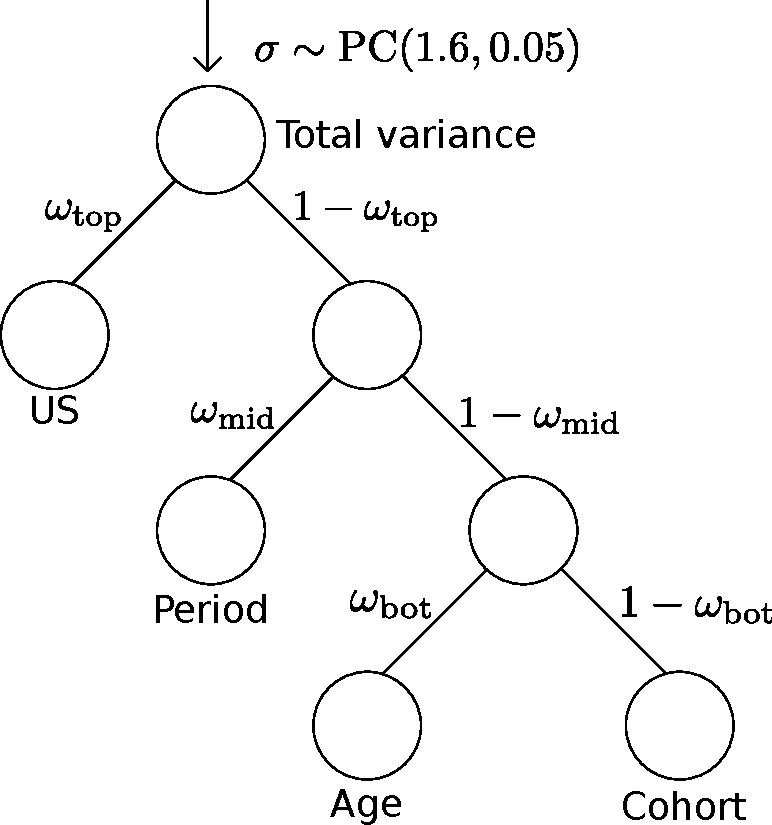
\includegraphics[width=0.6\textwidth]{Figures/Tree_some_annot.pdf}
    \caption{The hierarchical structure of the EK prior defined in Section \ref{section:application1:priorspecification}, visualized as a tree. The total variance, $\sigma^2$, is attributed to the top node, and then distributed to the unstructured (US), age, period, and cohort effects using the weight parameters $\omega_{\text{top}}$, $\omega_{\text{mid}}$, and $\omega_{\text{bot}}$ along the tree.}
    \label{figure:EK-tree}
\end{figure}

\subsubsubsection*{Alternative priors}
Naturally, a different expert on the field may disagree with the given expert knowledge. Therefore, the prior sensitivity of the model will be investigated to see how different priors affect the model. Since expert knowledge is available, an opposite or contradictory prior may be specified by doing the opposite of what is suggested by the expert knowledge. As we wish to compare the effects of different priors, preserving the same hierarchical structure is beneficial since we keep the same parameterization as the EK prior, and can compare the posteriors of $\omega_{\text{top}}$, $\omega_{\text{mid}}$, and $\omega_{\text{bot}}$. To create the "anti" prior to the EK prior while preserving the same structure, we simply swap the parameter specifying the median of the weight parameters at each split. That is, if the EK prior dictates a split attributing $30\%$ to one effect and $70\%$ to the other, this new prior then dictates that the first effect is attributed $70\%$ and the other $30\%$. The concentration parameter at each split is kept the same at $0.5$ to allow the same degree of uncertainty in the chosen median as in the EK prior. In addition, since the EK prior discourages overfitting to the structured effects by inducing shrinkage towards the unstructured effect, this new prior should induce shrinkage towards the structured effects. This "anti" prior will be dubbed the anti-EK prior.

In addition to the anti-EK prior, we may construct a prior that is unassuming in the hierarchical structure of the weight parameters. This is accomplished by attributing the total variance to the random effects using a single split with a Dirichlet(4) prior on the weight parameters. This way, the effects are considered equally important and have no enforced hierarchical structure outside the first split. The prior will simply be named the Dirichlet prior in the upcoming sections. Since the EK did not provide any information on the prior distribution of the standard deviation $\sigma$, it is kept identical as a $\text{PC}(1.6, 0.05)$ prior in all prior specifications. To bridge the gap in between the fully structured and unassuming prior structures, a prior structure with a split into structured and unstructured components was also tested, which uses a Dirichlet prior among the structured components. However, the prior structure was omitted since it achieved similar results as the other priors.

\subsubsection{Implementation in \texttt{R}}
\label{section:application1:prior-mmp}
The priors specified in Section \ref{section:application1:priorspecification} were implemented in \texttt{R} using the \texttt{makemyprior} package \citep{MMPPackage, MMP}. Details on the implementation and integration with \texttt{INLA} is found in Appendix \ref{appendix:implementation:prior}. The prior tree structure of the EK, anti-EK, and Dirichlet priors, visualized in the style of the graphical user interface in \texttt{makemyprior}, are shown in Figures \ref{figure:application1:EK}, \ref{figure:application1:antiEK}, and \ref{figure:application1:tree_dir} respectively. In these visualizations, the width of the arrows, along with the color intensity of the nodes, represent the prior weights given to the nodes, with higher intensity and width corresponding to higher weight. The arrow width is relative to each split, which reflects the weight attribution of the split, while the color intensity shows how much of the total variance is attributed to the effect. The dashed arrows indicate shrinkage away from the node being pointed to, reflecting the shrinkages discussed in Section \ref{section:application1:priorspecification}. The prior on the total standard deviation $\sigma$ for all prior specifications is shown in Figure \ref{figure:Application1:prior_var}. The priors on the weight parameters $\omega_{\text{top}}$, $\omega_{\text{mid}}$, and $\omega_{\text{bot}}$ are shown in Figures \ref{figure:application1:dir4}, \ref{figure:application1:priors_ek}, and  \ref{figure:application1:priors_anti_ek} for the Dirichlet, EK, and anti-EK priors respectively. 

\captionsetup[subfigure]{labelfont={bf,large}, font={large}, skip=1pt, margin=0cm, singlelinecheck=true}
%MMP EK and anti-EK structure 
\begin{figure}[h!]
    \centering
    \begin{subfigure}[b]{0.470\textwidth}   
        \centering 
        %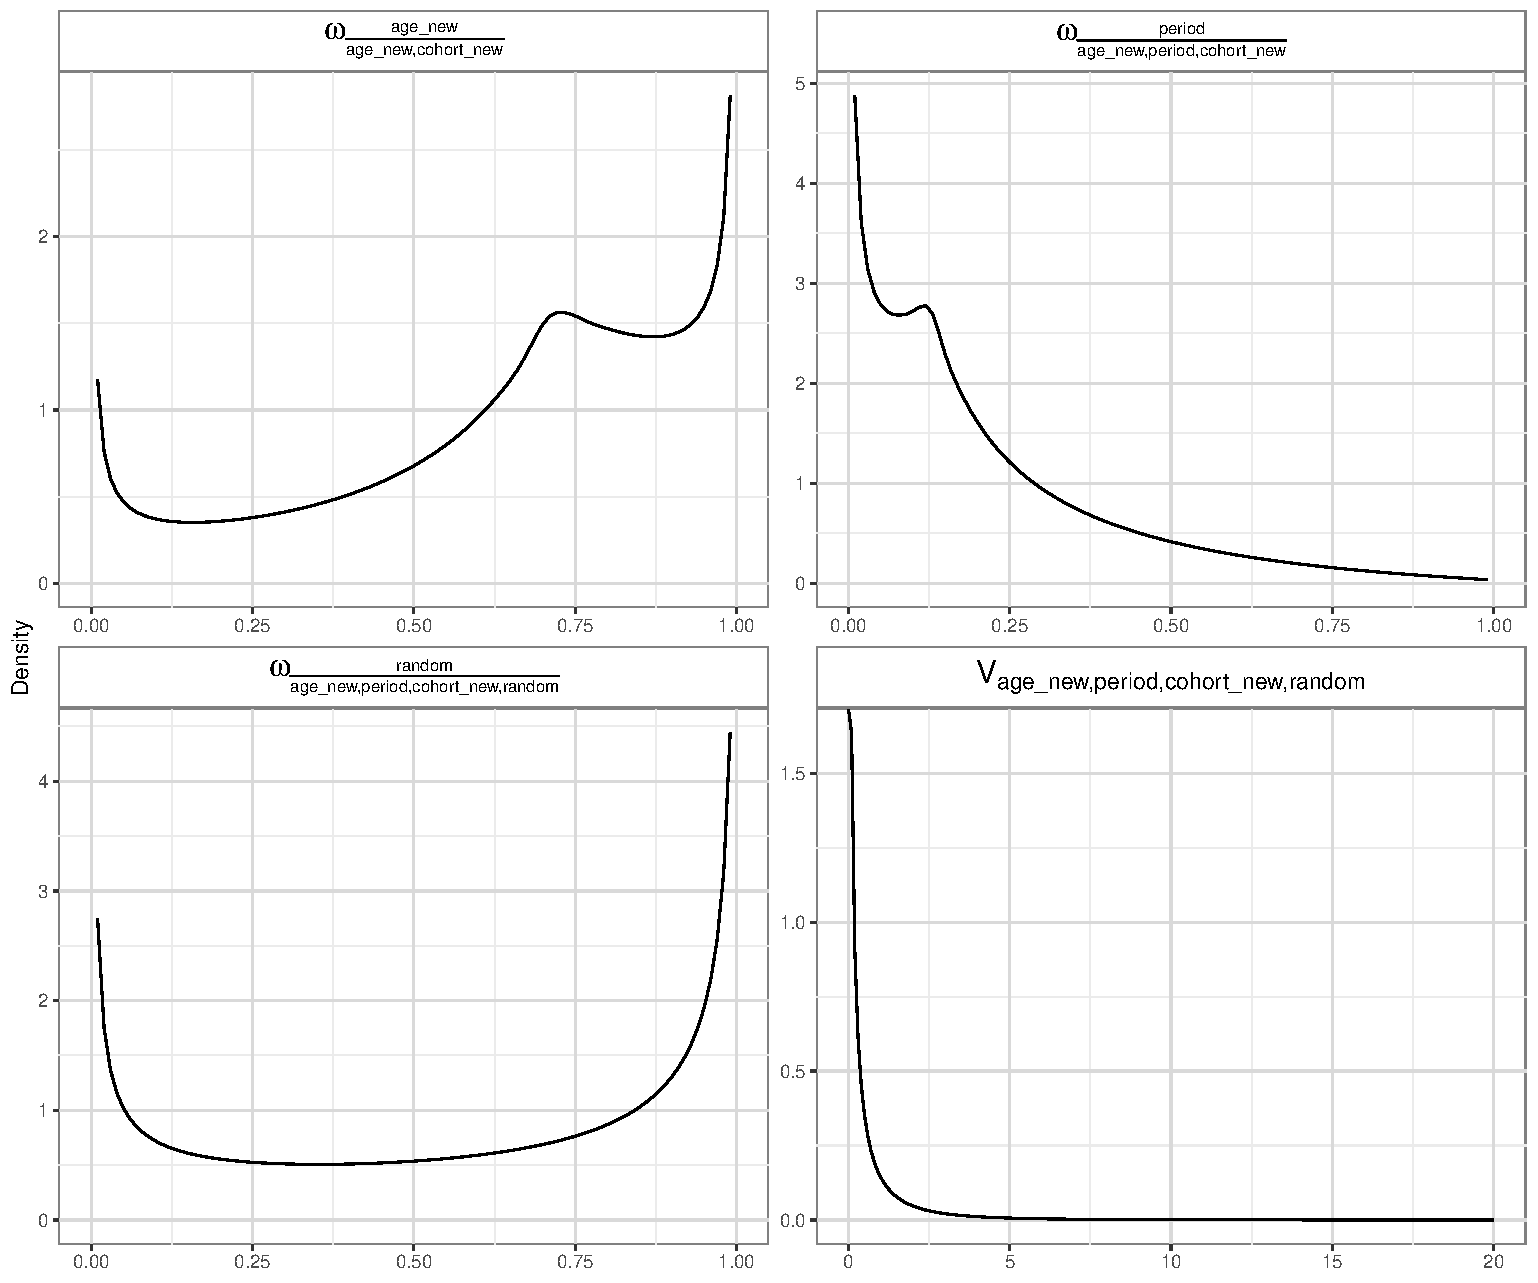
\includegraphics[width=\textwidth]{Figures/Prior_expert.png}
        
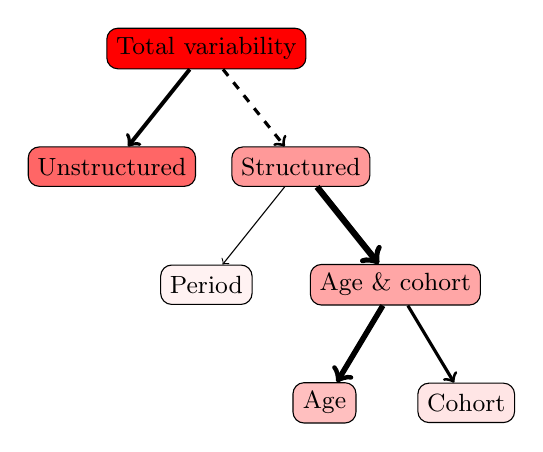
\begin{tikzpicture}[
    rounded corners,
    minimum height = 0.5cm, 
    minimum width = 0.8cm
]
\node[draw] (top) [fill = red!100] {{\color{black}\small Total variability}};
\node[draw] (gen) [below of = top, xshift = 1.2cm, yshift = -0.5cm, fill = red!40] {\small Structured};
\node[draw] (env) [below of = top, xshift = -1.2cm, yshift = -0.5cm, fill = red!60] {\small Unstructured};
\node[draw] (add) [below of = gen, xshift = -1.2cm, yshift = -0.5cm, fill = red!5] {\small Period};
\node[draw] (nonadd) [below of = gen, xshift = 1.2cm, yshift = -0.5cm, fill = red!35] {\small Age \& cohort};
\node[draw] (dom) [below of = nonadd, xshift = -0.9cm, yshift = -0.5cm, fill = red!25] {\small Age};
\node[draw] (epi) [below of = nonadd, xshift = 0.9cm, yshift = -0.5cm, fill = red!10] {\small Cohort};
% arrows
\path[->, every node/.style = {sloped, anchor = south, auto = false, anchor = mid, yshift = 0.15cm}]
(top) edge[line width = 0.5mm] node[] {} (env)
(top) edge[dashed, line width = 0.4mm] node[] {} (gen)
(gen) edge[] node[] {} (add)
(gen) edge[line width = 0.8mm] node[] {} (nonadd)
(nonadd) edge[line width = 0.7mm] node[] {} (dom)
(nonadd) edge[line width = 0.4mm] node[] {} (epi);

\end{tikzpicture}

        \caption[]%
        {{\small EK prior}}    
        \label{figure:application1:EK}
    \end{subfigure}
    \hfill
    \begin{subfigure}[b]{0.470\textwidth}   
        \centering 
        %\includegraphics[width=\textwidth]{Figures/Prior_anti.png}
        
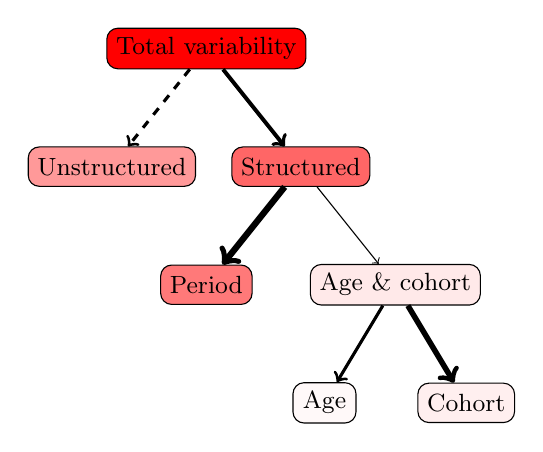
\begin{tikzpicture}[
    rounded corners,
    minimum height = 0.5cm, 
    minimum width = 0.8cm
]
\node[draw] (top) [fill = red!100] {{\color{black}\small Total variability}};
\node[draw] (gen) [below of = top, xshift = 1.2cm, yshift = -0.5cm, fill = red!60] {\small Structured};
\node[draw] (env) [below of = top, xshift = -1.2cm, yshift = -0.5cm, fill = red!40] {\small Unstructured};
\node[draw] (add) [below of = gen, xshift = -1.2cm, yshift = -0.5cm, fill = red!52.5] {\small Period};
\node[draw] (nonadd) [below of = gen, xshift = 1.2cm, yshift = -0.5cm, fill = red!8.5] {\small Age \& cohort};
\node[draw] (dom) [below of = nonadd, xshift = -0.9cm, yshift = -0.5cm, fill = red!2.4] {\small Age};
\node[draw] (epi) [below of = nonadd, xshift = 0.9cm, yshift = -0.5cm, fill = red!6.1] {\small Cohort};
% arrows
\path[->, every node/.style = {sloped, anchor = south, auto = false, anchor = mid, yshift = 0.15cm}]
(top) edge[dashed, line width = 0.4mm] node[] {} (env)
(top) edge[line width = 0.5mm] node[] {} (gen)
(gen) edge[line width = 0.8mm] node[] {} (add)
(gen) edge[] node[] {} (nonadd)
(nonadd) edge[line width = 0.4mm] node[] {} (dom)
(nonadd) edge[line width = 0.7mm] node[] {} (epi);

\end{tikzpicture}

        \caption[]%
        {{\small Anti-EK prior}}    
        \label{figure:application1:antiEK}
    \end{subfigure}
    \caption{Visualization of the attribution of variance in the \textbf{(a)} EK prior and \textbf{(b)} anti-EK prior defined in Section \ref{section:application1:priorspecification}. Greater arrow width corresponds to higher weight attribution in the split, and the dashed arrow indicates shrinkage away from the effect. The color intensity of the nodes correspond to the proportion of the total variance attributed to the effect.}
    \label{fig:result:prior}
\end{figure}

%MMP prior plots
\begin{figure}[h!]
    \centering
    \begin{subfigure}[b]{0.9\textwidth}
        \centering
        %\includegraphics[width=\textwidth]{Figures/Prior_dir.png}
        
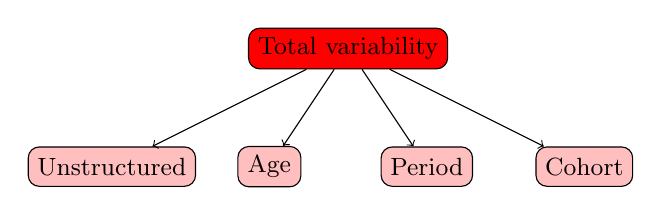
\begin{tikzpicture}[
    rounded corners,
    minimum height = 0.5cm, 
    minimum width = 0.8cm
]
\node[draw] (top) [fill = red!100] {{\color{black}\small Total variability}};
\node[draw] (US) [below of = top, xshift = -3cm, yshift = -0.5cm, fill = red!25] {\small Unstructured};
\node[draw] (Age) [below of = top, xshift = -1cm, yshift = -0.5cm, fill = red!25] {\small Age};
\node[draw] (Period) [below of = top, xshift = 1cm, yshift = -0.5cm, fill = red!25] {\small Period};
\node[draw] (Cohort) [below of = top, xshift = 3cm, yshift = -0.5cm, fill = red!25] {\small Cohort};
% arrows
\path[->, every node/.style = {sloped, anchor = south, auto = false, anchor = mid, yshift = 0.15cm}]
(top) edge[] node[] {} (US)
(top) edge[] node[] {} (Age)
(top) edge[] node[] {} (Period)
(top) edge[] node[] {} (Cohort)
;

\end{tikzpicture}

        \vspace{0.2cm}
        \caption[]{{\small Prior tree structure}}    
        \label{figure:application1:tree_dir}
    \end{subfigure}
    \vskip\baselineskip\vspace{-0.3cm}
    \begin{subfigure}[b]{0.35\textwidth}   
        \centering 
        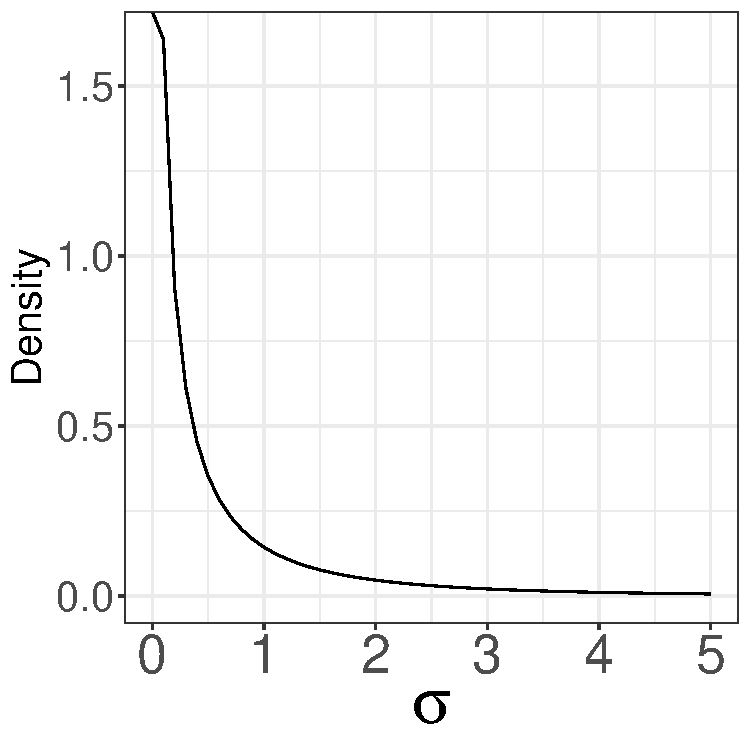
\includegraphics[width=\linewidth]{./Figures/prior_V.pdf}
        \caption[]{\small{$\text{PC}(1.6,0.05)$}}
        \label{figure:Application1:prior_var}
    \end{subfigure}
    \hspace{1cm}
    \begin{subfigure}[b]{0.35\textwidth}   
        \centering 
        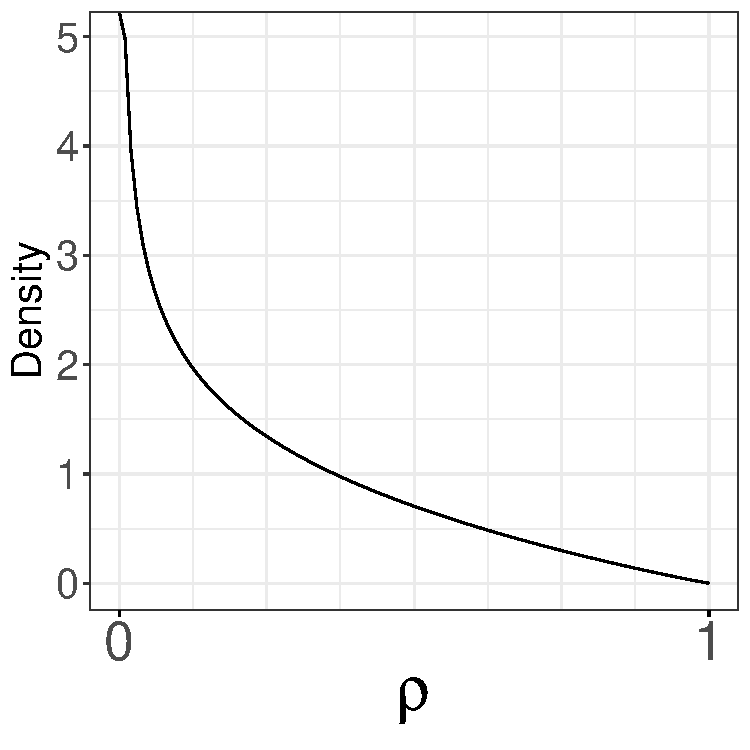
\includegraphics[width=\textwidth]{Figures/prior_dir4.pdf}
        \caption[]%
        {{\small Dirichlet(4)}}    
        \label{figure:application1:dir4}
    \end{subfigure}
    \caption{\textbf{(a)} The attribution of the total variance to the unstructured, age, period, and cohort effects in the Dirichlet prior defined in Section \ref{section:application1:priorspecification}. The equal color intensity of the nodes and uniform arrow width highlight the equal proportion of the total variance attributed to each effect. \textbf{(b)} Single weight parameter of a Dirichlet$(4)$ prior distribution. \textbf{(c)} The $\text{PC}(1.6,0.05)$ prior placed on the standard deviation in all prior structures specified in Section \ref{section:application1:priorspecification}. }
    \label{fig:application1:priors}
\end{figure}

%Prior of ek
\begin{figure}[h!]
    \centering
    \begin{subfigure}[b]{0.99\textwidth}
        \centering
        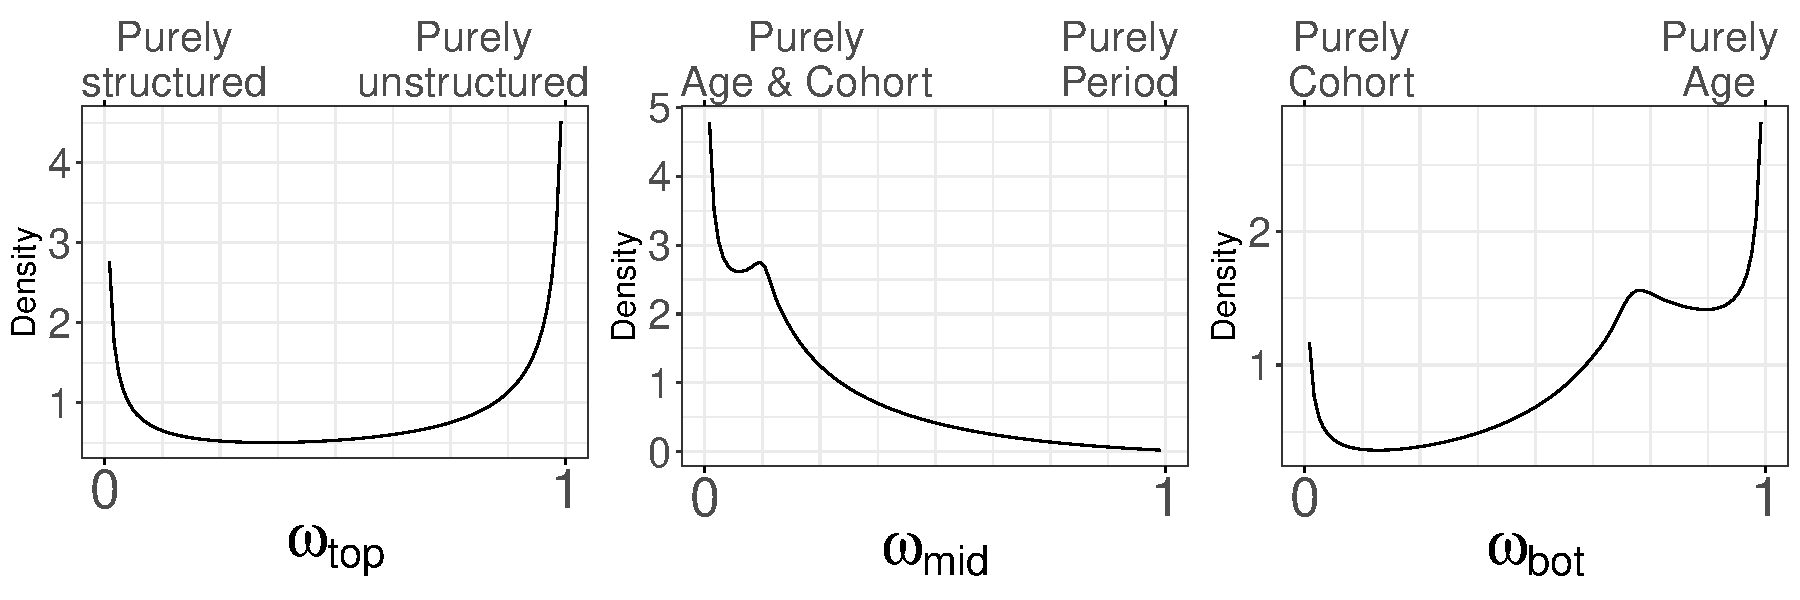
\includegraphics[width=\textwidth]{Figures/prior_rest.pdf}
        \caption[Network2]%
        {{\small EK prior}}    
        \label{figure:application1:priors_ek}
    \end{subfigure}
    \vskip\baselineskip\vspace{-0.5cm}
    \begin{subfigure}[b]{0.99\textwidth}   
        \centering 
        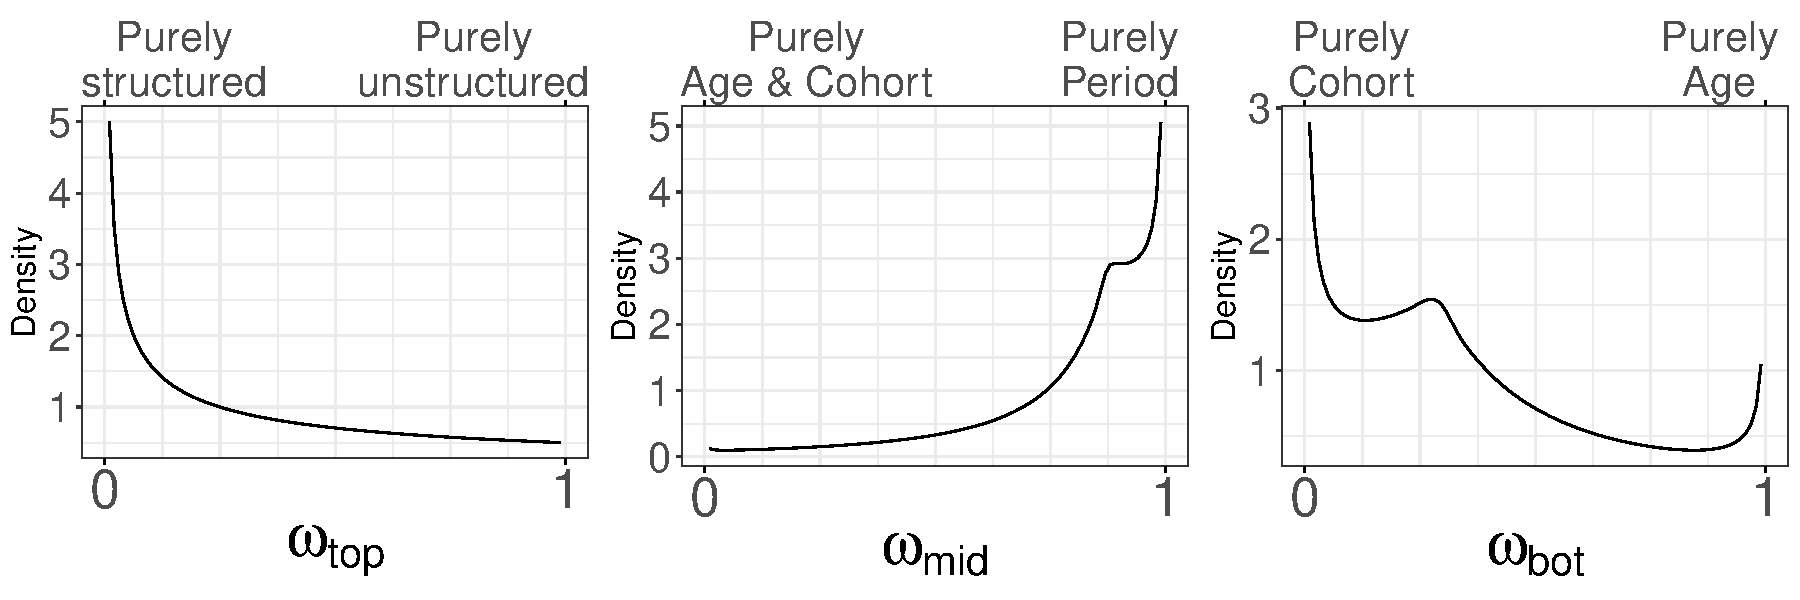
\includegraphics[width=\textwidth]{Figures/prior_rest_anti.pdf}
        \caption[]%
        {{\small Anti-EK prior}}    
        \label{figure:application1:priors_anti_ek}
    \end{subfigure}
    \caption{The prior distributions placed on the weight parameters $\omega_{\text{top}}$, $\omega_{\text{mid}}$, and $\omega_{\text{bot}}$ in \textbf{(a)} the EK prior and \textbf{(b)} the anti-EK prior, as defined in Section \ref{section:application1:priorspecification}. The location of the weight parameters along the prior tree structure is illustrated in Figure \ref{figure:EK-tree} with the same names, giving rise to the visualization in Figure \ref{fig:result:prior}.}
    \label{figure:application1:priors_weights}
\end{figure}


\FloatBarrier
\subsection{Posterior inference}
\label{section:application1:posteriorInference}
As mentioned in Sections \ref{section:Introduction} and \ref{section:Age-period-cohort-models}, a major consideration when using MAPC models is the issue of identifiability of the temporal effects. The random effects themselves are not identifiable due to their implicit linear dependence, but the linear predictor is identifiable, meaning we can use differences of the linear predictor to infer around the effect of stratification by educational attainment. In Section \ref{section:data:explorative}, we argued that BA+ level of attained education should serve as the baseline level for comparison. Using the definitions of the cross strata differences in Section \ref{section:APC-inference}, this corresponds to selecting BA+ to denote stratum $r_1$ in Equations \eqref{eqn:deltajk} and \eqref{eqn:deltak}. Moreover, in the presence of only one stratum-specific effect, we recall that when applying the exponential function to the cross strata differences, we interpret it as a ratio of odds. Should two stratum-specific effects be present, the interpretation changes to being the geometric mean of the odds ratio with respect to one temporal index, where the geometric mean is taken over the other temporal index. In practice, we do not compute the averaged differences which we interpret as the log-odds ratios, but rather define linear combinations of the stratum-specific intercepts and effects to be computed. By our Bayesian framework, each effect is now considered to be Gaussian a priori, meaning that our odds ratios also are considered Gaussian. Consequently, we may derive $95\%$ credible intervals in our inference. As for our given estimates, we will be using the median.  

The computation of these cross strata differences is easily performed in \texttt{INLA} by predefining linear combinations of the effects over the temporal indices to be computed using \texttt{inla.make.lincomb()}. An example of how these are provided is shown in Appendix \ref{appendix:implementation:lincombs}.

\FloatBarrier
\subsection{Model selection}
\label{section:model-selection}
With our methods and implementations in order, the only task left for a complete model specification is to complete the model choice by determining which effects should be shared between the different strata, and which effects should be stratum-specific. As mentioned in Section \ref{section:application1:priorspecification}, a requirement for the identifiability of the cross strata differences is that there is at least one shared effect and at least one stratum-specific effect. As a consequence of these requirements, we have $6$ candidate models from which we wish to select the one with the best fit. To rank the models, we use the logarithmic score, as well as WAIC and DIC (all described in Appendix \ref{section:disease-mapping:criteria}). All models are fitted using the EK prior.

\begin{table}[h!]
\centering
\begingroup\footnotesize\setstretch{1.2}

\begin{tabularx}{\textwidth}{llXXXXXX}
\hline
 &  & apC & aPc & aPC & Apc & ApC & \multicolumn{1}{c}{APc} \\ 
\hline
\nopagebreak log-score & \nopagebreak Female  & 2.673 & \textbf{ 2.669 } & 2.674 & 2.677 & 2.697 & 2.677 \\
 & \nopagebreak Male  & 2.500 & \textbf{ 2.497 } & 2.500 & 2.502 & 2.513 & 2.500 \\
\rule{0pt}{0.9\normalbaselineskip}WAIC & \nopagebreak Female  & 28228 & \textbf{ 28182 } & 28236 & 28270 & 28474 & 28265 \\
 & \nopagebreak Male  & 26394 & \textbf{ 26369 } & 26394 & 26417 & 26529 & 26403 \\
\rule{0pt}{0.9\normalbaselineskip}DIC & \nopagebreak Female  & 28221 & \textbf{ 28179 } & 28230 & 28263 & 28460 & 28259 \\
 & \nopagebreak Male  & 26392 & \textbf{ 26367 } & 26390 & 26411 & 26522 & 26400 \\
\hline 
\end{tabularx}\endgroup
 \caption{The achieved logarithmic score, WAIC, and DIC for each of the 6 candidate MAPC models, specified by different combinations of stratum-specific and shared age, period, and cohort effects. Shared effects are denoted with uppercase letters, and stratum-specific effects are denoted with lowercase letters. For each sex, the best model by each criterion is highlighted in bold.} \label{fig:model_selection_score}


\end{table}

The computed logarithmic score, WAIC, and DIC are shown in Table \ref{fig:model_selection_score} for all possible configurations of shared and stratum-specific effects, with the best models highlighted in bold for both sexes. Overall, the computed logarithmic scores, WAIC, and DIC are very similar within the male and female groups. The aPc model achieved the lowest logarithmic score for both sexes, and will therefore be interpreted in detail in the upcoming Section. From the lowest to highest scores, excluding the aPc model, are the apC, aPC, APc, Apc and ApC models. The scores of the top four models are very similar, and it would therefore be interesting to investigate the differences between these models.

\FloatBarrier
\subsection{Prior sensitivity analysis}
\label{section:application1:prior-sens}
\subsubsection{Methods}
\label{section:application1:prior-sens-motiv}
As this is a Bayesian analysis, we wish to carry out a prior sensitivity analysis using the EK, anti-EK, Dirichlet, and component-specific priors defined back in Section \ref{section:application1:priorspecification}. In addition, we investigate how models using joint prior specifications compare to models using component-specific priors, which is done by including a component-specific prior chosen unsubjectively as yet another contrast to the subjective prior elicited from EK.

We compare the effects of the priors on the model by comparing the posterior distributions of the estimated standard deviation $\sigma$, along with the weight parameters $\omega_{\text{top}}$, $\omega_{\text{mid}}$, and $\omega_{\text{bot}}$. Due to the different hierarchical structures of the Dirichlet and component-specific priors compared to the EK and anti-EK prior, direct and formal comparisons of the posteriors is difficult. Since we wish to compare the posteriors with respect to the EK prior, we estimate the posterior distributions of the weight parameters for the other priors at the levels of the EK prior. This also applies to the component-specific prior we also want to compare with. To remedy the issue of different structures, we sample the precision parameters from the posterior distributions and then transform them to match the levels of the hierarchical structure of the EK prior by Equations \eqref{eqn:omega_def}. While this does not reflect the structure of the used prior, it still allows for qualitative comparison to the EK prior, meaning we will be able to see if the different priors cause a different interpretation of the resulting model.

\FloatBarrier
\subsubsection{Results}
\label{section:application1:prior-sens-result}
Figures \ref{figure:Application1:s0_f}, \ref{figure:Application1:s1_f}, \ref{figure:Application1:s2_f}, and \ref{figure:Application1:s3_f} show the prior and posterior distributions of the standard deviation and mixing parameters, which are on the levels presented in the hierarchical decomposition prior tree in Figure \ref{figure:EK-tree} for the aPc model using data on female participants. To obtain the posterior distributions, 10,000 samples of the hyperparameters of each model were used. For the observed variance, shown in Figure \ref{figure:Application1:s0_f}, we observe that the posteriors are very similar despite the different prior specifications. In particular, it is interesting to note that the posterior using component-specific (CS) priors is also similar to the other models despite not sharing an identical prior at this level. On the first split of the tree, we see in Figure \ref{figure:Application1:s1_f} that the posterior places nearly all the weight of the mixing parameters on the temporally-structured components, and very little on the unstructured random effect. This is particularly interesting in the case of the model using EK, since this model facilitated shrinkage toward the unstructured random effect. Despite the shrinkage, the model clearly favors the structured components. In Figure \ref{figure:Application1:s2_f}, we also see that the different priors produce quite similar posteriors though with some slight differences. Here, the weight parameter clearly favors the age and cohort effects, i.e., the education-specific effects. For the last split, we once again see similar posteriors in Figure \ref{figure:Application1:s3_f}, with only small differences in the median estimate. Here we see that the median estimates are close to $0.5$, showing a preference to balance the education-specific effects. Overall, we see that the posterior distributions are very similar to each other, despite the use of very different priors. The equivalent plots using data on male participants is shown in Appendix \ref{appendix:figures} in Figures \ref{figure:Application1:s0_m} and \ref{figure:Application1:compare-plots_m}, and they exhibit the same behaviors as for the female data. In conclusion, the data is very informative, and therefore the models are not very sensitive to the prior.

\begin{figure}[!ht]
    \centering
    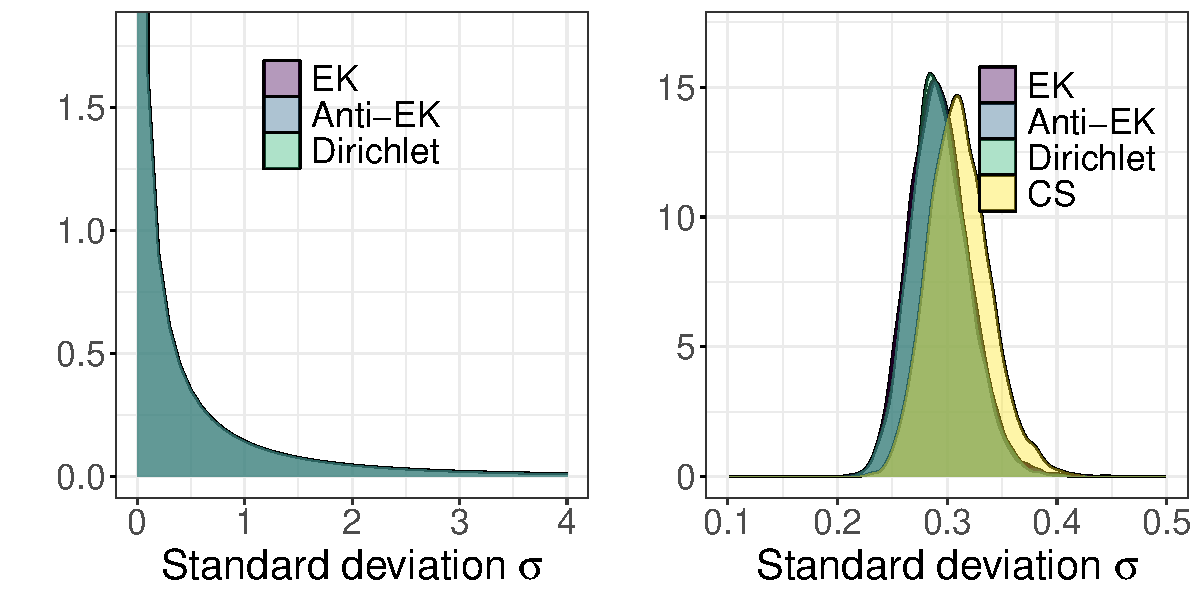
\includegraphics[width=0.8\textwidth]{Figures/compare_plots_s0_f.pdf}
    \caption{The (left) prior and (right) posterior distributions of the standard deviation in aPc models using female data along with the expert knowledge (EK), anti-EK, Dirichlet, and component-specific (CS) priors outlined in Section \ref{section:application1:prior}. }
    \label{figure:Application1:s0_f}
\end{figure}

\begin{figure}[!ht]
    \centering
    \begin{subfigure}[b]{0.8\textwidth}
        \centering
        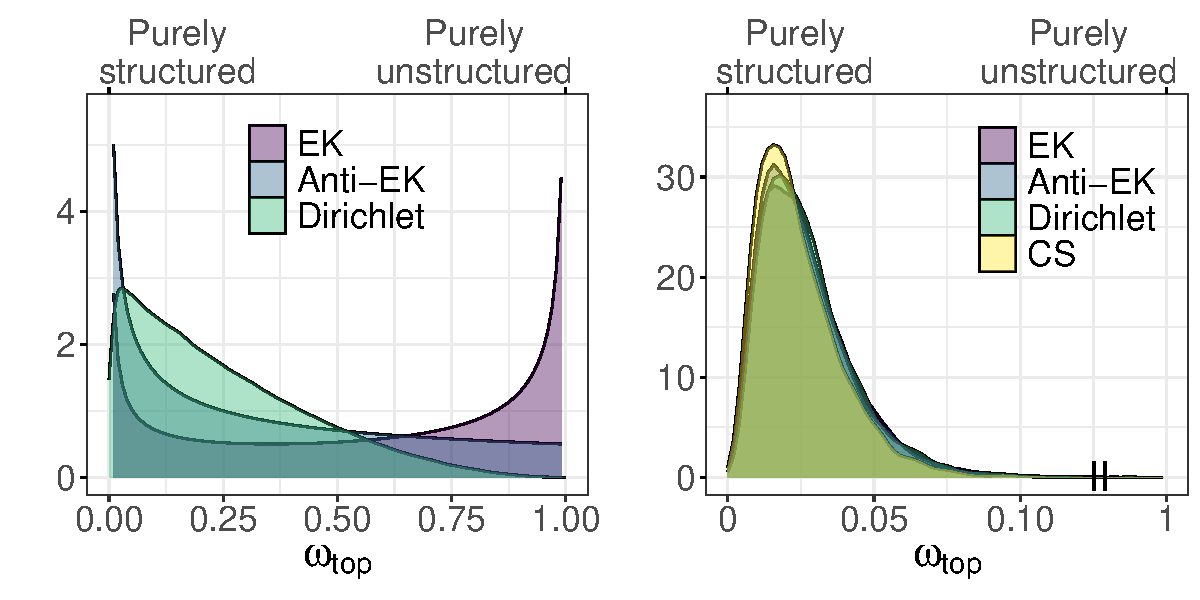
\includegraphics[width=\textwidth]{Figures/compare_plots_s1_f.pdf}
        \caption[Network2]%
        {{\small Top split}}    
        \label{figure:Application1:s1_f}
    \end{subfigure}
    \vskip\baselineskip\vspace{-0.5cm}
    \begin{subfigure}[b]{0.8\textwidth}   
        \centering 
        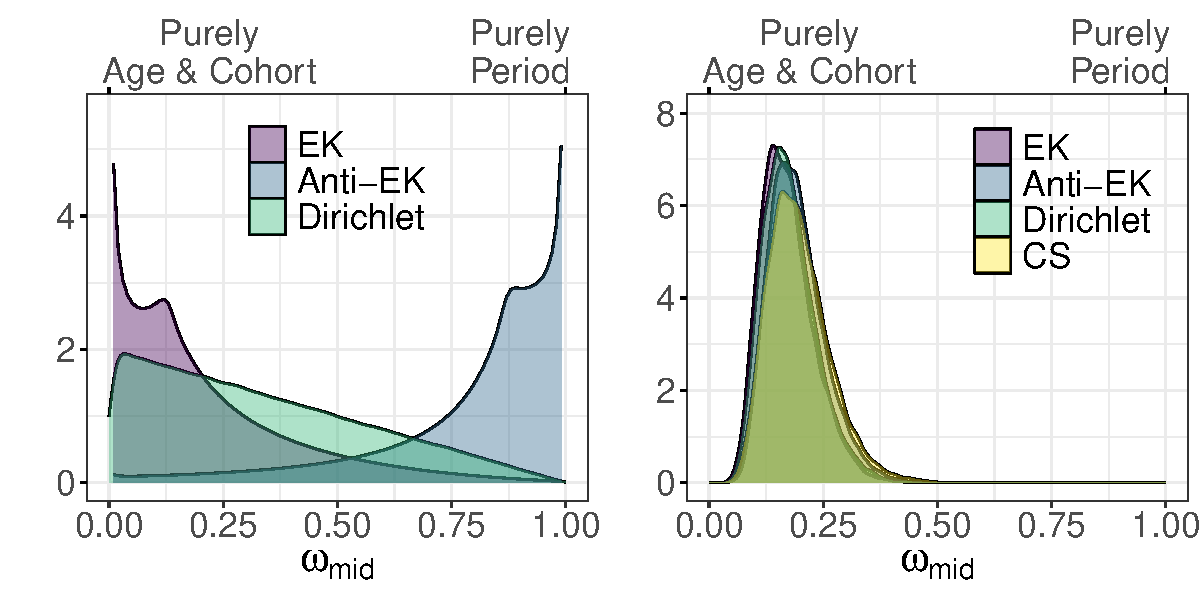
\includegraphics[width=\textwidth]{Figures/compare_plots_s2_f.pdf}
        \caption[]%
        {{\small Middle split}}    
        \label{figure:Application1:s2_f}
    \end{subfigure}
    \vskip\baselineskip\vspace{-0.5cm}
    \begin{subfigure}[b]{0.8\textwidth}   
        \centering 
        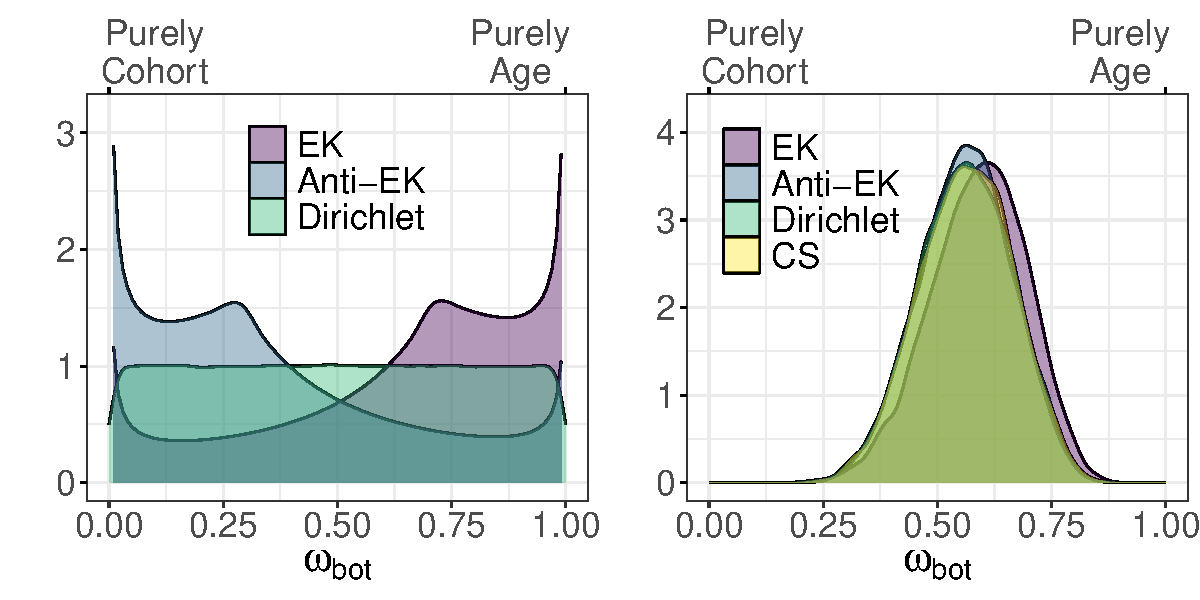
\includegraphics[width=\textwidth]{Figures/compare_plots_s3_f.pdf}
        \caption[]%
        {{\small  Bottom split}}    
        \label{figure:Application1:s3_f}
    \end{subfigure}
    \vspace{-0.2cm}
    \caption{The (left) prior and (right) posterior distributions of the mixing parameters at the \textbf{(a)} top, \textbf{(b)} middle, and \textbf{(c)} bottom levels in the hierarchical structure of the EK prior in aPc models using female data and the expert knowledge (EK), anti-EK, Dirichlet, and component-specific (CS) priors outlined in Section \ref{section:application1:prior}. }
    \label{fig:application1:compare-plots_f}
\end{figure}

\FloatBarrier
\subsection{Results}\label{section:application1:results}
\subsubsubsection*{Summary}
\vspace{-0.2cm}
For different levels of attained education, Figure \ref{figure:Application1:lincombs_best} shows the posterior medians of the odds ratio, as described in Section \ref{section:APC-inference}, over the relevant temporal indices in the aPc model using the EK prior for females and males separately, along with $95\%$ credible intervals. As these models incorporate education-specific age and cohort effects, the odds ratios over these two temporal indices are presented. As discussed in Section \ref{section:APC-inference}, the estimated odds ratios are with respect to the highest level of attained education, BA+. An odds ratio of $2$ implies that the odds are twice as large as in the group we compare with (BA+, in this case). A key observation is that in all figures, the estimated odds ratios are greater than $1$ everywhere, with credible intervals rarely including this value. By our discussion on the odds ratio in Section \ref{section:APC-inference}, this indicates a greater risk of back pain in all age groups and cohorts compared to BA+ level.

\captionsetup[subfigure]{font={bf,large}, skip=1pt, margin=0cm, singlelinecheck=false}

%Best model both sexes
\begin{figure}[h!]
    \centering
    \begin{subfigure}[b]{\textwidth}   
        \centering 
        \caption[]%
        {}    
        \label{figure:Application1:best_age_diff}
        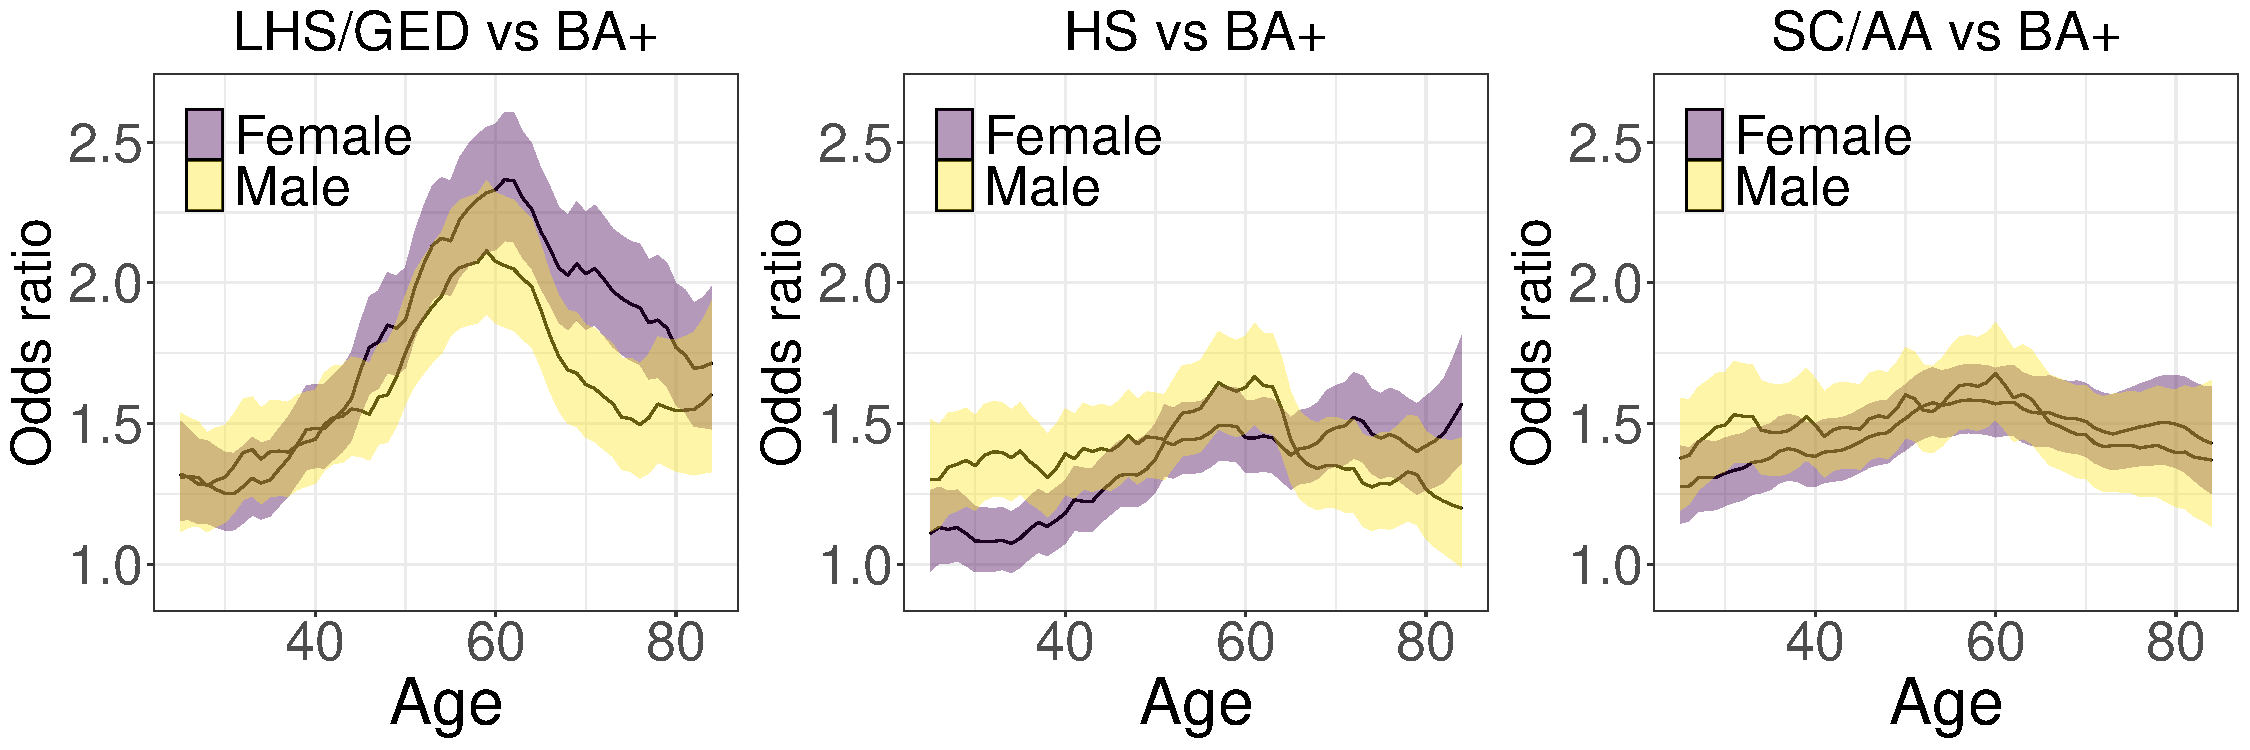
\includegraphics[width=\textwidth]{Figures/best_lincomb_age.pdf}
    \end{subfigure}
    \vskip\baselineskip\vspace{-0.3cm}
    \begin{subfigure}[b]{\textwidth}   
        \centering 
        \caption[]%
        {}    
        \label{figure:Application1:best_cohort_diff}
        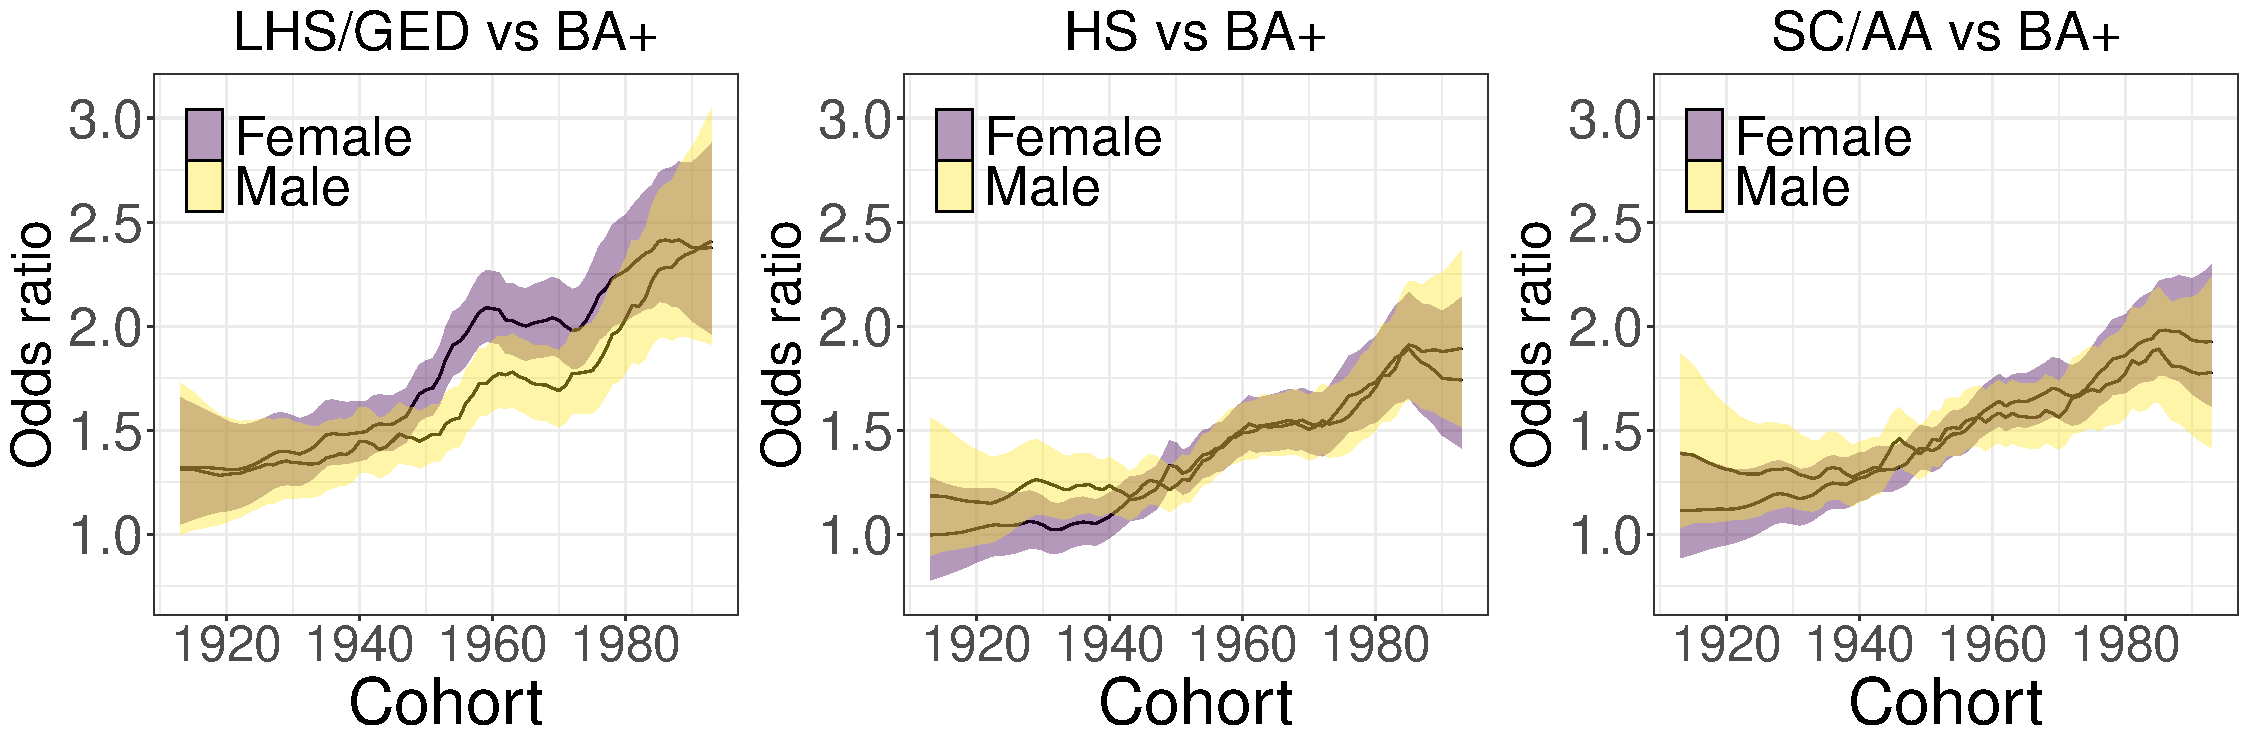
\includegraphics[width=\textwidth]{Figures/best_lincomb_cohort.pdf}
    \end{subfigure}
    \vspace{-0.2cm}
    \caption{Less than high school (LHS), high school (HS), and some college/associate of arts degree (SC/AA) levels of attained education with respect to bachelor or higher education (BA+), the posterior median odds ratio over \textbf{(a)} age and \textbf{(b)} cohorts, along with $95\%$ credible intervals. The trends are shown separately for males and females using the aPc model.}
    \label{figure:Application1:lincombs_best}
\end{figure}

\subsubsubsection*{Trends over age}
\vspace{-0.2cm}
In the estimated odds ratios over age, in Figure \ref{figure:Application1:best_age_diff}, we observe similar trends between males and females for LHS/GED and SC/AA levels of attained education. Meanwhile, some dissimilarities are observed for HS level of attained education. For LHS/GED level of attained education, we observe estimated odds ratios of around $1.3$ for both sexes in the youngest age groups, increasing steadily to $2.1$ for males and $2.35$ for females by age $60$, before declining to $1.6$ for males and $1.75$ for females by age $84$. This rising and falling (inverse V-shape) trend is also vaguely observed for SC/AA level of attained education, though with smaller differences between the sexes. For SC/AA level of attained education, the odds ratios are estimated around $1.25$ for females and $1.4$ for males at age $25$, increasing somewhat linearly to around $1.6$ for both sexes by age $55$ before declining to around $1.4$ to $1.45$ by age $84$. On the other hand, in the case of HS level of attained education, the trends visibly differ between the sexes. For males, we observe a less pronounced inverse V-shape trend, starting at $1.25$ at age $25$, increasing to $1.65$ by age $60$, before declining to $1.25$ again by age $84$. For females, the trend of odds ratios begins at $1.15$ at age $25$, increasing to around $1.4$ by age $50$, and remaining at this level until age $84$. In addition, we observe a particularly high risk of back pain among participants with LHS/GED levels of attained education, with odds ratios estimated as high as $2.35$ in some age groups. It is also interesting to note that female participants with LHS/GED level of attained education are more at risk than their male counterpart in age groups above $45$, while it is more even for the two other levels of education. 

%Over cohort
\subsubsubsection*{Trends over cohorts}
\vspace{-0.2cm}
In the estimated odds ratios over cohort, in Figure \ref{figure:Application1:best_cohort_diff}, we observe similar trends for both males and females, increasing with more recent cohorts in all levels of attained education. In the LHS/GED level of attained education, we observe odds ratio estimates of around $1.25$ for both sexes in the $1913$ birth cohort, increasing to $1.75$ for males and $2.05$ for females by the $1960$ birth cohort. The estimated odds ratios remain at these levels until the $1975$ birth cohort, after which the odds ratios begin to increase significantly to around $2.4$ for both sexes by the $1993$ birth cohort. For both the HS and SC/AA levels of attained education, we observe odds ratios of $1$ for females and $1.3$ for males in the $1913$ birth cohort, steadily increasing to around $1.85$ for both sexes by the $1985$ birth cohort. The estimated odds ratios remain at this level until the $1993$ birth cohort. As with the odds ratios over age, the estimated odds ratio is greater than $1$ almost everywhere, indicating that all participants with level of attained education lower than BA+ have a greater risk of backpain compared to the corresponding cohorts with BA+ level of attained education. We also observe higher risk particularly among participants with LHS/GED level of attained education, reaching odds ratios up to $2.4$.

%Top3 models female
\begin{figure}
    \centering
    \begin{subfigure}[b]{\textwidth}   
        \centering 
        \caption[]%
        {}    
        \label{figure:Application1:age_diff_f}
        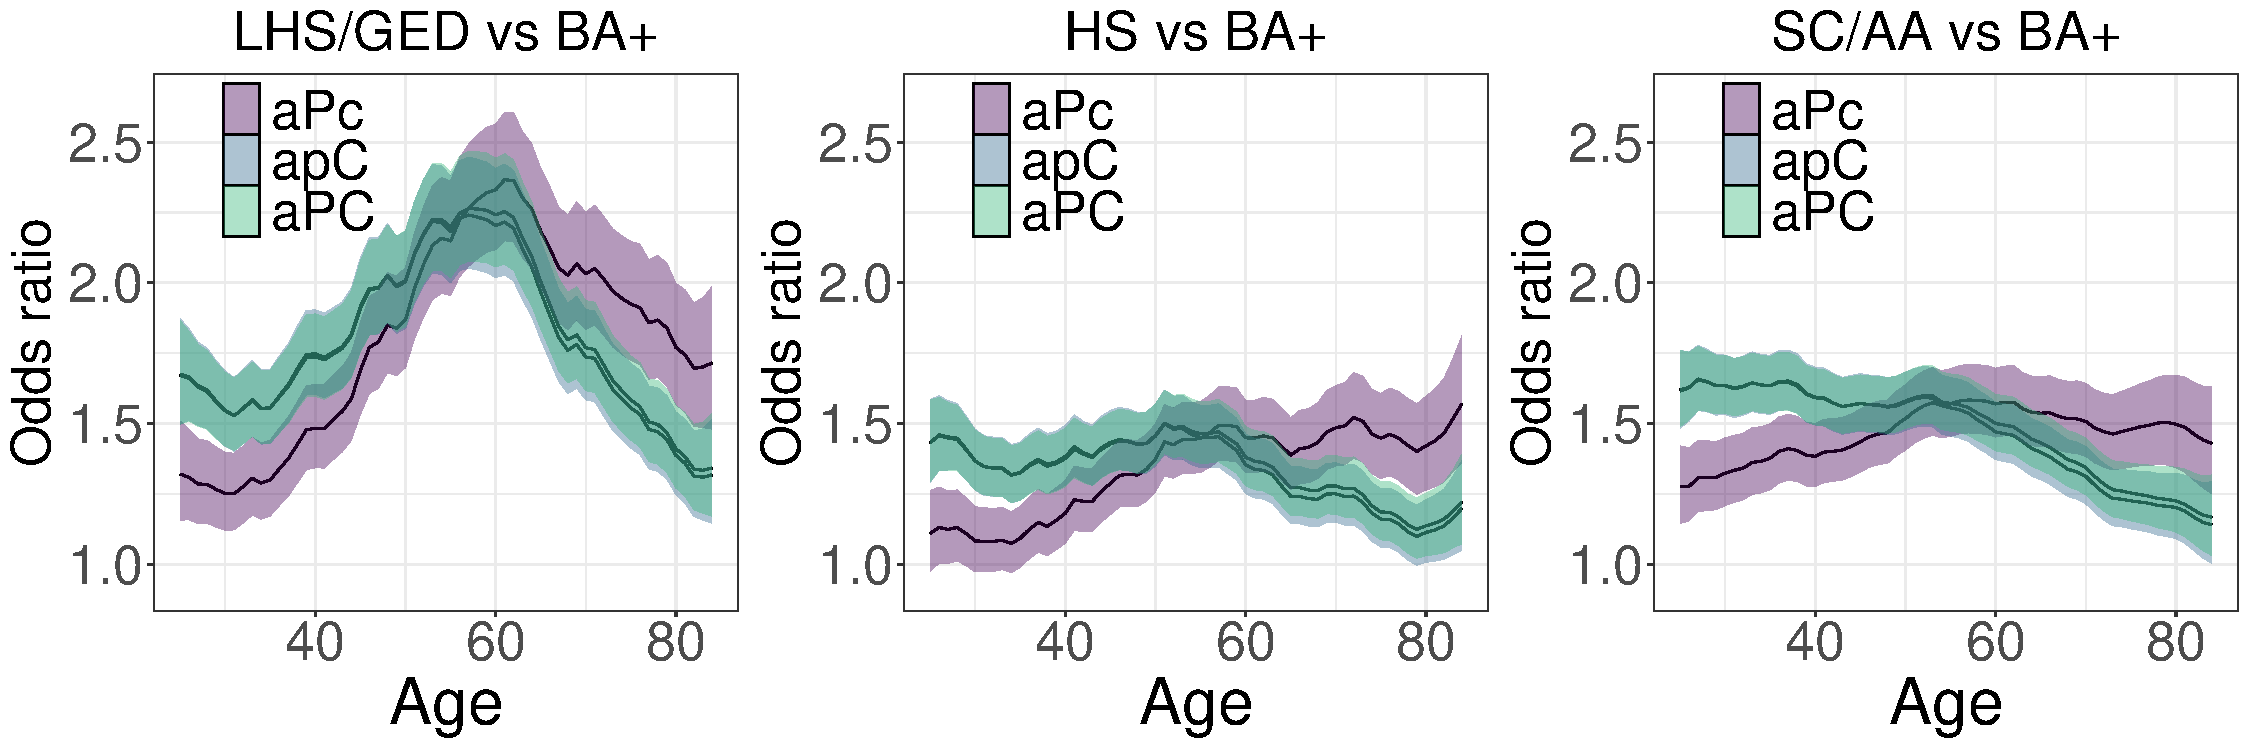
\includegraphics[width=\textwidth]{Figures/lincomb_age_f.pdf}
    \end{subfigure}
    \vskip\baselineskip\vspace{-0.3cm}
    \begin{subfigure}[b]{\textwidth}   
        \centering 
        \caption[]%
        {}    
        \label{figure:Application1:period_diff_f}
        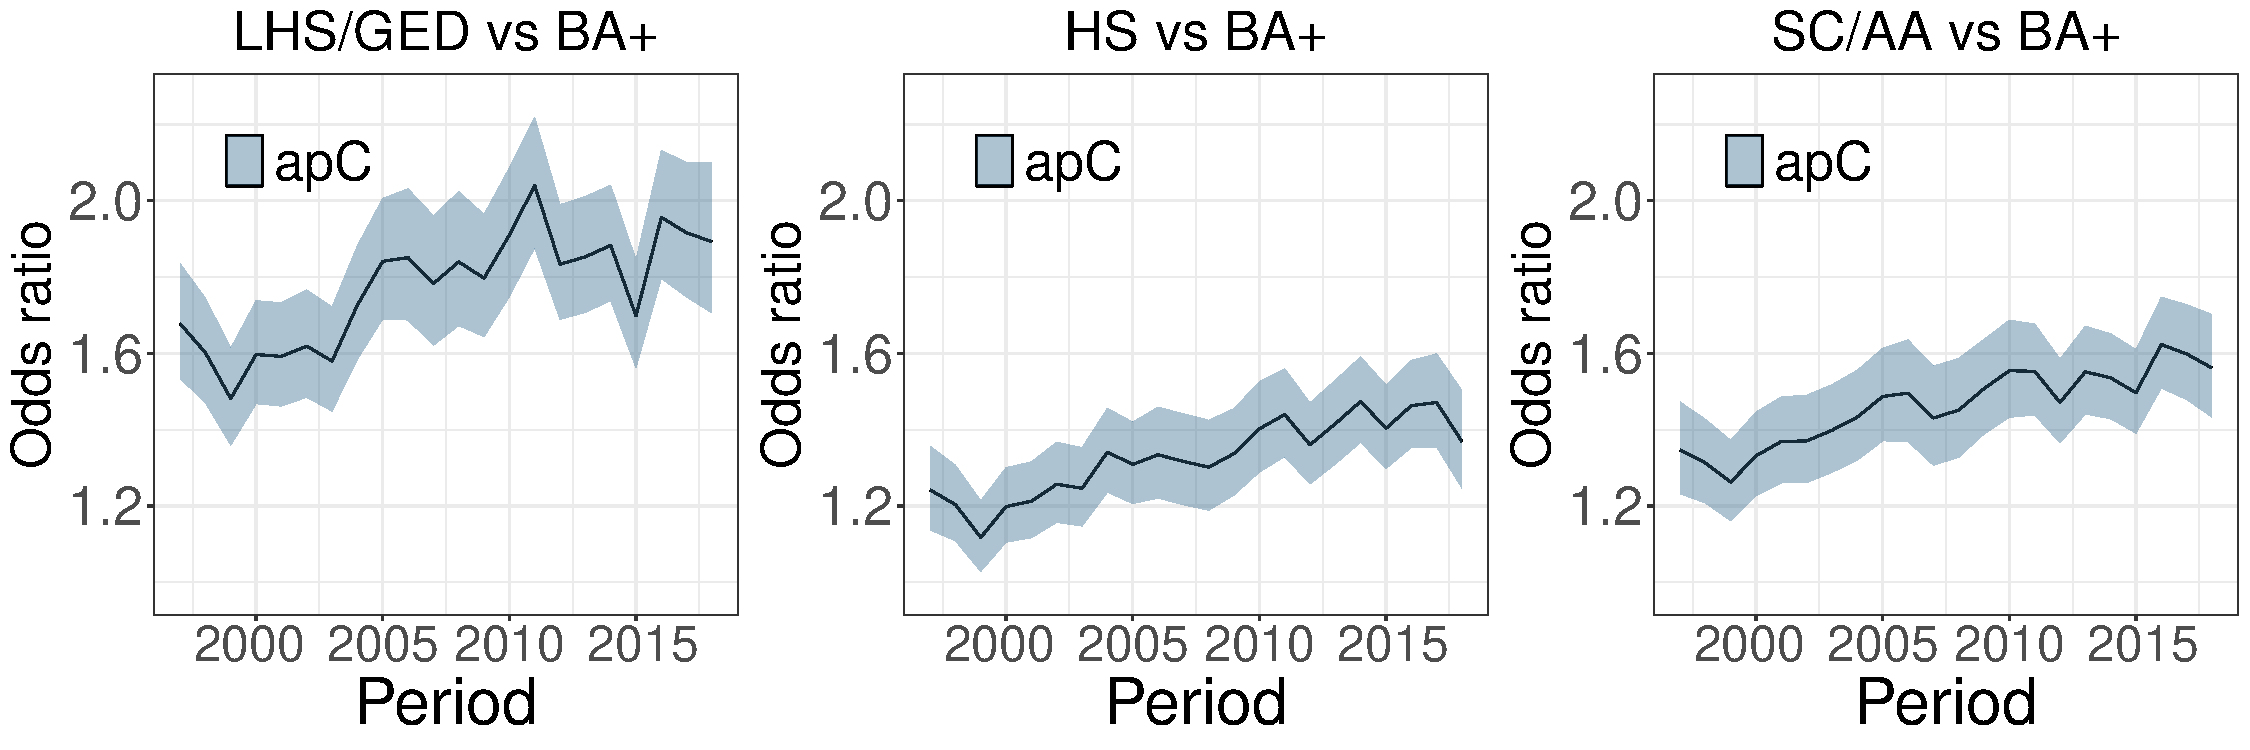
\includegraphics[width=\textwidth]{Figures/lincomb_period_f.pdf}
    \end{subfigure}
    \vskip\baselineskip\vspace{-0.3cm}
    \begin{subfigure}[b]{\textwidth}   
        \centering 
        \caption[]%
        {}    
        \label{figure:Application1:cohort_diff_f}
        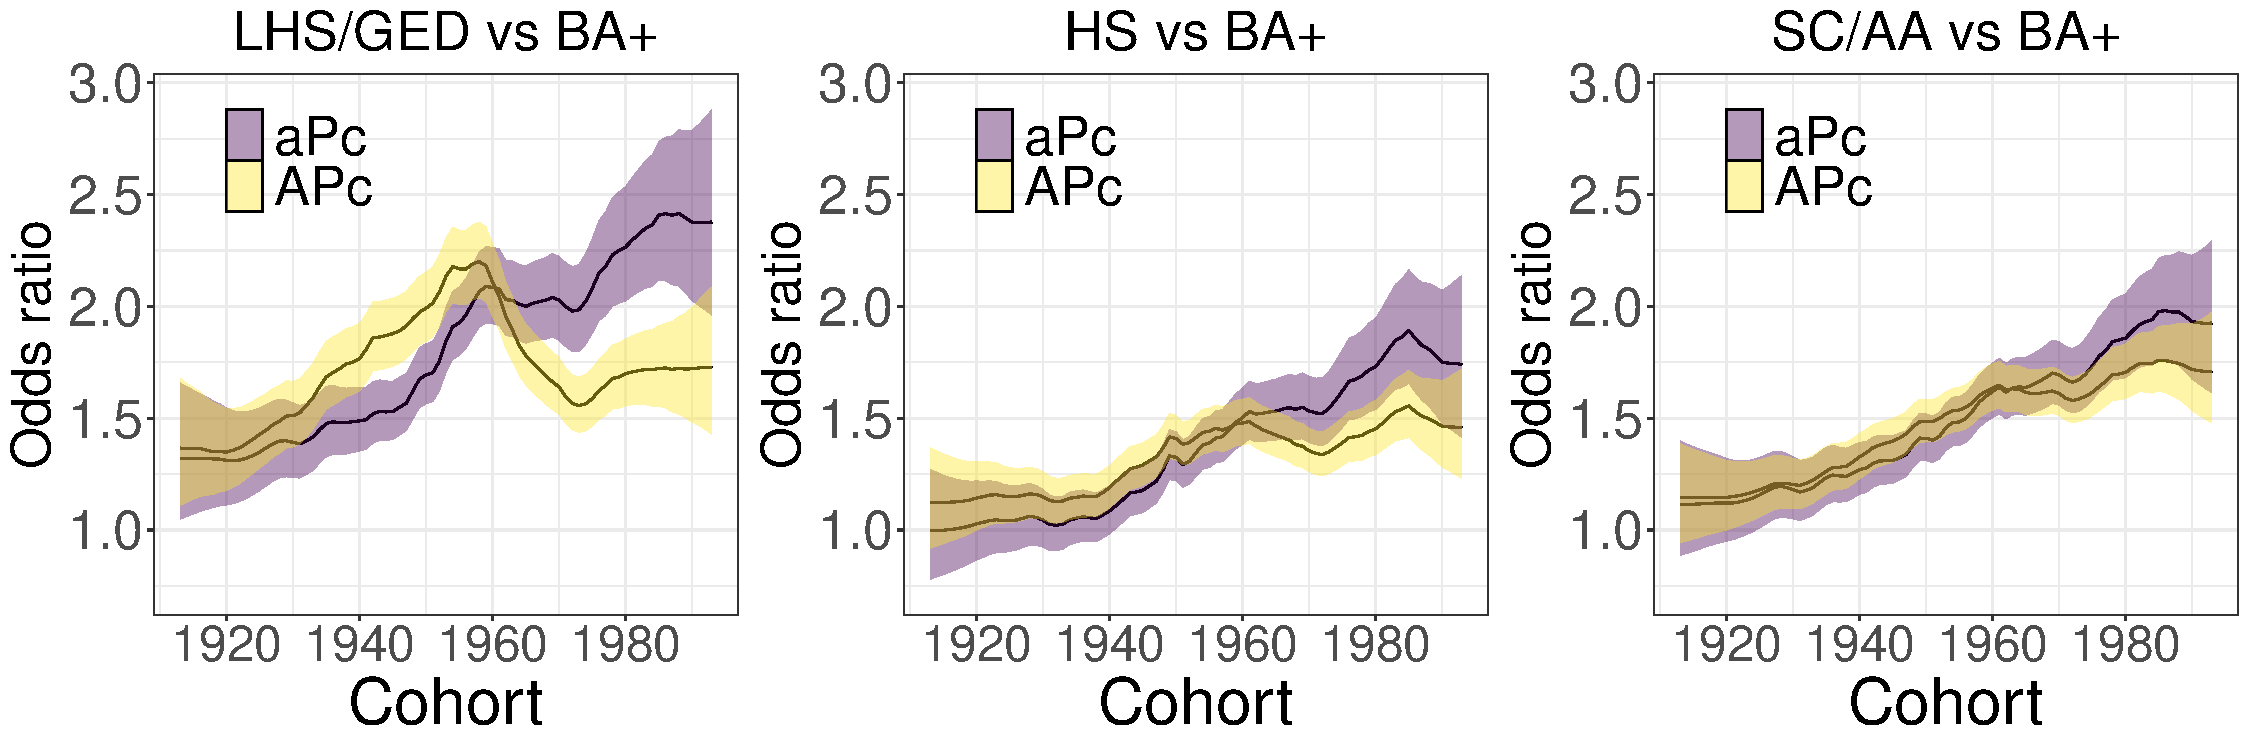
\includegraphics[width=\textwidth]{Figures/lincomb_cohort_f.pdf}
    \end{subfigure}
    \vspace{-0.3cm}
    \caption{For females with less than high school (LHS), high school (HS), and some college/associate of arts degree (SC/AA) levels of attained education with respect to bachelor or higher education, the posterior median odds ratio in the top four models by model selection over \textbf{(a)} age, \textbf{(b)} periods, and \textbf{(c)} cohorts, along with $95\%$ credible intervals.}
    \label{figure:Application1:lincombs_f}
\end{figure}

%Top3 models male
\begin{figure}
    \centering
    \begin{subfigure}[b]{\textwidth}   
        \centering 
        \caption[]%
        {}    
        \label{figure:Application1:age_diff_m}
        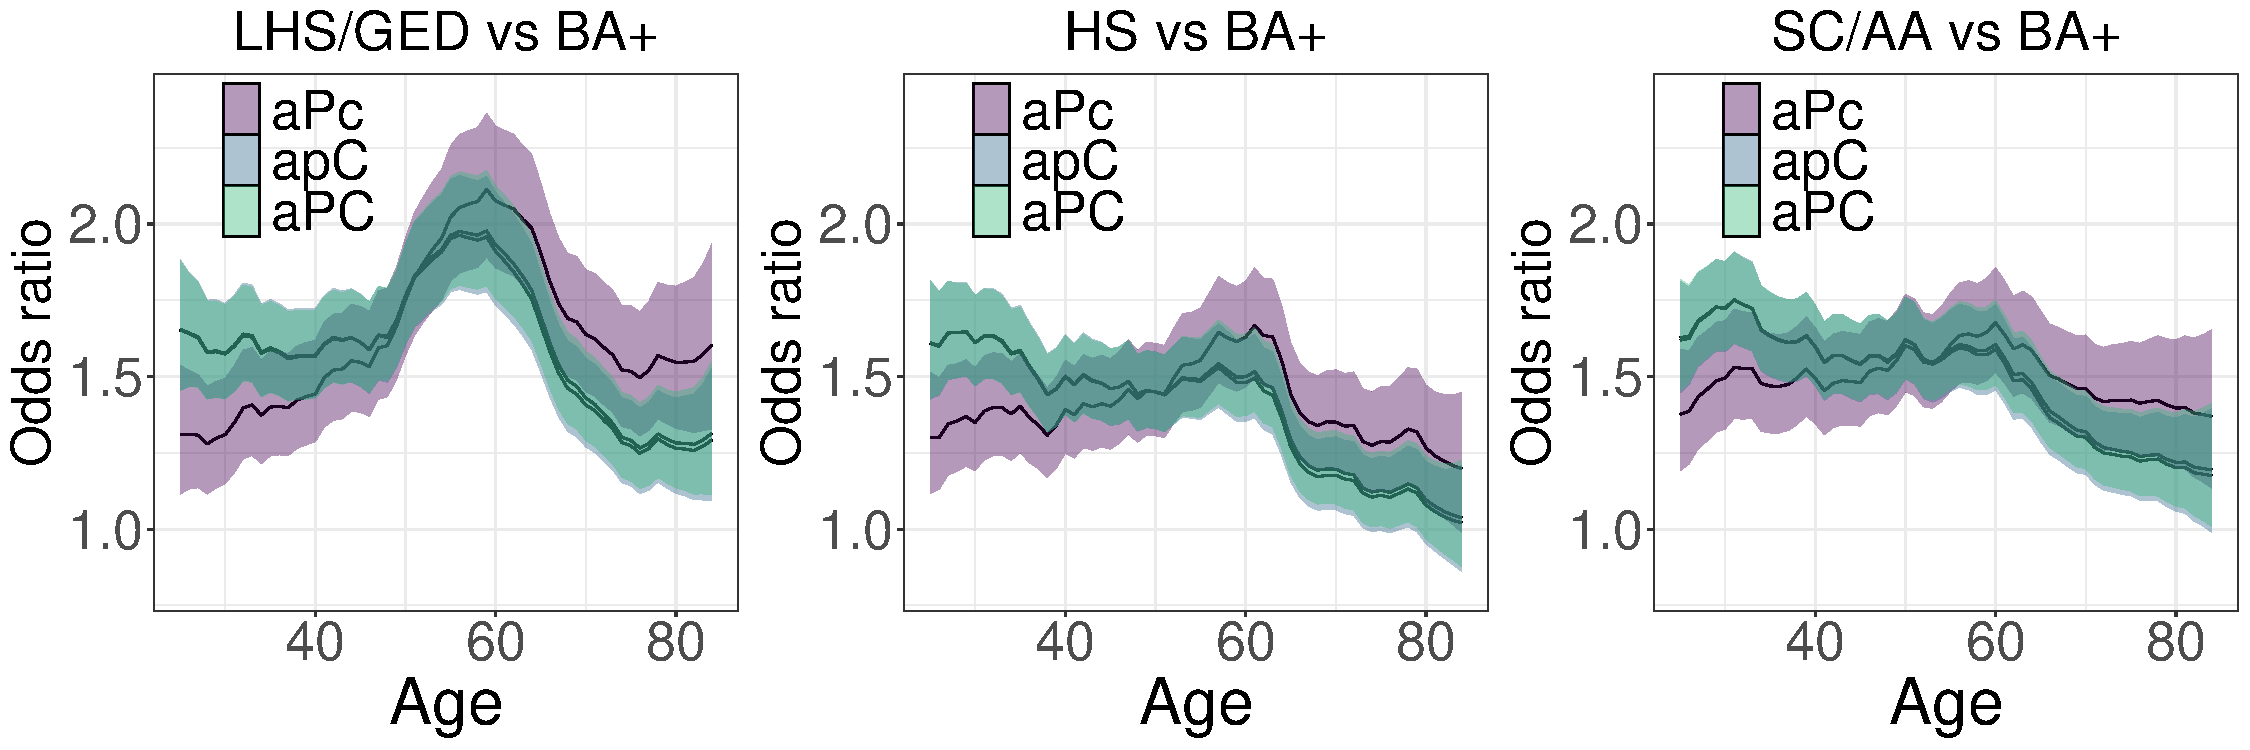
\includegraphics[width=\textwidth]{Figures/lincomb_age_m.pdf}
    \end{subfigure}
    \vskip\baselineskip\vspace{-0.3cm}
    \begin{subfigure}[b]{\textwidth}   
        \centering 
        \caption[]%
        {}    
        \label{figure:Application1:period_diff_m}
        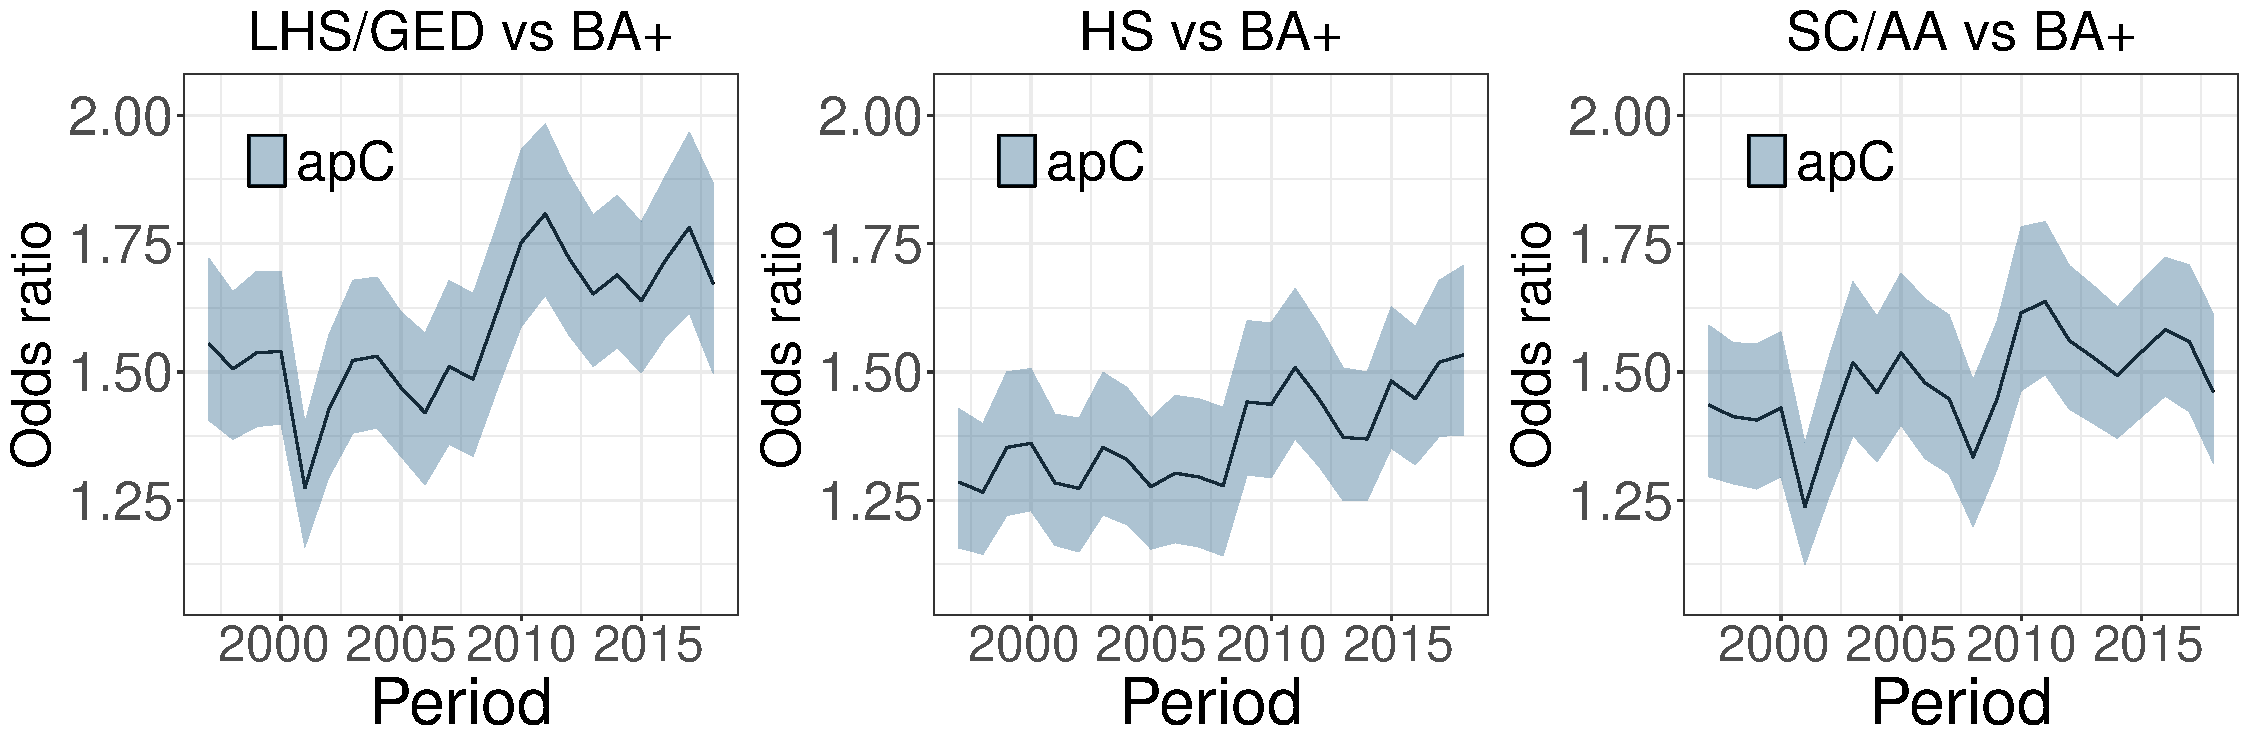
\includegraphics[width=\textwidth]{Figures/lincomb_period_m.pdf}
    \end{subfigure}
    \vskip\baselineskip\vspace{-0.3cm}
    \begin{subfigure}[b]{\textwidth}   
        \centering 
        \caption[]%
        {}    
        \label{figure:Application1:cohort_diff_m}
        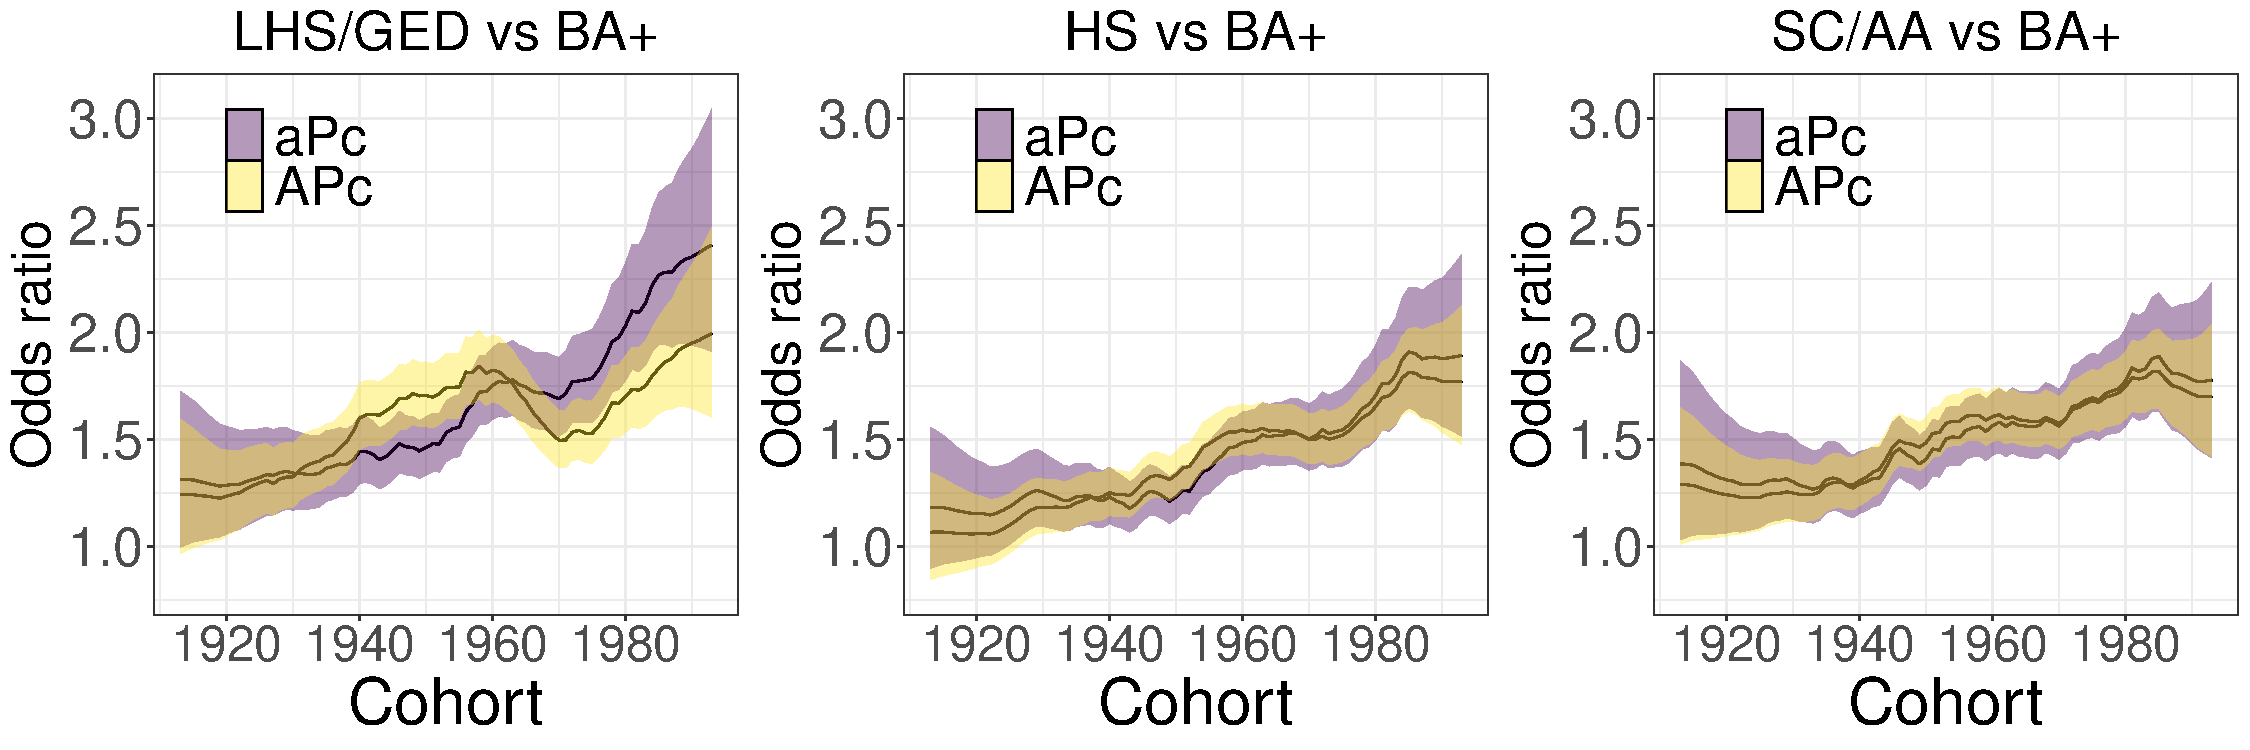
\includegraphics[width=\textwidth]{Figures/lincomb_cohort_m.pdf}
    \end{subfigure}
    \vspace{-0.3cm}
    \caption{For males with less than high school (LHS), high school (HS), and some college/associate of arts degree (SC/AA) levels of attained education with respect to bachelor or higher education, the posterior median odds ratio in the top four models by model selection over \textbf{(a)} age, \textbf{(b)} periods, and \textbf{(c)} cohorts, along with $95\%$ credible intervals.}
    \label{figure:Application1:lincombs_m}
\end{figure}

%Multiple models results
\subsubsubsection*{Top four models}
\vspace{-0.2cm}
The posterior medians of the odds ratio in the top four models chosen by model selection in Section \ref{section:model-selection} along with $95\%$ credible intervals are shown in Figure \ref{figure:Application1:lincombs_f} for female data and Figure \ref{figure:Application1:lincombs_m} for male data. Figures \ref{figure:Application1:age_diff_f} and \ref{figure:Application1:age_diff_m} show the estimated odds ratios over age in the aPc, apC, and aPC models. Over age, the estimated trends for the apC and aPC models are nearly identical, and are noticeably different from the trends estimated in the aPc model. As these are different models in terms of how the effects are modelled, some variation in the estimated trends is expected. It is interesting, however, to see that the model with stratum-specific cohort effects arrives at significantly different estimates than the models without. Meanwhile, due to the similar estimated trends in the apC and aPC models, it seems that stratification of the period effects cause little change in the estimates. Taken together, it seems that the combination of stratum-specific age and cohort effects is what affects the estimated trends the most. As for the odds ratio over period, in Figures \ref{figure:Application1:period_diff_f} and \ref{figure:Application1:period_diff_m}, we only have one model using a stratum-specific period effect (the apC model), meaning we have no models to compare the estimated trend with. Nevertheless, it is interesting to see that the estimated odds ratio trend over periods is generally slightly increasing with some fluctuation in all levels of attained education. Figures \ref{figure:Application1:cohort_diff_f} and \ref{figure:Application1:cohort_diff_m} show the estimated odds ratios over cohorts in the aPc and APc models. As we saw with these two models over age, the aPc and APc models arrive at noticeably different estimates of the odds ratios, particularly for LHS/GED level of attained education, where the odds ratios appear to decrease significantly between the $1960$ and $1970$ birth cohorts. This effect is quite drastic in the models using female data. Over the other levels of attained education, however, we see similar trends in both models for both sexes. Again, these differences indicate that different combinations of stratification by educational attainment in the age and cohort effects greatly influence the estimated trends, which underscores how crucial the age and cohort effects are when it comes to explaining the data.

\FloatBarrier
\subsection{Discussion}\label{section:Application1:Dicussion}
\subsubsubsection*{Summary}
\vspace{-0.2cm}
In this thesis so far, we have constructed a prior tailored for a Bayesian MAPC model, which incorporates provided sociological expert knowledge, as inspired by the approach used by \cite{IngeborgGenetics}, by using PC priors \citep{PC-priors}, together with the intuitive structure of HD priors \citep{Jointprior}. Moreover, the prior sensitivity analysis showed that the MAPC model in this application does not seem to be sensitive to the prior, since priors incorporating the "anti" expert knowledge showed similar results. From the model selection, models with different specifications of shared and stratum-specific age, period, and cohort effects were tested, and the model scores were found to be similar, though the aPc model appears to be slightly favored for both sexes. Then, interpreting the estimated cross strata differences in the aPc model as odds ratios (according to Section \ref{section:APC-inference}), the estimated odds ratios display clear temporal trends over age and cohorts. The estimated odds ratios among participants in all levels of attained education is generally increasing with age and more recent cohorts compared to that for the BA+ level, with substantially higher estimates among participants with the LHS/GED level of attained education. Consequently, our analysis shows rising differences in risk of back pain over age and cohorts, with some age groups and cohorts experiencing $2.5$ times as large odds of backpain as the corresponding group with BA+ level of attained education. Lastly, we examined the differences in the estimated trends between models using different combinations of shared and stratum-specific age, period, and cohort effects.

%Model selection, how robust
\subsubsubsection*{Model selection}
\vspace{-0.2cm}
The model selection performed in Section \ref{section:model-selection} revealed a preference for the aPc model in all scoring criteria when using male and female data separately. Interestingly, the computed logarithmic scores are very similar for all models, indicating that there is not a strong preference for any model overall. By looking at our secondary criteria, WAIC and DIC, we also see that there is a slight preference for the aPc model, though other models again achieve comparable scores. As a consequence, relying solely on the model scores for model selection is unadvised. Though in this case, the marginally-better model happened to have education-specific age and cohort effects, which also were the effects indicated to have high importance by the EK. Therefore, this model naturally becomes the preferred model for further analysis in either case. As we saw with the prior sensitivity analysis, the posteriors did not change much when using different priors, meaning we would most likely still select the aPc model with a different prior specification. Slight variations in the data, on the other hand, could have resulted in a different preferred model due to the similarly achieved scores. 

%Shortly about GED disparity in general
\subsubsubsection*{Disparities in the LHS/GED educational group}
\vspace{-0.2cm}
In Section \ref{section:application1:results}, the estimated temporal trends in the aPc model revealed heterogeneous time trends across different levels of attained education for males and females separately. In both temporal trends, we observe rising differences compared to BA+ level of attained education, with estimates of the odds ratio greater than one almost everywhere. As discussed in Section \ref{section:APC-inference}, larger odds ratio indicates that the risk of back pain is heightened among participants with the given level of attained education, in comparison to the participants with BA+ level of attained education. Since this odds ratio is almost always greater than one, it indicates an overall disparity in health outcomes compared to BA+ level. In addition, we saw over both age and cohorts that participants with LHS/GED level of attained education is particularly at risk, with larger estimated odds ratios than the corresponding age groups and cohorts with HS and SC/AA levels of attained education. This overall disparity compared to BA+ level, and particular disparity for LHS/GED level of attained education has been observed already in other studies \citep{GEDdisparity}, which is reassuring and solidifies our grounds for temporal analysis and interpretation of the resulting trends.

%Age inverse V-shape
\subsubsubsection*{Trends over age}
\vspace{-0.2cm}
By our results, we elaborated upon these disparities in health by examining them in a temporal context, from which we observed similar trends over age in certain levels of attained education. In the models using male data, we saw an inverse V-shaped trend in all levels of attained education. The increasing risk of back pain with age makes sense since the age effect captures cumulative exposure to risk, as discussed in Section \ref{section:lexis}. What is interesting to see is that the risk of back pain appears to decrease noticeably compared to BA+ level after age $60$. The decrease could be attributed to multiple potential reasons, and the exact causes and explanations are better left to sociologists. However, one possible partial explanation could be due to selective mortality \citep{beckett2000converging, house1990age, lynch2003cohort}. The older age groups could consist of the survivors of their generation, meaning they are the ones of their generation who survived to old age. Thus, we only have observations on participants with exceptionally good health, since those with worse health may have already died before reaching old age. In turn, the health outcomes of these survivors may appear more in line with the health outcomes of participants with BA+ level of attained education. Therefore, the decrease could be, at least in part, due to higher mortality in the other levels of education compared to BA+ level. This could also be particularly the case for LHS/GED level of attained education, in which we observe the greatest decrease and disparities post age group $60$. Several factors are likely at play here, and further interpretation and investigation by experts would be beneficial in explaining the observed temporal trends.

%Difference between female and male estimates
\subsubsubsection*{Comparison between males and females}
\vspace{-0.2cm}
In our estimated trends, both similarities and differences were observed by sex. Over cohorts, the estimated trends are very similar in shape and magnitude, though for participants with LHS/GED level of attained education, we observe higher estimates for males than females between the $1940$ and $1980$ birth cohorts. Overall, these trends over cohorts are very similar in both sexes, indicating a similar evolution of socioeconomic factors over cohorts for both sexes, within all levels of attained education. Over age, substantially higher risk was observed among females compared to males with LHS/GED level of attained education. Moreover, the estimated trends were quite different for HS level of attained education. In females, we saw an increasing trend between ages $25$ to $50$, after which it became stagnant, while for males we observe an increasing trend until age $60$, after which it declines. The exact causes of these observed differences, particularly for the younger ages, are difficult to gauge at, and once again calls for sociologists to interpret.

%Alternative models results
\subsubsubsection*{Trends in alternative models}
\vspace{-0.2cm}
When considering the alternative, similar scoring models to the aPc models, we saw that the estimated trends over both age and cohorts differ noticeably depending on what effects are stratified by educational attainment. Interestingly, in alternative models to the aPc model, we still observe the inverse V-shape trend over age, though with an even more significant decrease in risk after age $60$. Interestingly, the two different trends in each group of education over age appear to be rotations of each other. However, this is not a cause for concern, as the models are inherently distinct from each other due to the different specifications of shared and stratum-specific effects. Moreover, over cohorts with LHS/GED level of attained education, we observe strange behaviors in the alternative model with a sudden dip in risk between the $1960$ and $1970$ birth cohort, in particular for females. While we see differences in the estimated trends over cohorts for all levels of education, none of them are as great and as abrupt as for LHS/GED level of attained education, calling for further investigation on the trends for this level of attained education. In all models, the estimated odds ratios are still greater than one everywhere, meaning that the overall disparity in health for all levels of attained education compared to BA+ level remains readily apparent. Coupled with the small differences in model scores, great care should be taken when selecting a model to analyse, and the context of which effects are stratified by education should be taken into account in the interpretation. 

%Prior sensitivity results
\subsubsubsection*{Prior sensitivity}
\vspace{-0.2cm}
From the prior sensitivity analysis in Section \ref{section:application1:prior-sens-result}, the aPc model chosen by model selection shows remarkable similarities when fitted with different priors. The models largely gravitate towards placing the posterior mass of the weight parameters in the same vicinity, meaning that the models do not appear to be sensitive to the prior. Moreover, the models distribute most of the variance to the age and cohort effects, which also happen to be the stratum-specific effects, which underscores the importance of the effects and stratification by educational attainment. Interestingly, the structured effects given large weight by the expert knowledge are also given large weight in the posterior in all models despite the different priors, which shows that the attribution of variance among the structured effects in the EK was appropriate. Despite induced shrinkage to the unstructured effect, the variance attributed to this effect was very small, and nearly all the variance was explained by the structured effects. The shrinkage was induced in the model to avoid overfitting, so the large attribution of variance to the structured effects indicates that the data is highly informative in the model fit. While a more formal approach could be preferred in prior sensitivity analysis, the approach used here proved sufficient for the application.

%Overall conclusions
\subsubsubsection*{Conclusion}
\vspace{-0.2cm}
Overall, our temporal analysis has provided clear evidence of disparities in risk of back pain based on educational attainment, and the estimated temporal trends displayed interesting patterns to be interpreted by sociologists. Should health conditions such as chronic back pain serve as a good barometer for the general health of a population, then our temporal analysis on disparities in health should inspire further investigation and discussion on the topic. Moreover, in addition to the exaggerated risk of back pain observed for LHS/GED level of attained education compared to the other educational attainment levels, we also observe strange behaviors across different MAPC models it this level of attained education. Coupled with the already exaggerated risk of this group, and lower sample sizes in the survey data (as seen in Section \ref{section:data:explorative}), further investigations are needed to answer questions regarding participants with LHS/GED level of attained education. We have yet to account for the sampling design of the NHIS, which may provide new insights into our observations on the effects of education on back pain.


\FloatBarrier
\newpage

\section{Complex survey design}
\label{section:application2}
As mentioned in Sections \ref{section:Introduction} and \ref{section:surveyData}, stratified data sampling is commonplace in studies on public health, since there is a need to ensure that populations of interest are properly represented \citep{lehtonen2004practical}. Naturally, this entails an increased complexity in the analysis of the data, as the sampling scheme needs to be accounted for in order to arrive at estimates that accurately represent the whole population \citep{skinner2017introduction}. Accounting for the sampling scheme may yield significantly different results, as demonstrated by \cite{SurveyDesignMercer}. Ignoring the survey design may lead to biased and wrong estimates of the variance \citep{kaombe2023impact}. Moreover, the multistaged part of the survey design and clustering techniques by the NHIS introduce further bias in the estimates and variances \citep{roberts2000pitfalls}. As a consequence, we build upon our Bayesian MAPC model to account for the complex survey design, all while retaining our incorporation of EK. 

Generally, there are two approaches to account for complex survey design. In the first approach, called the model-based approach, the sampled population is assumed to be infinite in size, and the observations are considered random variables sampled from some distribution. The second, known as the design-based approach, assumes a finite population and attributes each individual a sampling probability representing a proportion on the total population \citep{fuglstad2021two}. Since the NHIS is collecting data on a finite size population, methods of the latter approach will be considered to account for the complex design of the survey. The design-based approach used in this section is inspired by the works of \cite{SurveyDesignMercer} and \cite{hajekVariance}, which proposed a method for incorporating sample design adjustment in Bayesian hierarchical models. This is achieved by computing estimates that respect the survey weights using the Hájek estimator \citep{hajek1971comment} and then transforming the estimates to the level of the linear predictor using the logit (log-odds) transformation. Using the asymptotic distribution of the estimator along with the Delta method, the estimated variances may also be used post-transformation. Then, to model the transformed data, the binomial likelihood used in our models so far will be replaced by a Gaussian likelihood, and the transformed estimates will be used at logit scale. The variance of the scaled estimates are used with fixed variance, which are in correspondence with the variance of the estimates respecting the survey design. The weighted estimates, also called direct estimates, and corresponding variances are computed using the \texttt{survey} package \citep{Rsurvey} in \texttt{R}, respecting the provided sampling weights, pseudo sampling units (PSUs), and STRATA, all of which are described in detail in Section \ref{section:surveyData}. The models in this section incorporate the same latent field structure and prior knowledge in the EK-prior derived in Section \ref{section:application1:prior}, and the same techniques are used for posterior inference of cross strata differences. The preservation of structure and prior knowledge is possible since we are still modelling the same logit odds. The only change in the model hierarchy is in the likelihood, where we swap the binomial likelihood for the Gaussian likelihood. 

In Section \ref{section:application2:sampling_design}, an explanation on the incorporation of survey design weights in Bayesian hierarchical models using the approach of \cite{SurveyDesignMercer} is provided, along with details on the implementation in this project. Model selection is carried out once more to select the best combination of shared and stratum-specific effects in Section \ref{section:application2:model_selection}. Following the choice of optimal models, the achieved cross strata differences in these models are presented and interpreted in Section \ref{section:application2:results}, and their implications are discussed in Section \ref{section:application2:discussion}. The discussion prompts further investigation on participants with LHS/GED level of attained education by analysis of a select subset of the participants. The model results using only this subset of the participants are presented, interpreted, and discussed in Section \ref{section:application2:extension}. After which, a summary and closing remarks on the project as a whole takes place in Section \ref{section:application2:conclusion}.

\subsection{Accounting for the sampling design}
\label{section:application2:sampling_design}
The complex multistaged design and clustering techniques of the NHIS, as described in Section \ref{section:surveyData}, result in three variables that have to be accounted for to arrive at representative estimates of the rate of back pain. These variables, explained in greater detail in Section \ref{section:surveyData}, are the sample weight, PSU, and STRATA variables, which are supplied by the survey for each participant. In short, the sample weight is proportional to the sampling probability of the participant in the survey, while the PSU and STRATA variables encode information on the geographic and socioeconomic backgrounds of the sample. The accounting estimates of the rate of back pain in a certain age, period, and education group are obtained by the Hájek estimator, utilizing only the sample weight variable. The difficulty lies in the estimation of the variance, in which all three survey variables come into play. The derivation and computation of the variance of the estimator is complex, especially when incorporating the PSU and STRATA variables. Luckily, methods for computing these are handily implemented in the \texttt{survey} package. The STRATA and PSU variables are included alongside the survey weights, as recommended in the user notes of the NHIS data supplied by IPUMS \citep{IPUMS}. For further details on the \texttt{R} implementation, see Appendix \ref{appendix:A2:implementaion} and the source code on GitHub.

\subsubsection{Hájek estimator}
\label{section:application2:hajek}
Let us consider $g=1,...,G$ stratification groups, where stratification group $g$ corresponds to a unique age, period, and education (corresponding previously to $i$, $j$ and $e$) triplet. Consider the populations $U_{g}$, each consisting of $N_{g}$ individuals indexed by $l=1,...,N_{g}$, with some associated measure of interest $Y_{lg}$, which in our case is the presence of back pain as a dichotomous outcome (0/1). Suppose then that we want to estimate the group mean $\bar{Y}_{g}= \frac{1}{N_{g}}\sum_{l=1}^{N_{g}}Y_{lg}$ based on a sample $s_{g}$ of size $n_{g}$ taken from $U_{g}$. In the case of dichotomous data assumed to follow a Bernoulli distribution with parameter $p_{g}$, the Hájek estimator is an estimator of the parameter $p_{g}$, and will be denoted as $\hat{p}^{\text{H}}_{g}$. Moreover, suppose the sample is taken with respect to a sampling scheme giving probability $\pi_{lg}$ to include individual $l$ from population $U_{g}$. Then, the Hájek estimator \citep{hajek1971comment} is defined by 
\begin{equation}
    \hat{p}^{\text{H}}_{g} = \frac{\sum_{l\in s_{g}}Y_{lg}/\pi_{lg}}{\sum_{l\in s_{g}}1/\pi_{lg}}.
    \label{eqn:hajek}
\end{equation}
These inclusion probabilities, $\pi_{lg}$, are typically encoded in the form of post stratification sampling weights $\omega_{lg}$ such that $\pi_{lg} = 1/\omega_{lg}$, and is provided by the sampling scheme together with the data, as in our case from the NHIS. Notably, the estimator is unbiased in expectation, though the variance of the estimator, $\sigma_g^2$, is quite complex to estimate. An estimator of $\sigma_g^2$, denoted as $\hat{\sigma}_g^2$, is provided in greater detail in \cite{hajekVariance}. In practice, we use the estimate of the variance given by the \texttt{survey} package. 

\subsubsection{Transformation to logit scale}
\label{section:application2:logit}
Following the outlined procedure in \cite{SurveyDesignMercer}, the next step for incorporating the survey weights into our Bayesian hierarchical model is to transform the estimates $\hat{p}^{\text{H}}_{g}$ to the logit scale in which we model the linear predictor. For the estimated probabilities, this is straightforward by use of the plug-in principle. A major reason for accounting for the survey design is to arrive at estimates of the variance, $\sigma_g^2 = \text{Var}[\hat{p}^{\text{H}}_{g}]$, that accurately reflect the variance of the estimator. As such, the variance of the estimator respecting the survey weights should also be reflected in our model estimates. 

The Hájek estimator aggregates $n_{g}$ observations of dichotomous outcomes, meaning that the asymptotic distribution of the estimator is expected to be Gaussian by the central limit theorem. As the estimator in reality achieves its averaging effect by dividing by the sum of the weights, $\sum_{l\in s_g}1/\pi_{lg}$, a direct application of the central limit theorem is difficult. The asymptotic distribution of the Horvitz-Thompson estimator \citep{horvitz1952generalization}, i.e., the Hájek estimator excluding the denominator, has been shown to be asymptotically Gaussian in several sampling schemes \citep{BERGER1998209}, meaning the asymptotic Gaussianity of the Hájek estimator follows. As a consequence, we have that the asymptotic distribution of $\hat{p}^{\text{H}}_{g}$ is Gaussian with expectation $p_{g}$ (from the unbiasedness of the Hájek estimator) and variance $\sigma_g^{2}$. That is,
\begin{equation}
    \left(\hat{p}^{\text{H}}_{g} - p_{g}\right) \overset{d}{\rightarrow} \mathcal{N}(0, \sigma^2_{g}),
    \label{eqn:afterCLT}
\end{equation}
where "d" denotes convergence in distribution. Using this result, the asymptotic distribution of the logit transform of $\hat{p}^{\text{H}}_{g}$ may be derived by use of the Delta method, as done by \cite{SurveyDesignMercer} and \cite{gao2023smoothed}. Let $f(z)$ be the logit transformation of $z$, that is
\begin{equation}
    f(z) = \log\left(\frac{z}{1-z}\right)\;\text{with}\; f'(z) = \frac{1}{z(1-z)}, \quad\text{for } z>0.
    \label{eqn:logit}
\end{equation}
Since $f(z)$ is a differentiable function to be applied to $\hat{p}^{\text{H}}_{g}$, the Delta method is applicable and yields
\begin{equation}
    \left(f(\hat{p}^{\text{H}}_{g}) - f(p_{g})\right) \sim \mathcal{N}\left(0, \sigma^2_{g}\left[f'(p_{g})\right]^2\right).
    \label{eqn:DeltaMethod}
\end{equation}
Consequently, the likelihood is taken has the asymptotic distribution
\begin{equation}
    f(\hat{p}^{\text{H}}_{g}) \sim \mathcal{N}\left(f(p_g), \frac{\hat{\sigma}^2_g}{({\hat{p}^\text{H}}_g)^2(1-{\hat{p}_g^\text{H}})^2}\right).
    \label{eqn:asymptoticDistribution}
\end{equation}
As a consequence, for each group $g$, we estimate the mean and variance of the asymptotic distribution by the plug-in principle using our estimate $\hat{p}^{\text{H}}_{g}$ of $p_g$, and for the variance $\sigma_g^2$ using $\hat{\sigma}^2_g$ as obtained by the \texttt{survey} package. In our models, the transformed mean will be modelled with an identity link function to the linear predictor, as given in Equation \eqref{eqn:linear-pred}, so that when applying the function the log-odds function $f$ (as given in Equation \eqref{eqn:logit}), we have $f(\hat{p}^{\text{H}}_{g})=\theta_{i(e)} + \phi_{j(e)} + \psi_{k(e)} + z_{ije}$. 

\subsubsection{Implementation}
\label{section:application2:implementation}
For implementation, the \texttt{R} package \texttt{survey} was used to obtain the weighted estimates and variances respecting the survey design. Further details on how the package was used is found in Appendix \ref{appendix:A2:implementaion}. The estimates obtained correspond to $\hat{p}_g$ and $\hat{\sigma}_g^2$ introduced in Sections \ref{section:application2:hajek} and \ref{section:application2:logit}. Using these estimates, we compute the transformed mean and variance of the asymptotic distribution in Equation \eqref{eqn:asymptoticDistribution}. For the prior on the latent field, we make use of the EK-prior computed using \texttt{makemyprior}, and for the approximate Bayesian inference, we still use \texttt{INLA}.

For some triplets of age, period, and level of education, $0$ observations of back pain were made (1 triplet each in male and female data). As a consequence, the estimator would give a probability $0$ of observing back pain within this group, which would cause problems when transforming to log-odds (by Equation \eqref{eqn:logit}) as it would yield negative infinity, along with a variance estimate of $0$. To remedy this, should there be no observations of back pain in a group, the probability of back pain is then manually set to $0.01$ and the estimated variance to $1$. These values are chosen to make the outcome of no observations of back pain in the group highly likely, at the same time not affecting the posterior too much by being constrictive in the provided variance.

The transformed estimates and their variances are then forwarded to INLA along with instructions to fix the variance of the residual noise components in the Gaussian likelihood model to the computed variances in Equation \eqref{eqn:asymptoticDistribution}. The procedure is explained in greater detail in Appendix \ref{appendix:A2:implementaion}. Though the EK prior was originally computed for binomial data, the prior object only contains information on the latent field, which is kept identical in both applications, meaning they could be reused with no modifications. For posterior inference on the cross strata differences, the same procedures as in Sections \ref{section:APC-inference} and \ref{section:application1:posteriorInference} were used to estimate the odds ratios over the temporal indices.

\subsection{Model selection}
\label{section:application2:model_selection}
For the same reasons as in Section \ref{section:model-selection}, model selection is performed to investigate which combination of shared and stratum-specific effects explains the data best by using our newly developed model. To ensure identifiability, the same restrictions on the number of shared and stratum-specific effects applies, meaning $6$ candidate models will be investigated. The logarithmic score, detailed in Appendix \ref{section:disease-mapping:criteria}, is used to rank the models, together with WAIC and DIC.

\begin{table}[h!]
\centering
\begingroup\footnotesize\setstretch{1.2}

\begin{tabularx}{\textwidth}{llXXXXXX}
\hline
 &  & apC & aPc & aPC & Apc & ApC & \multicolumn{1}{c}{APc} \\ 
\hline
\nopagebreak log-score & \nopagebreak Female  & 0.441 & \textbf{ 0.438 } & 0.440 & 0.443 & 0.451 & 0.441 \\
 & \nopagebreak Male  & 0.592 & \textbf{ 0.588 } & 0.589 & 0.593 & 0.601 & 0.589 \\
\rule{0pt}{0.9\normalbaselineskip}WAIC & \nopagebreak Female  & 4589 & \textbf{ 4568 } & 4580 & 4613 & 4719 & 4592 \\
 & \nopagebreak Male  & 6146 & \textbf{ 6116 } & 6122 & 6139 & 6244 & 6117 \\
\rule{0pt}{0.9\normalbaselineskip}DIC & \nopagebreak Female  & 4555 & \textbf{ 4539 } & 4546 & 4571 & 4691 & 4580 \\
 & \nopagebreak Male  & 6114 & \textbf{ 6082 } & 6090 & 6084 & 6212 & 6085 \\
\hline 
\end{tabularx}\endgroup
 \caption{The achieved logarithmic score, WAIC, and DIC for each of the 6 candidate MAPC models accounting for the survey design, specified by different combinations of stratum-specific and shared age, period, and cohort effects. Shared effects are denoted with uppercase letters, and stratum-specific effects are denoted with lowercase letters. For each sex, the best model by each criterion is highlighted in bold.} \label{fig:model_selection_survey}


\end{table}

Table \ref{fig:model_selection_survey} shows the achieved logarithmic score, WAIC, and DIC for each model and sex. For both males and females, the best model in terms of logarithmic score is the aPc model, that is, the model with a shared period effect, and stratum-specific age and cohort effects. This is the same model preferred back in Section \ref{section:model-selection}, and we will again be examining and interpreting the aPc model on its own, and comparing it to the aPc model not accounting for the survey design. Ranking the models in terms of lowest logarithmic score, for males, we have the aPc, aPC, APc, apC, Apc, and ApC models, with a tie between the aPC and APc models. For females, the ranking is the aPc, aPC, APc, apC, Apc, and ApC models, with a tie between the APc and apC models. The top four models for each sex consist of the same four models (aPc, aPC, APc, and apC) as in Section \ref{section:model-selection}. Therefore, we again choose to analyse the top four models jointly to investigate the differences across models.

\FloatBarrier
\subsection{Results}
\label{section:application2:results}
%General
\subsubsubsection*{Summary}
\vspace{-0.2cm}
Figures \ref{figure:Application2:lincombs_f} and \ref{figure:Application2:lincombs_m} show the posterior medians of the odds ratios (described in greater detail in Section \ref{section:APC-inference}) in the aPc model when accounting for the survey design, along with $95\%$ credible intervals for females and males, respectively. As this model incorporates education-specific age and cohort effects, odds ratios over these two temporal indices are presented. The posterior odds ratios of the model when not accounting for the design (obtained in Section \ref{section:application1:results}) is included for comparison. For convenience, the models accounting for the survey design are referred to as accounting models, and the models not accounting for the survey design are referred to as unaccounting models. As discussed in Section \ref{section:APC-inference}, the estimated odds ratios are with respect to the highest level of attained education, BA+. 

%Over age
\subsubsubsection*{Trends over age}
\vspace{-0.2cm}
For the estimated odds ratios over age in females and males, in Figures \ref{figure:Application2:age_diff_f} and \ref{figure:Application2:age_diff_m}, respectively, we observe great similarity between the estimated trends in both the accounting and unaccounting models for HS and SC/AA levels of attained education. Consequently, we conclude that the overall trend is unchanged. For both males and females, the estimates for LHS/GED level of attained education are also similar to that of the corresponding unaccounting models, though with greater differences compared to the other levels of attained education. In males, we observe a noticeably higher risk of back pain in the accounting model between ages $25$ and $45$, with an increase in odds ratio between $0.2$ and $0.4$. Between the ages $50$ to $60$, the estimates are again similar, though after age $60$, the estimated odds ratios in the accounting model is now lower by the same margins as before age $45$ (i.e. $0.2$ to $0.4$). This is also observed in the female data, though with smaller differences ($0.1$ to $0.3$). The trends in both models are within the complimentary models credible intervals at all times, except for some age groups between $36$ and $41$. Overall, we observe the same inverse V-shape of the trend, though with some slight differences in the exact estimates.

%Best model female
\begin{figure}[h!]
    \centering
    \begin{subfigure}[t]{\textwidth}   
        \centering \caption[t]%
        {}    
        \label{figure:Application2:age_diff_f}
        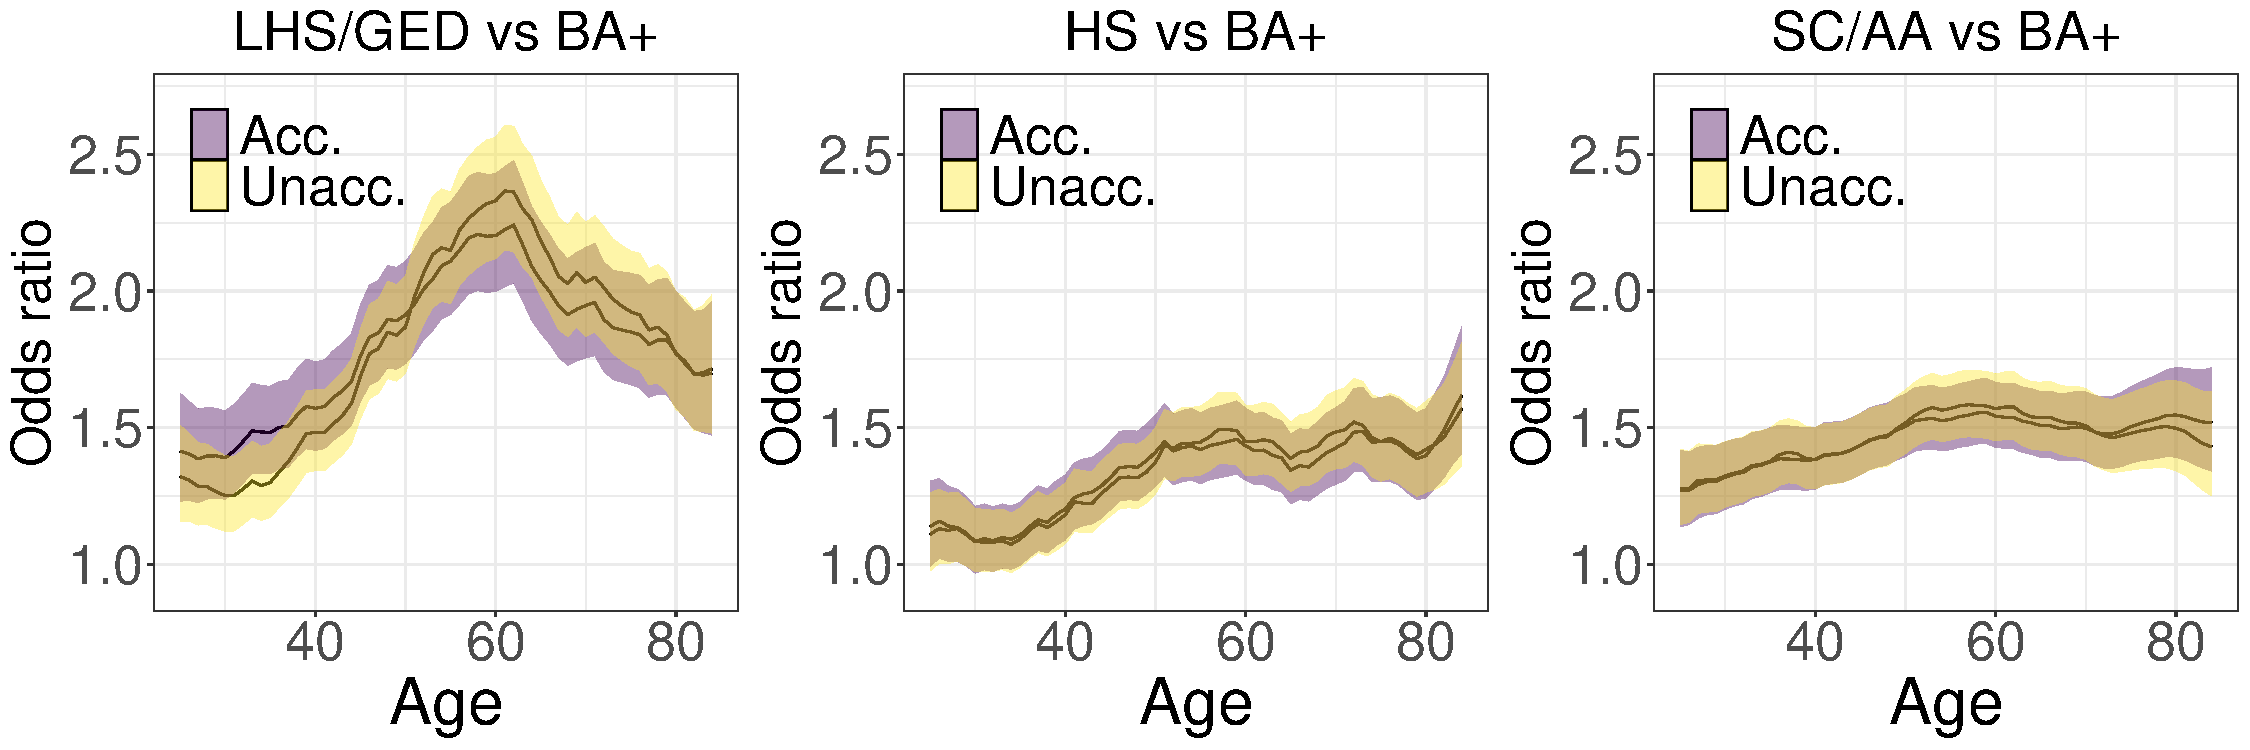
\includegraphics[width=\textwidth]{Figures/lincomb_hajek_f_age.pdf}
    \end{subfigure}
    \vskip\baselineskip\vspace{-0.3cm}
    \begin{subfigure}[t]{\textwidth}   
        \centering 
        \caption[]%
        {}    
        \label{figure:Application2:cohort_diff_f}
        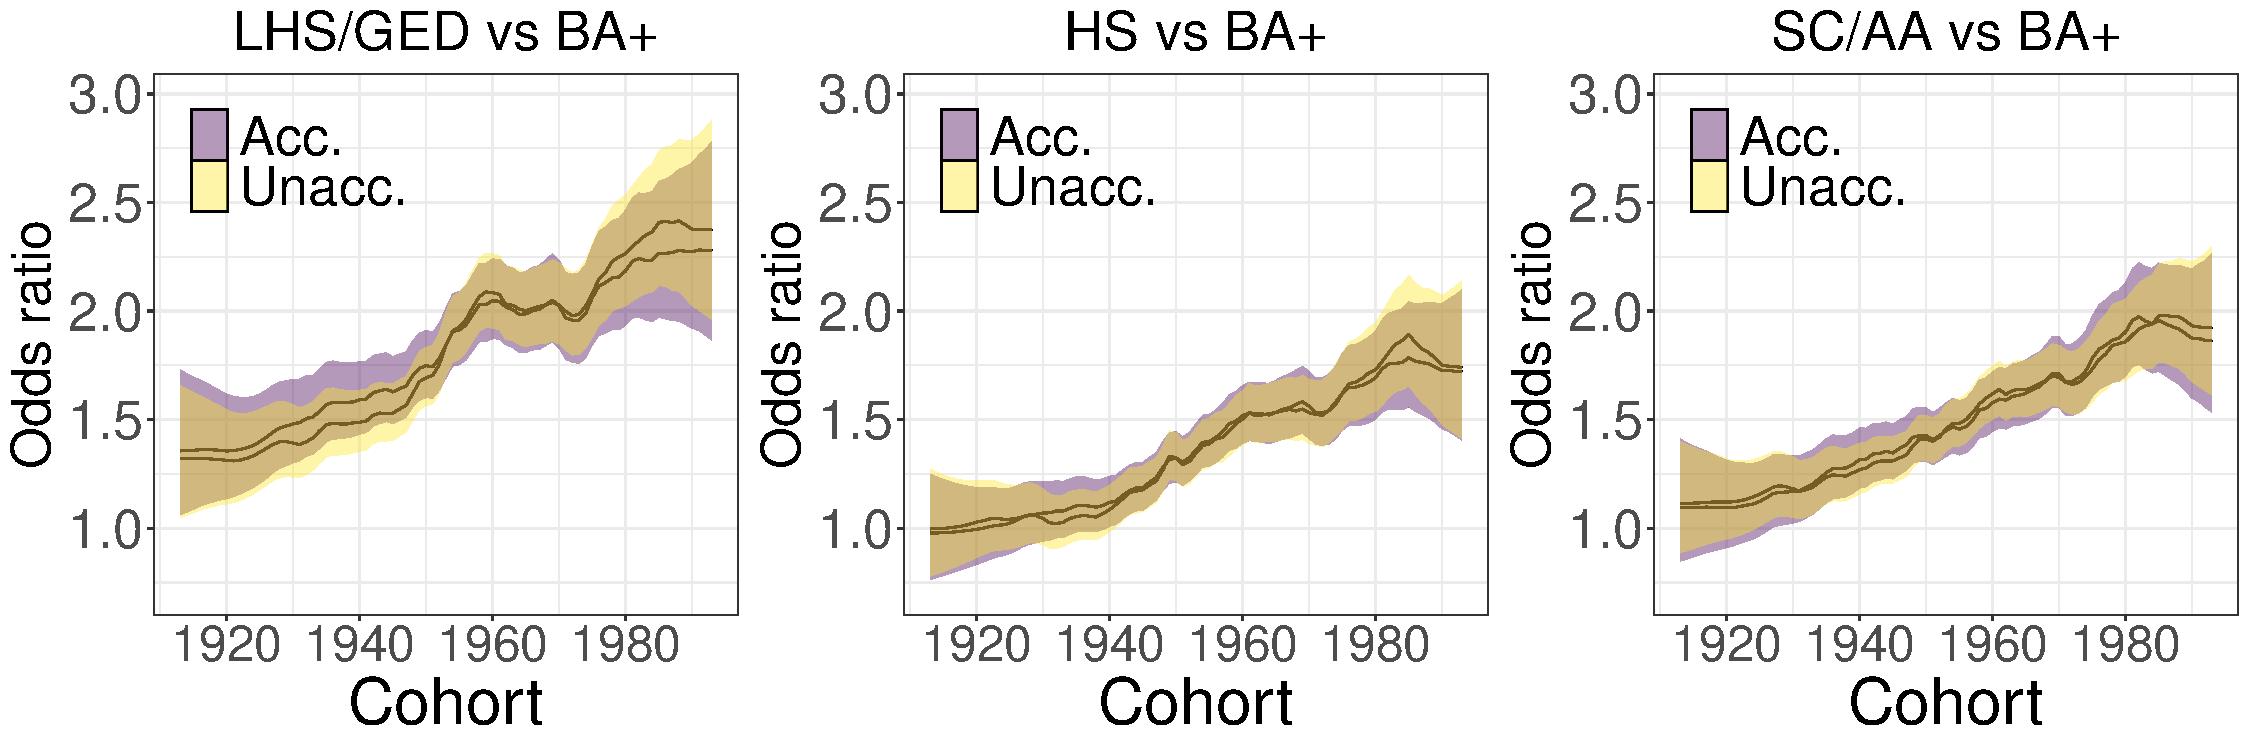
\includegraphics[width=\textwidth]{Figures/lincomb_hajek_f_cohort.pdf}
    \end{subfigure}
    \vspace{-0.2cm}
    \caption{Posterior median odds ratios together with $95\%$ credible intervals for less than high school (LHS), high school (HS), and some college/associate of arts degree (SC/AA) levels of attained education with respect to bachelor or higher education (BA+), over \textbf{(a)} age and \textbf{(b)} cohorts. The trends are shown for females using the aPc model accounting for the survey design, and are compared to the unaccounted estimates.}
    \label{figure:Application2:lincombs_f}
\end{figure}

%Best model males
\begin{figure}[h!]
    \centering
    \begin{subfigure}[b]{\textwidth}   
        \centering 
        \caption[]%
        {}    
        \label{figure:Application2:age_diff_m}
        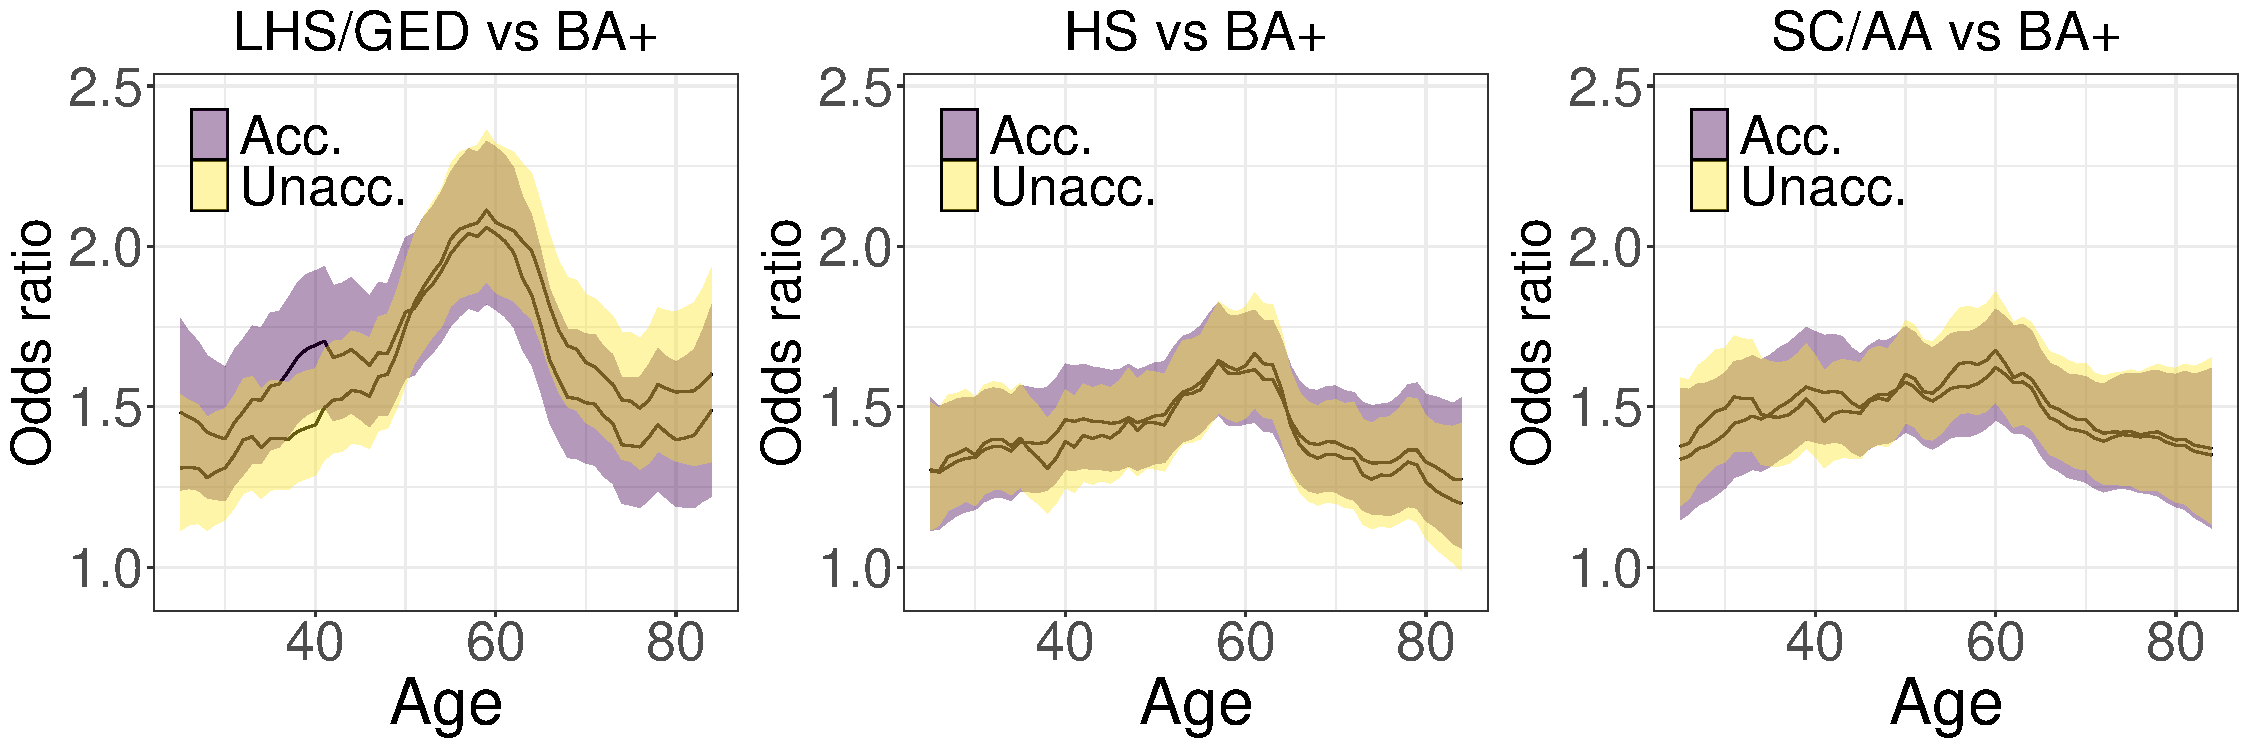
\includegraphics[width=\textwidth]{Figures/lincomb_hajek_m_age.pdf}
    \end{subfigure}
    \vskip\baselineskip\vspace{-0.3cm}
    \begin{subfigure}[b]{\textwidth}   
        \centering 
        \caption[]%
        {}    
        \label{figure:Application2:cohort_diff_m}
        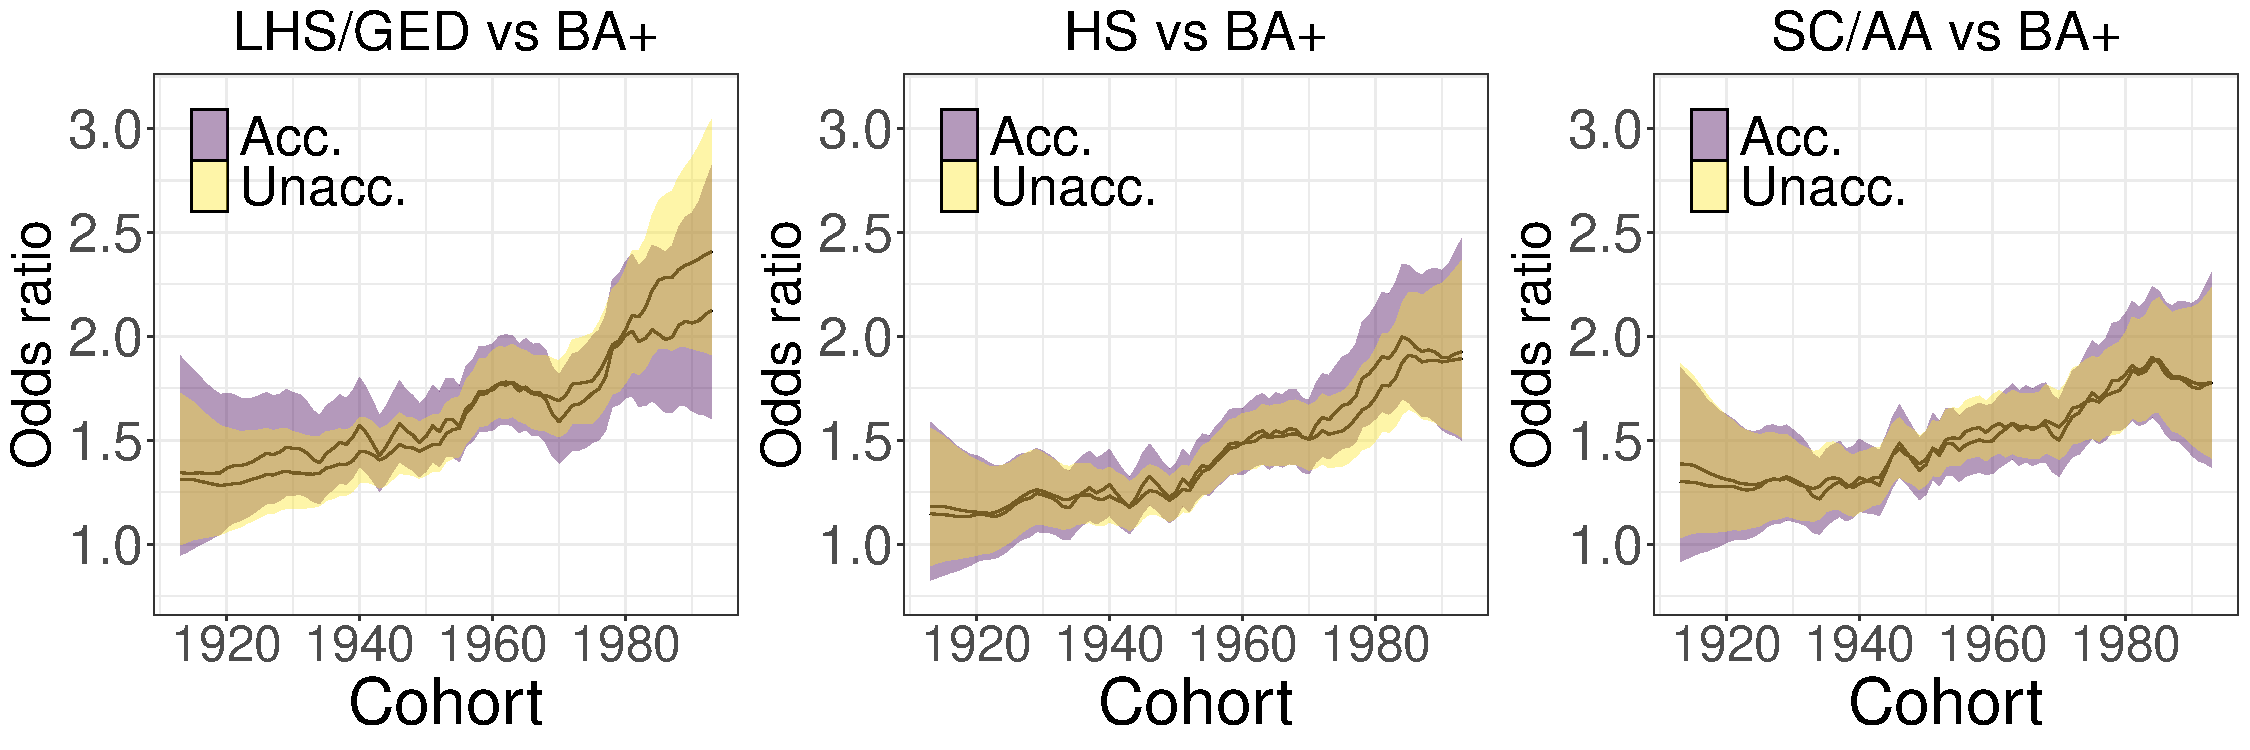
\includegraphics[width=\textwidth]{Figures/lincomb_hajek_m_cohort.pdf}
    \end{subfigure}
    \vspace{-0.2cm}
    \caption{Posterior median odds ratios together with $95\%$ credible intervals for less than high school (LHS), high school (HS), and some college/associate of arts degree (SC/AA) levels of attained education with respect to bachelor or higher education (BA+), over \textbf{(a)} age and \textbf{(b)} cohorts. The trends are shown for males using the aPc model accounting for the survey design, and are compared to the unaccounted estimates.}
    \label{figure:Application2:lincombs_m}
\end{figure}

%Over cohorts
\subsubsubsection*{Trends over cohorts}
\vspace{-0.2cm}
For the estimated odds ratios over cohorts in female and male data, seen in Figures \ref{figure:Application2:cohort_diff_f} and \ref{figure:Application2:cohort_diff_m}, the models accounting to the survey design appear to make similar estimates to the unaccounting models for all levels of attained education. Some different estimates are visible, though the differences are usually minor in the range between $0$ and $0.1$. That is, accounting for the complex sampling design does not change the overall pattern of the findings. There are, however, some differences, most notably for LHS/GED level of attained education compared to BA+ level in the most recent birth cohorts. Consequently, we again observe no overall change in the trends. In this region, notice that the credible intervals are very wide, meaning that there is higher uncertainty in the estimates. 

%Multiple models results
\subsubsubsection*{Trends in alternative models}
\vspace{-0.2cm}
The posterior medians of the odds ratio in the top four models chosen by model selection in Section \ref{section:application2:model_selection}, along with $95\%$ credible intervals are shown in Figure \ref{figure:Application2:lincombs_f_survey} for female data, and Figure \ref{figure:Application2:lincombs_m_survey} for male data. Figures \ref{figure:Application2:age_diff_f_survey} and \ref{figure:Application2:age_diff_m_survey} show the odds ratios over age in the aPc, apC, and aPC models. As observed in the same set of models when not accounting for the survey design, in Section \ref{section:application1:results}, the trends in odds ratio are very similar for the apC and aPC models, but they were significantly different from trends in the aPc model. Compared to the trends in the unaccounting models in Figures \ref{figure:Application1:age_diff_f} and \ref{figure:Application1:age_diff_m}, we observe more similarity between the trends in the models accounting for the survey design. In the odds ratios over period, in Figures \ref{figure:Application2:age_diff_f_survey} and \ref{figure:Application2:age_diff_m_survey}, we again have only one model to consider, namely the apC model. We observe trends that are either flat and then rise from 2005, or are slightly increasing overall. Interestingly, the trends using male data fluctuate less in the accounting models compared to the unaccounting models in Figures \ref{figure:Application1:age_diff_f} and \ref{figure:Application1:age_diff_m}. Over cohorts, in Figures \ref{figure:Application2:cohort_diff_f_survey} and \ref{figure:Application2:cohort_diff_m_survey}, we observe that the estimated trends in the aPc and APc models. The observations made for the cohort trends in the accounting models are similar to the trends of their unaccounting counterparts. In female data in particular, we again observe the steep drop for LHS/GED level of attained education in the APc model between the $1960$ and $1970$ cohorts. This drop is also visible when using the male data, though again to a lesser extent. Overall, when accounting for the survey design, the differences between models of different configurations of shared and stratum-specific effects are similar to those observed when not accounting for the design, albeit the differences are somewhat smaller in the design accounting models.

%Top3 models female
\begin{figure}[h!]
    \centering
    \begin{subfigure}[b]{\textwidth}   
        \centering 
        \caption[]%
        {}    
        \label{figure:Application2:age_diff_f_survey}
        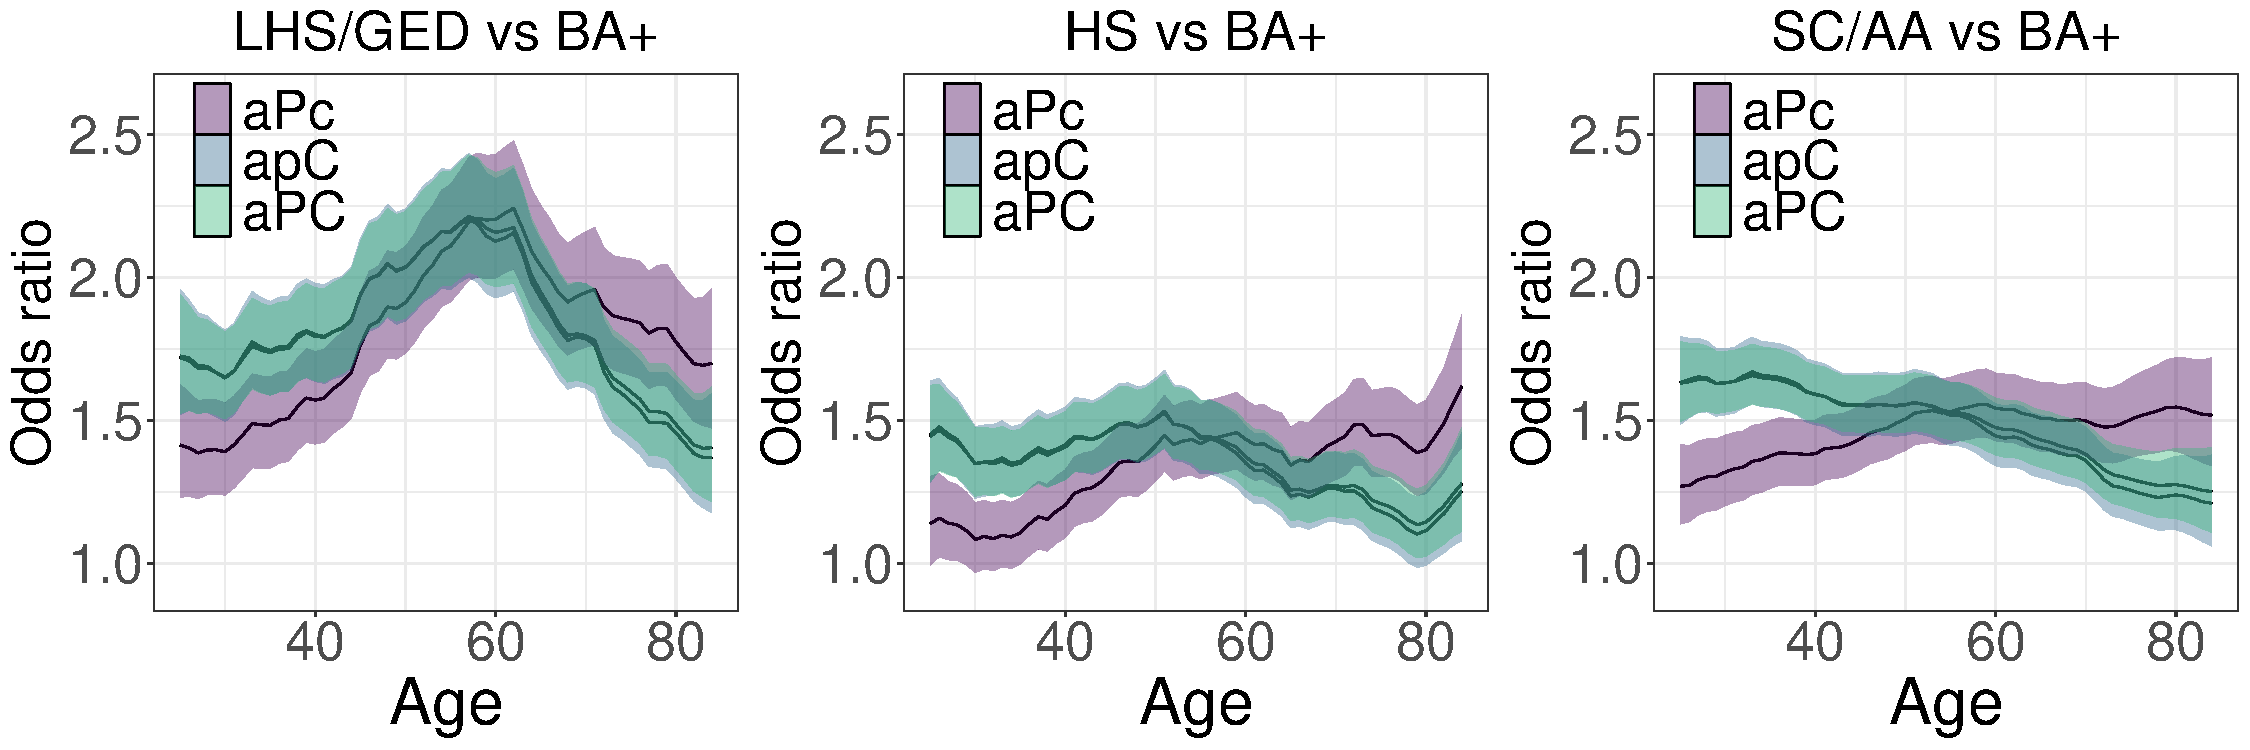
\includegraphics[width=\textwidth]{Figures/lincomb_age_f_survey.pdf}
    \end{subfigure}
    \vskip\baselineskip\vspace{-0.3cm}
    \begin{subfigure}[b]{\textwidth}   
        \centering 
        \caption[]%
        {}    
        \label{figure:Application2:period_diff_f_survey}
        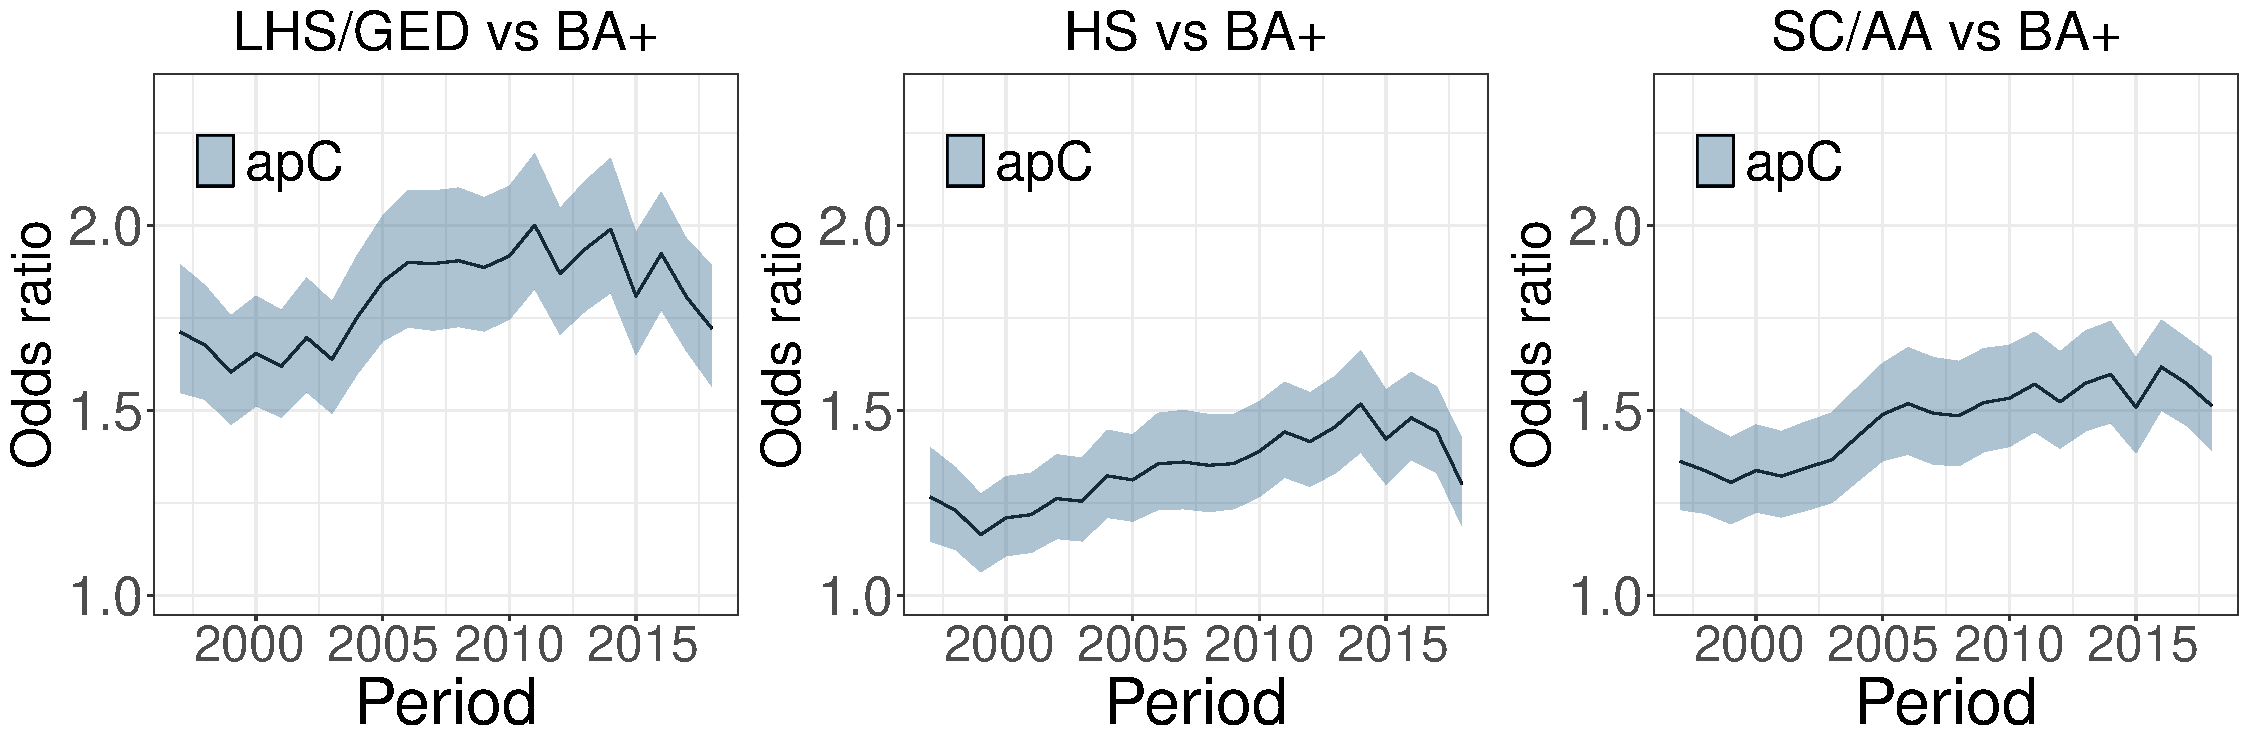
\includegraphics[width=\textwidth]{Figures/lincomb_period_f_survey.pdf}
    \end{subfigure}
    \vskip\baselineskip\vspace{-0.3cm}
    \begin{subfigure}[b]{\textwidth}   
        \centering 
        \caption[]%
        {}    
        \label{figure:Application2:cohort_diff_f_survey}
        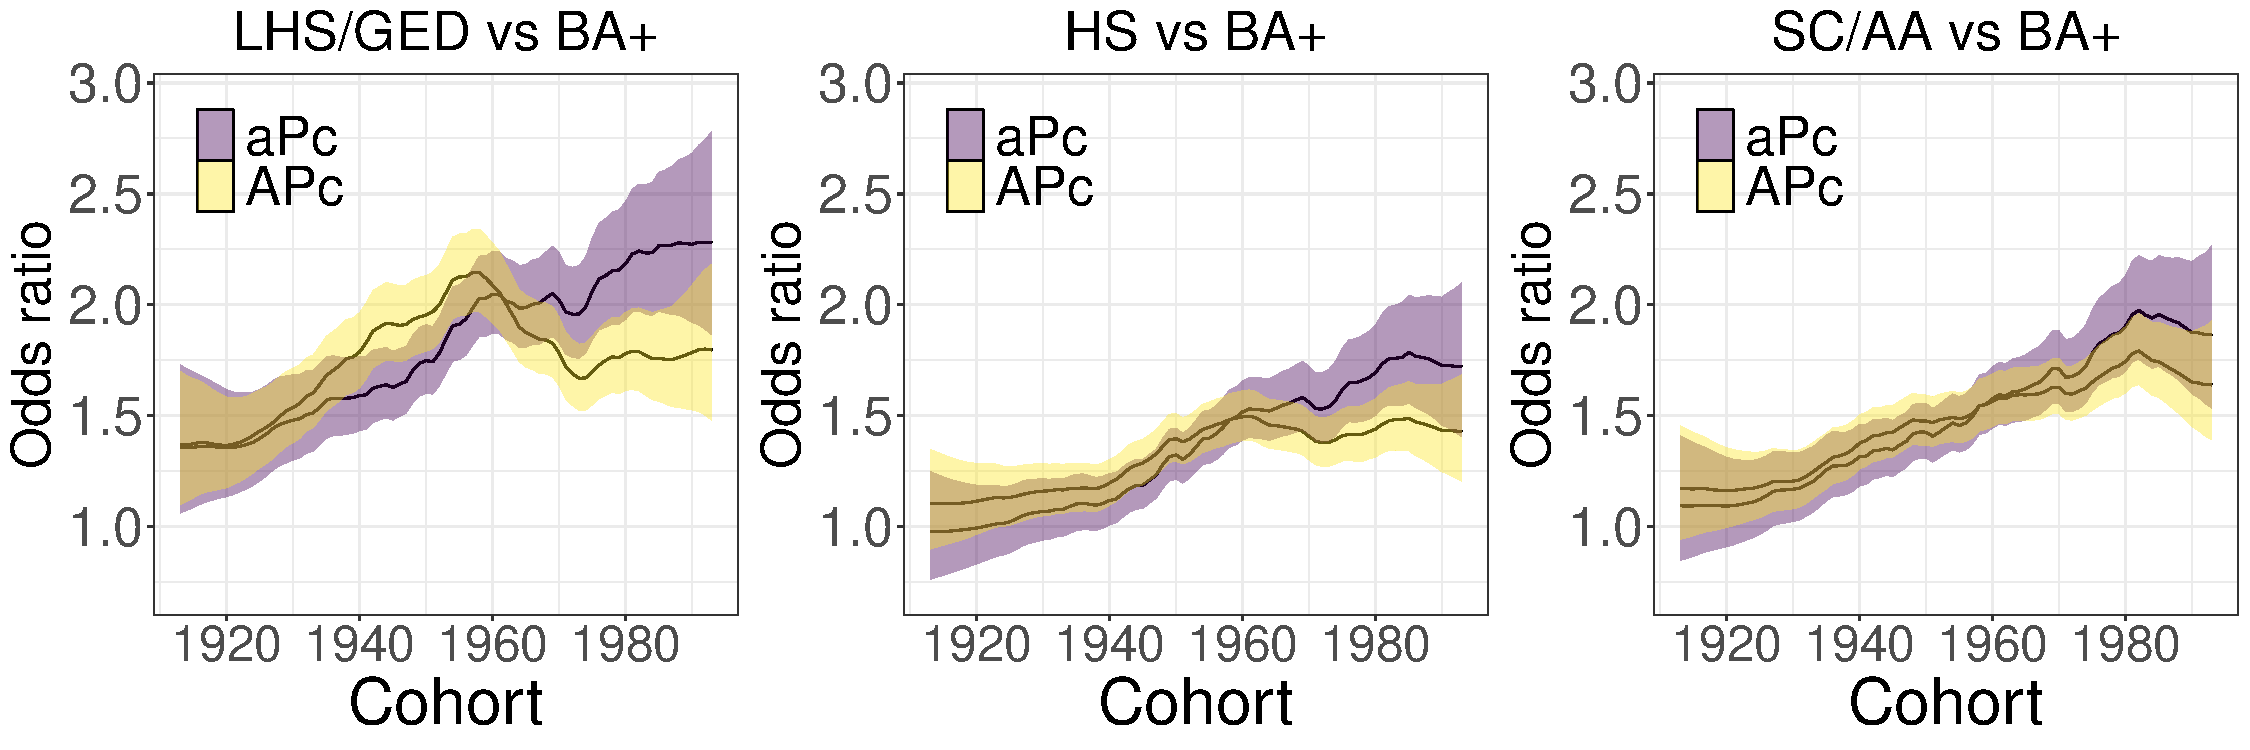
\includegraphics[width=\textwidth]{Figures/lincomb_cohort_f_survey.pdf}
    \end{subfigure}
    \vspace{-0.2cm}
    \caption{For females with less than high school (LHS), high school (HS), and some college/associate of arts degree (SC/AA) levels of attained education with respect to bachelor or higher education (BA+), the posterior median odds ratio in the top four models accounting for the survey design chosen by model selection over \textbf{(a)} age, \textbf{(b)} periods, and \textbf{(c)} cohorts, together with $95\%$ credible intervals.}
    \label{figure:Application2:lincombs_f_survey}
\end{figure}


%Top3 models male
\begin{figure}[h!]
    \centering
    \begin{subfigure}[b]{\textwidth}   
        \centering 
        \caption[]%
        {}    
        \label{figure:Application2:age_diff_m_survey}
        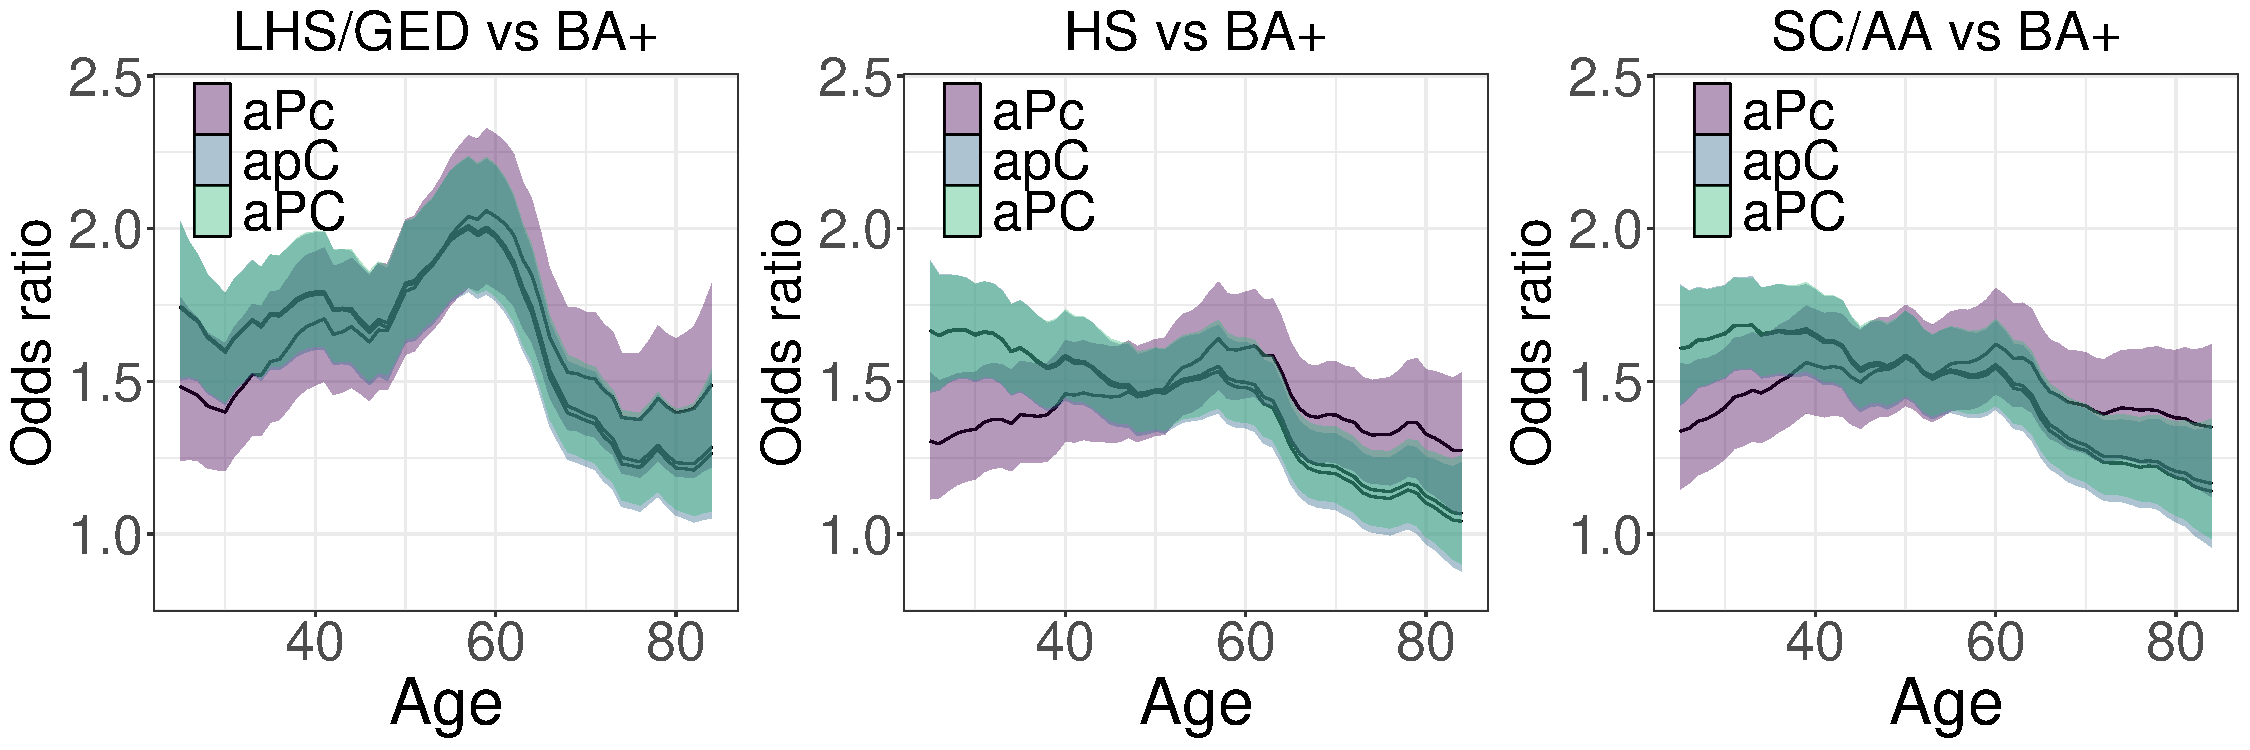
\includegraphics[width=\textwidth]{Figures/lincomb_age_m_survey.pdf}
    \end{subfigure}
    \vskip\baselineskip\vspace{-0.3cm}
    \begin{subfigure}[b]{\textwidth}   
        \centering 
        \caption[]%
        {}    
        \label{figure:Application2:period_diff_m_survey}
        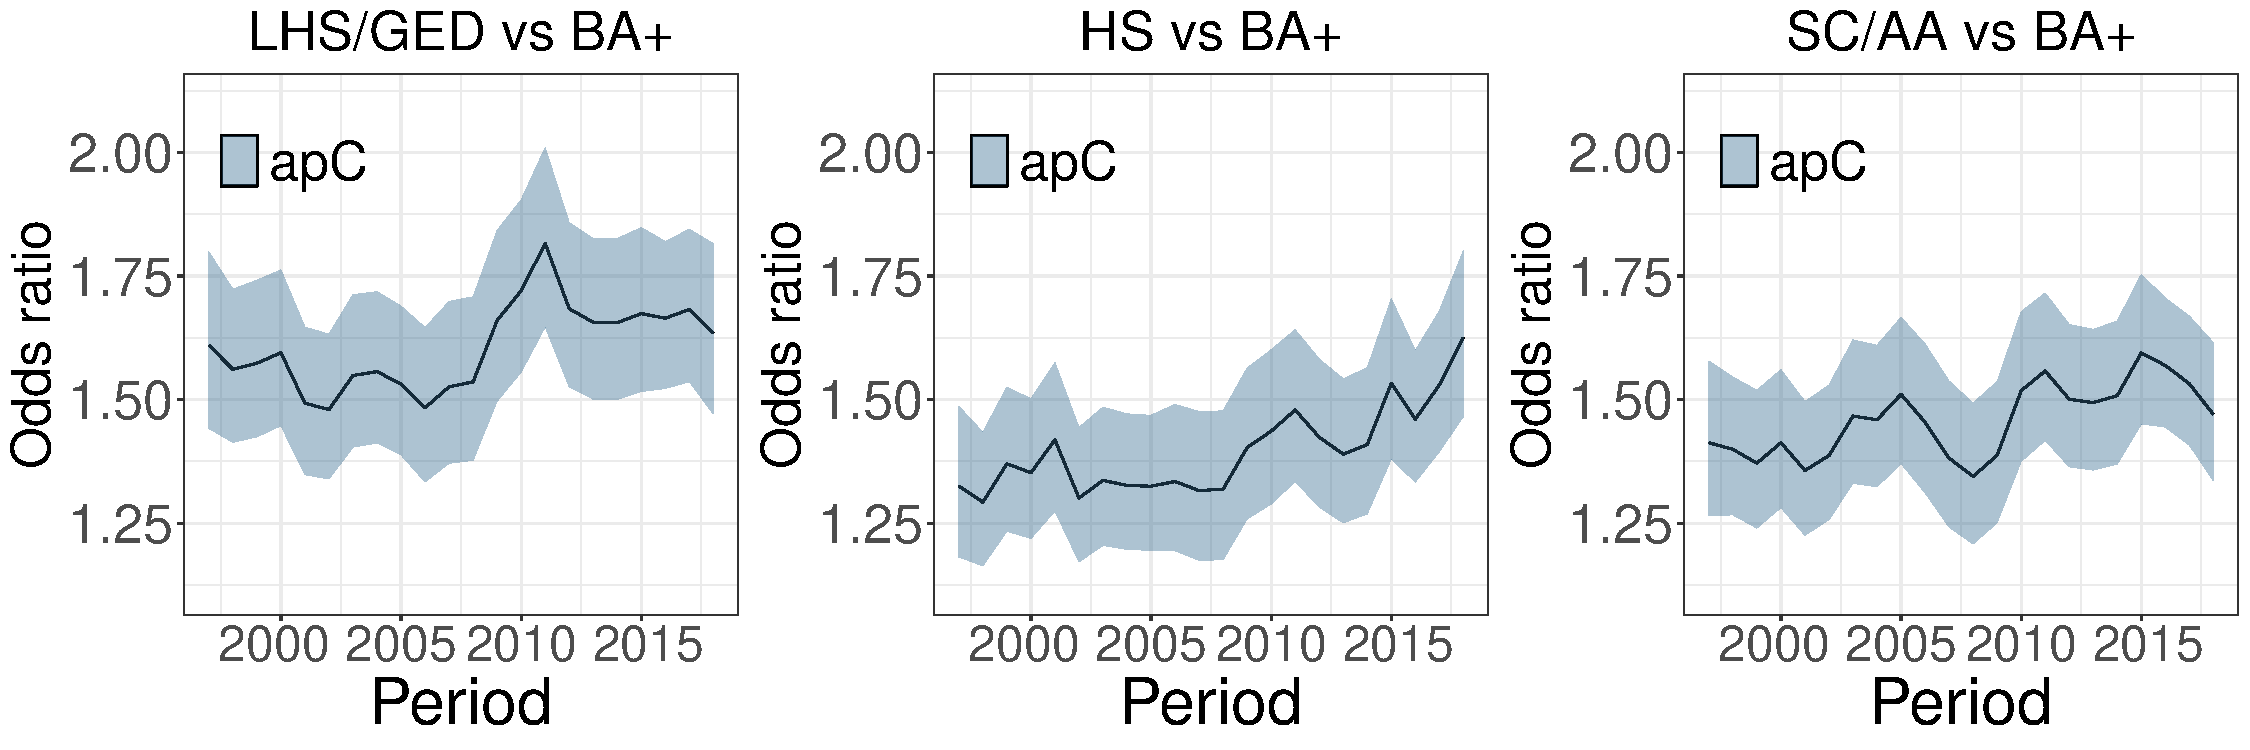
\includegraphics[width=\textwidth]{Figures/lincomb_period_m_survey.pdf}
    \end{subfigure}
    \vskip\baselineskip\vspace{-0.3cm}
    \begin{subfigure}[b]{\textwidth}   
        \centering 
        \caption[]%
        {}    
        \label{figure:Application2:cohort_diff_m_survey}
        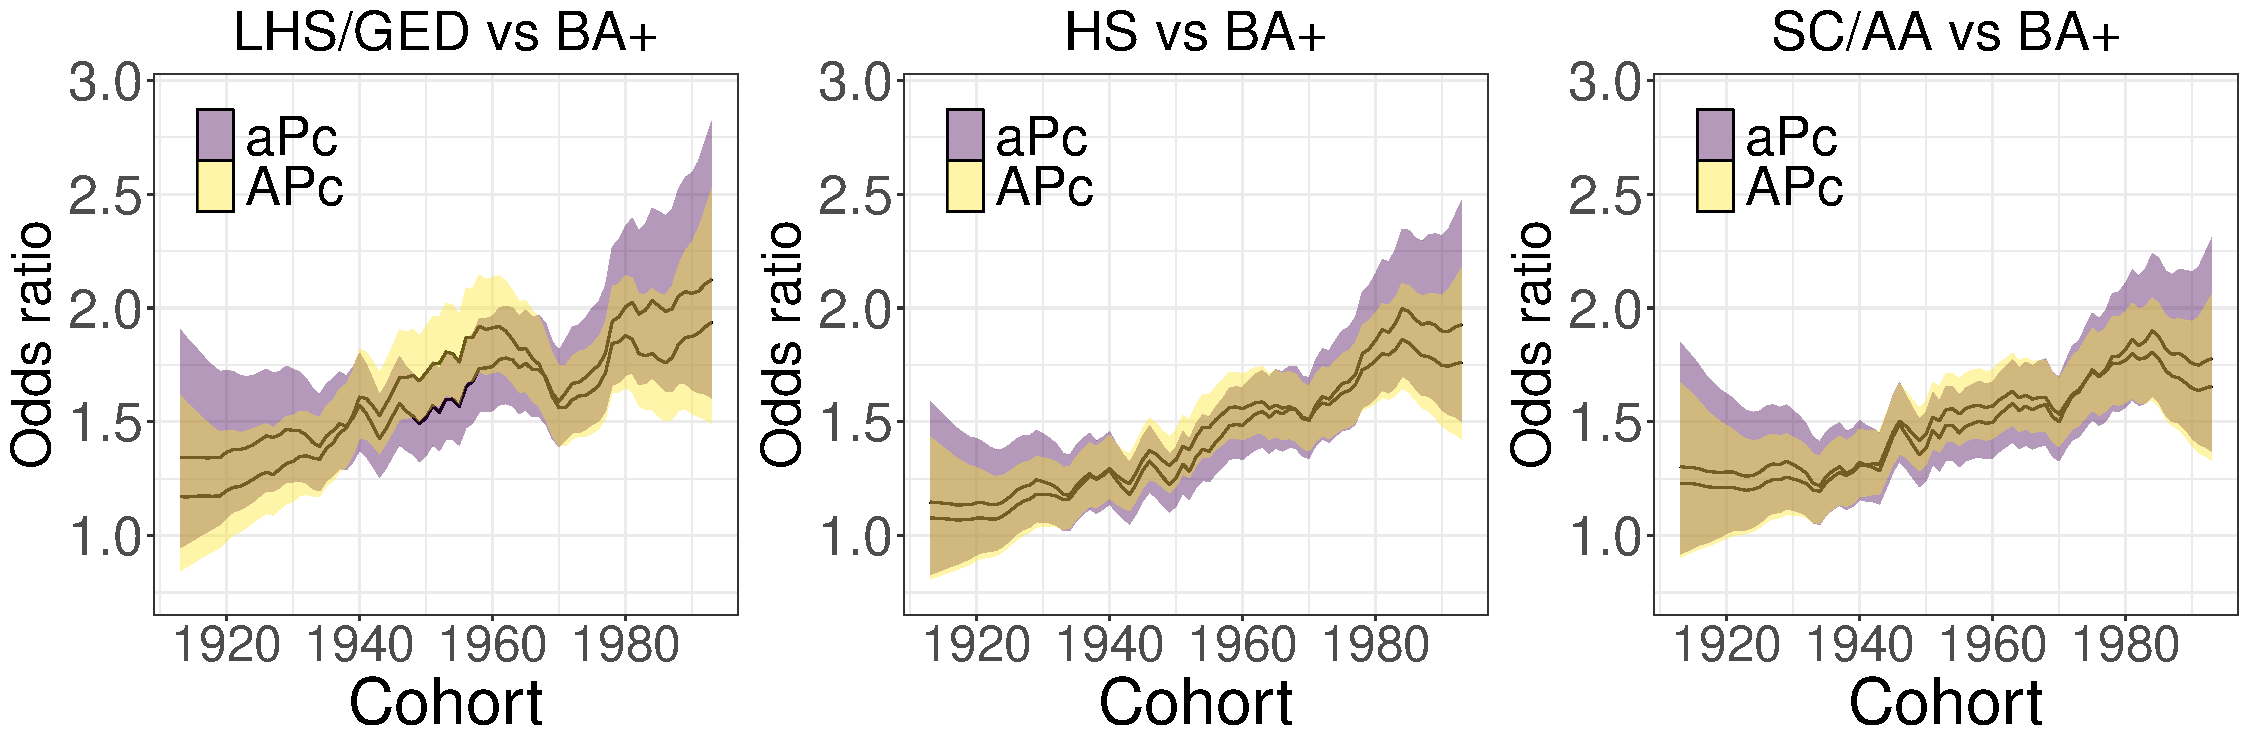
\includegraphics[width=\textwidth]{Figures/lincomb_cohort_m_survey.pdf}
    \end{subfigure}
    \vspace{-0.2cm}
    \caption{For males with less than high school (LHS), high school (HS), and some college/associate of arts degree (SC/AA) levels of attained education with respect to bachelor or higher education (BA+), the posterior median odds ratio in the top four models accounting for the survey design chosen by model selection over \textbf{(a)} age, \textbf{(b)} periods, and \textbf{(c)} cohorts, together with $95\%$ credible intervals.}
    \label{figure:Application2:lincombs_m_survey}
\end{figure}


\FloatBarrier
\subsection{Discussion}
\label{section:application2:discussion}
\subsubsubsection*{Summary}
\vspace{-0.2cm}
In this section, the survey design variables discussed in Section \ref{section:surveyData} were successfully incorporated in our Bayesian multivariate age-period-cohort model following the approach suggested by \cite{SurveyDesignMercer}. The survey design weights were included in the estimates using the Hájek estimator (Section \ref{section:application2:hajek}), while the PSU and STRATA design variables (Section \ref{section:surveyData}) were used to estimate the variance of the estimator. Computationally, the \texttt{survey} package was used to obtain the direct estimates with the corresponding variances. Model selection was carried out once more using logarithmic score, again selecting the aPc model with shared period effects, and stratum-specific age and cohort effects. Again, as discussed in Section \ref{section:APC-inference}, the estimated odds ratios are with respect to the highest level of education, BA+. 

%How compared to the regular results? Was the impact of survey designs great? Any further insights
\subsubsubsection*{Effects of accounting for the survey design}
\vspace{-0.2cm}
As we have seen from the estimated trends in the aPc model, the trends do not appear to change much when accounting for the survey design. Although the estimated odds ratios differ in certain regions, the overall shape, magnitudes, and interpretations of the trends remain largely the same in the accounting and unaccounting models. It is interesting to note that the width of the credible intervals appear to be roughly the same sizes in both the accounting and unaccounting models, meaning that aside from the different estimates caused by the survey weights, incorporating the survey design variables in the variance of the estimator did also not seem to affect the results much. Therefore, accounting for the survey design did not affect our conclusions to a great extent, but it does reassure us that our discussed points and interpretations on the unaccounting model in Section \ref{section:Application1:Dicussion} are still valid. While accounting for the survey design did not lead to different conclusions in this analysis, it cannot be said that this will be the case for all other analyses using APC models with different data. As we have demonstrated, accounting for the survey design weights in APC models is doable and does not require much extra effort. Therefore, it is recommended to incorporate these survey weights in future temporal analyses using APC models with survey data, to analyse the data properly.

%Variation in models
\subsubsubsection*{Trends in alternative models}
\vspace{-0.2cm}
Moreover, when accounting for the survey design, we saw that the estimated trends have become more similar between models with different combinations of shared and stratum-specific effects. Observing different trends when using different combinations of shared and stratum-specific effects is expected, since the underlying model assumptions are different. Over age, we still observe the inverse V-shaped trend for LHS/GED level of attained education, and over cohorts, we observe rising risk with more recent cohorts. An interesting twist lies in the trends over age for HS and SC/AA levels of attained education, where the alternative models without a stratum-specific cohort effect showed decreasing, rather than increasing trends. If we assume that the cohort effects are the same in all levels of attained education, we would then we observe that as participants with HS and SC/AA levels of attained education grow older, the risk of backpain compared to BA+ level is smaller. Thus, in these alternative models, the impact of education is considerably stronger in younger adults, and begins to even out to the levels observed for the BA+ level of attained education.

%Weirdness of GED still
\subsubsubsection*{Disparities in the LHS/GED educational group}
\vspace{-0.2cm}
In our comparison of the temporal trends between the accounting and unaccounting models, it was observed that the odds ratios differed the most for LHS/GED level of attained education. As has already been argued, the LHS/GED level of attained education stands out from the other levels of attained education by several measures. For this level, we have seen greater disparities in health and smaller sample sizes. Moreover, external socioeconomic factors for this level of education can be argued to have changed the most over the cohorts \citep{dowd2014life,montez2011trends,hendi2015trends}. Although accounting for the survey design did not provide much more insight into the trends of this level of attained education, the survey variables we incorporated still allow us to make better use of samples from subpopulations. Consequently, we will be continuing our analysis accounting for the survey design by considering only parts of the population.

\FloatBarrier
\subsection{Further investigation on a subpopulation}
\label{section:application2:extension}
Following our discussion of the observed trends in the aPc model when accounting for the survey design, in Section \ref{section:application2:discussion}, further investigation of the temporal trends is motivated, particularly for LHS/GED level of attained education. After consultation with the sociologist who provided us with the expert knowledge in Section \ref{section:application1:prior}, it was recommended to run the same analysis while accounting for the survey design using only white, U.S.-born participants. Other than education, critical driving factors of health include race/ethnicity and nativity. The composition of the LHS/GED educational group has changed dramatically over the years by several measures. One such measure is immigration, where many adult immigrants arrive with education corresponding to LHS/GED level. Consequently, for many of the years in their lives, they have been exposed to conditions and factors foreign to the U.S., in turn making the composition of the LHS/GED educational group more complex. Therefore, it would be interesting to see what happens to the temporal trends when we account for some effects of immigration. Since additional controls cannot be included at the moment, filtering the acquired NHIS survey data for only white, U.S-born participants may help mitigate potential confounding due to the changing composition of the educational groups. To this end, the same procedures to account for the survey design, as in Section \ref{section:application2:implementation}, are used on the subset of the data that includes only white, U.S.-born participants. Ideally, this would be compared against the complementary filtering, though this would create problems with data sparsity, since not every combination of age, period, cohort, and education would be represented in the data. Moreover, in this data, some triplets of age, period, and educational attainment level had no observations of back pain, and were remedied by fixing the observation to $0.01$ with an estimated variance of $1$, as before. This time, there were also some triplets in which all participants had back pain, and so this was remedied by fixing the observation to $0.99$, along with the estimated variance to $1$. The resulting temporal trends will be compared to those achieved using data on all participants, as presented in Section \ref{section:application2:results}. 

\subsubsection{Results}
\label{section:application2:extension:results}
\subsubsubsection*{Summary}
\vspace{-0.2cm}
By using the NHIS survey data on only white, U.S.-born participants, Figures \ref{figure:Application2:lincombs_f_filtered} and \ref{figure:Application2:lincombs_m_filtered} show the posterior median odds ratios in the aPc model when accounting for the survey design, along with $95\%$ credible intervals for females and males, respectively. The odds ratios are shown over age and cohorts in the respective subfigures, along with the corresponding estimates in the aPc model accounting for the survey design using survey data on all participants (as presented in Section \ref{section:application2:results}). For convenience, models using survey data on only white, U.S.-born participants are referred to as filtered models, while models using survey data on all participants is referred to as unfiltered models. As discussed in Section \ref{section:APC-inference}, all estimated odds ratios are with respect to the highest level of attained education, BA+. 

%Over age
\subsubsubsection*{Trends over age}
\vspace{-0.2cm}
Over age, in Figures \ref{figure:Application2:age_diff_f_filtered} and \ref{figure:Application2:age_diff_m_filtered}, we observe similar estimates of the odds ratios for HS and SC/AA levels of attained education. In females with these levels of attained education, the main differences between the filtered and unfiltered models are observed between age groups $25$ and $50$, with greater differences in males than females. Overall, the shape of the trends are similar, and the credible intervals overlap continuously, yielding no different interpretations. On the other hand, for LHS/GED level of attained education, noticeable differences in the estimated odds ratios are observed. In females, a nearly constant difference in odds ratio is observed between the filtered and unfiltered models, with the estimated median odds ratios being mostly outside the credible intervals of each other. The differences in odds ratio varies between $0.25$ and $0.4$, taking higher values in age groups younger than $60$. In females, this nearly constant difference is also observed, though also amplified to range between $0.25$ to $0.5$, again with larger differences in age groups younger than $60$. Consequently, we observe a much higher risk of back pain in the white, U.S-born population with LHS/GED level of attained education compared to the corresponding age groups with BA+ level of attained education. It is also worth noting that the credible intervals of odds ratios in the filtered models are much wider than their unfiltered counterpart only for LHS/GED level of attained education. 

%Over cohorts
\subsubsubsection*{Trends over cohorts}
\vspace{-0.2cm}
Over cohorts, as shown in Figures \ref{figure:Application2:cohort_diff_f_survey} and \ref{figure:Application2:cohort_diff_m_survey} for males and females, respectively, we again observe similarities between the filtered and unfiltered models for HS and SC/AA levels of attained education, and dissimilarities for LHS/GED level of attained education. For HS and SC/AA levels of attained education, the differences in odds ratios over cohorts compared to the differences over age is smaller, though there are some differences in the estimates of the most recent cohorts. Overall, these differences do not change the overall shape and interpretations of the trends. We observe major differences for LHS/GED level of attained education, though over cohorts these differences are expressed differently for each sex. For females in older cohorts, the differences in the estimated odds ratios are around $0.25$, increasing gradually to nearly $1.2$ by the most recent cohorts. At most, this yields an estimated odds ratio of $3.5$ for the most recent cohorts, and a minimum of $1.5$ for the oldest cohorts. In males, we observe similar estimates between the filtered and unfiltered models from the $1913$ to $1940$ birth cohorts, after which the odds ratios in the filtered models rapidly increases to $2.5$ by the $1960$ birth cohort, at which point the unfiltered model estimates odds ratios around $1.75$. Between the $1960$ and $1993$ birth cohorts, the estimates of the filtered model fluctuates a lot, though it decreases to estimates comparable to that of the unfiltered model by the $1993$ birth cohort. The credible intervals are again observed to be significantly wider in the filtered model than the unfiltered model for LHS/GED level of attained education. 

\begin{figure}[h!]
    \centering
    \begin{subfigure}[b]{\textwidth}   
        \centering 
        \caption[]%
        {}    
        \label{figure:Application2:age_diff_f_filtered}
        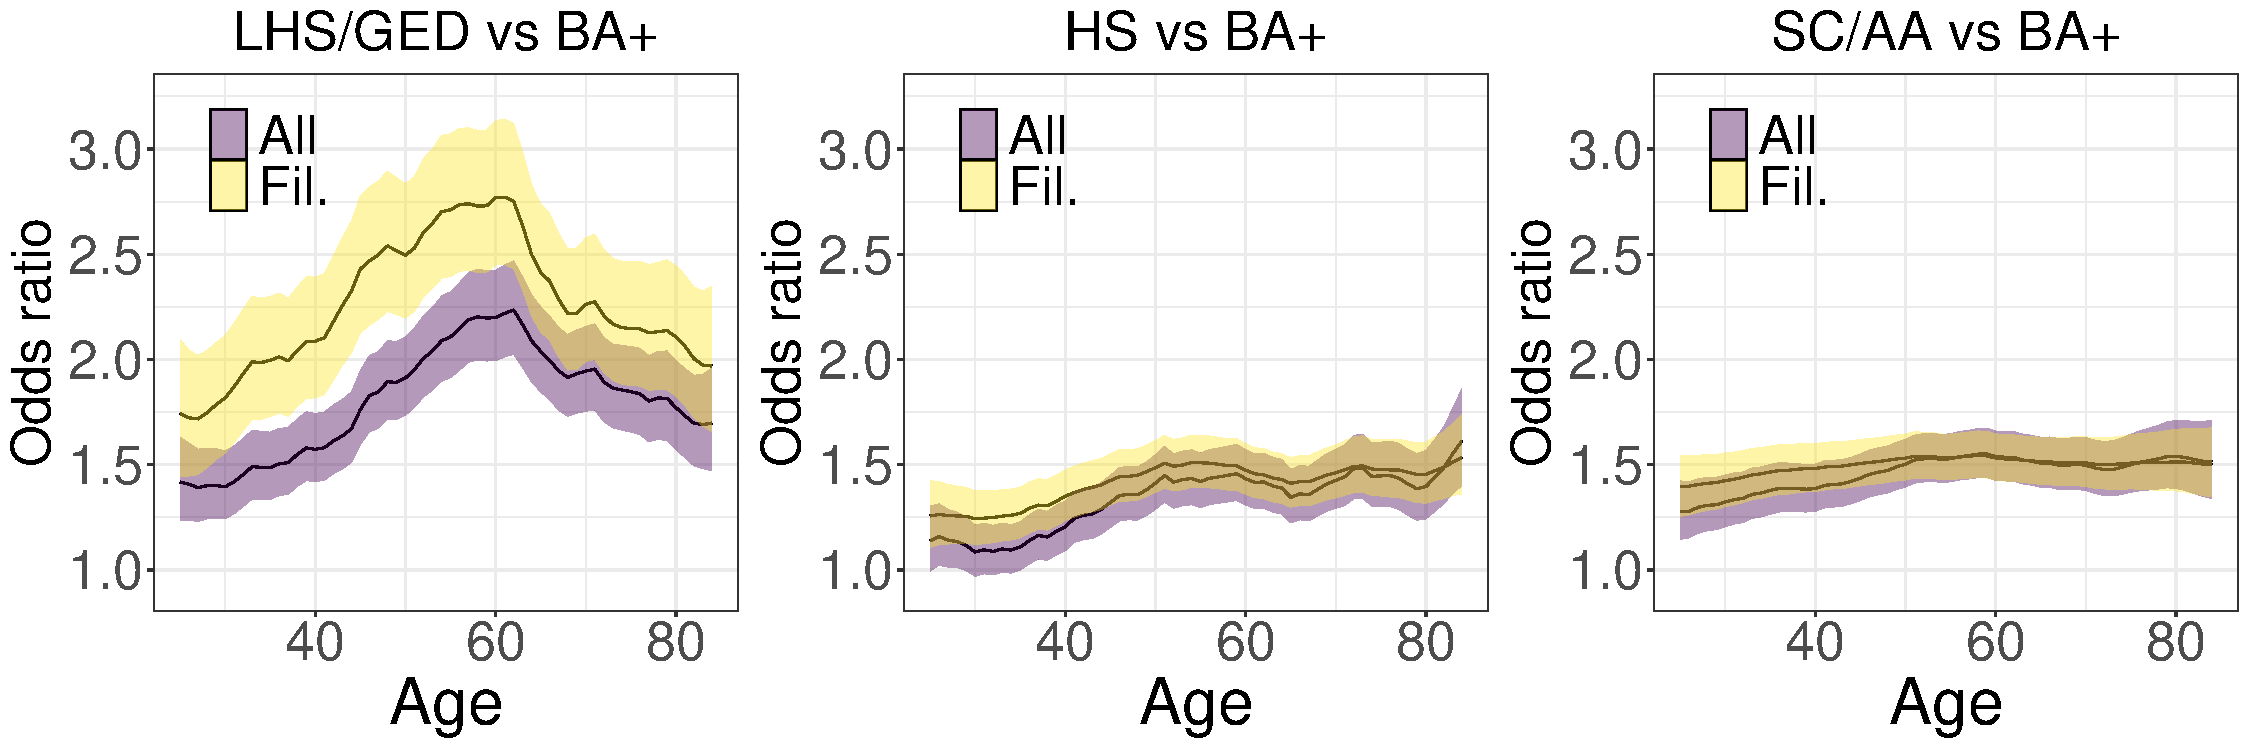
\includegraphics[width=\textwidth]{Figures/lincomb_survey_filtered_age_f.pdf}
    \end{subfigure}
    \vskip\baselineskip\vspace{-0.3cm}
    \begin{subfigure}[b]{\textwidth}   
        \centering 
        \caption[]%
        {}    
        \label{figure:Application2:cohort_diff_f_filtered}
        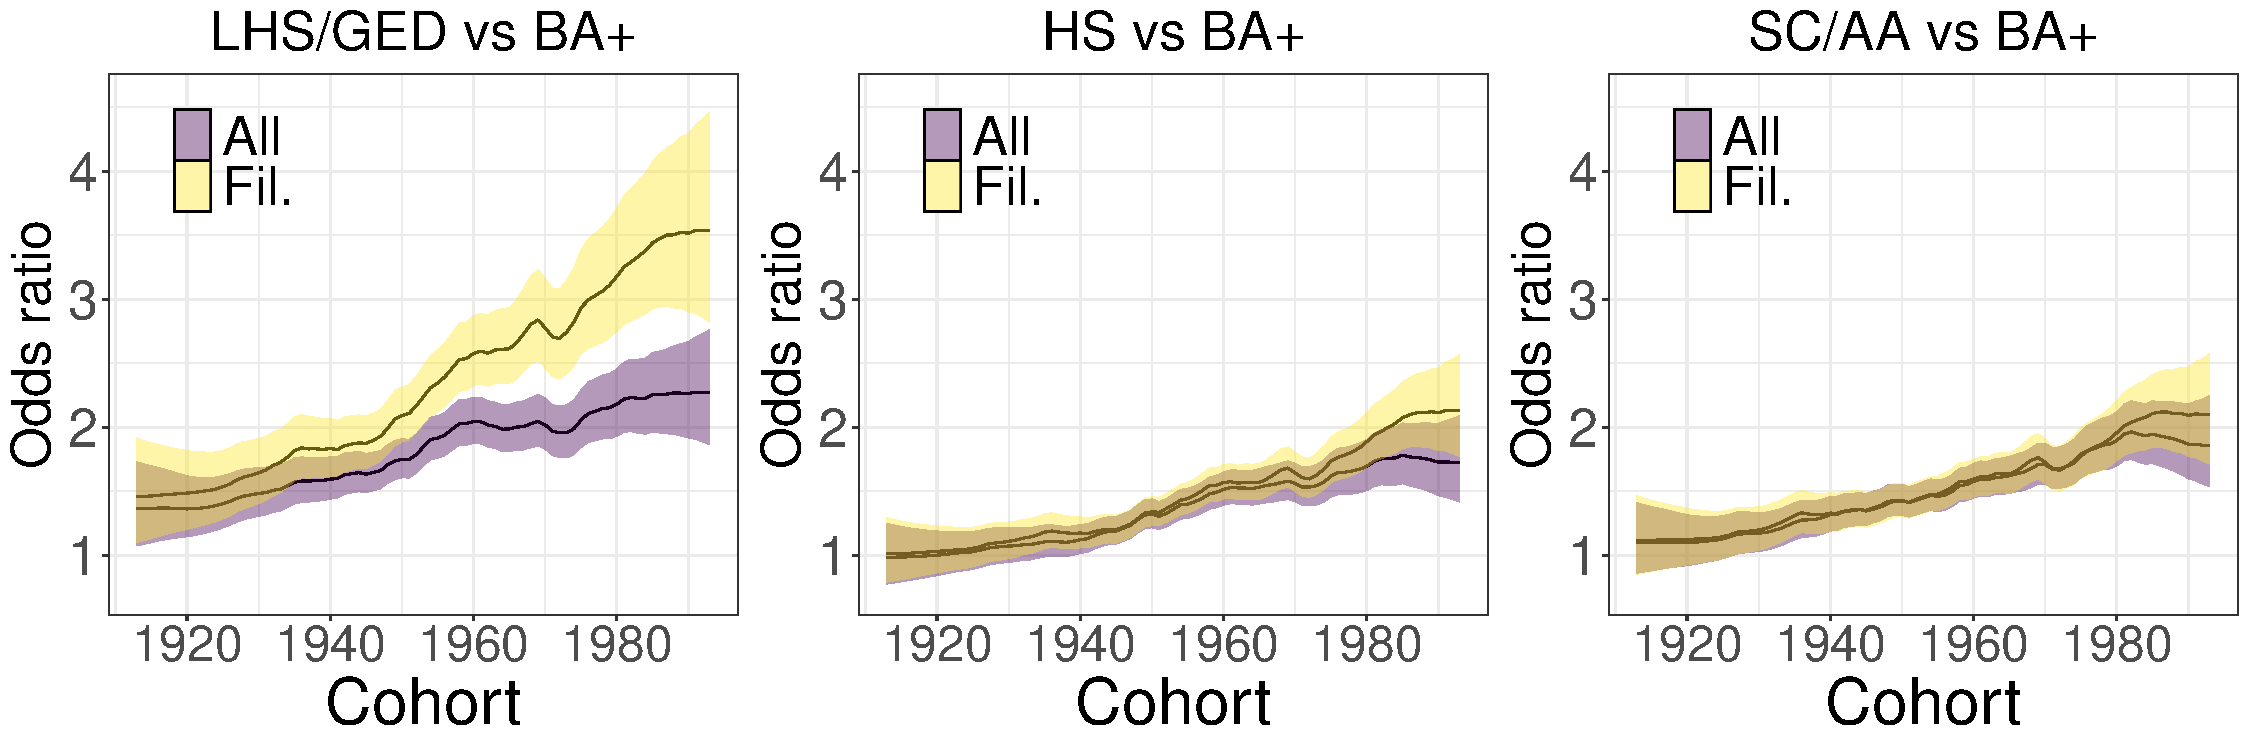
\includegraphics[width=\textwidth]{Figures/lincomb_survey_filtered_cohort_f.pdf}
    \end{subfigure}
    \vspace{-0.2cm}
    \caption{For less than high school (LHS), high school (HS), and some college/associate of arts degree (SC/AA) levels of attained education with respect to bachelor or higher education (BA+) level, the posterior median odds ratio over \textbf{(a)} age and \textbf{(b)} cohorts, in the aPc model accounting for the survey design along with $95\%$ credible intervals. The trends are shown using all female data (All) and using data on only white, U.S.-born females (Fil.).}
    \label{figure:Application2:lincombs_f_filtered}
\end{figure}

\begin{figure}[h!]
    \centering
    \begin{subfigure}[b]{\textwidth}   
        \centering 
        \caption[]%
        {}    
        \label{figure:Application2:age_diff_m_filtered}
        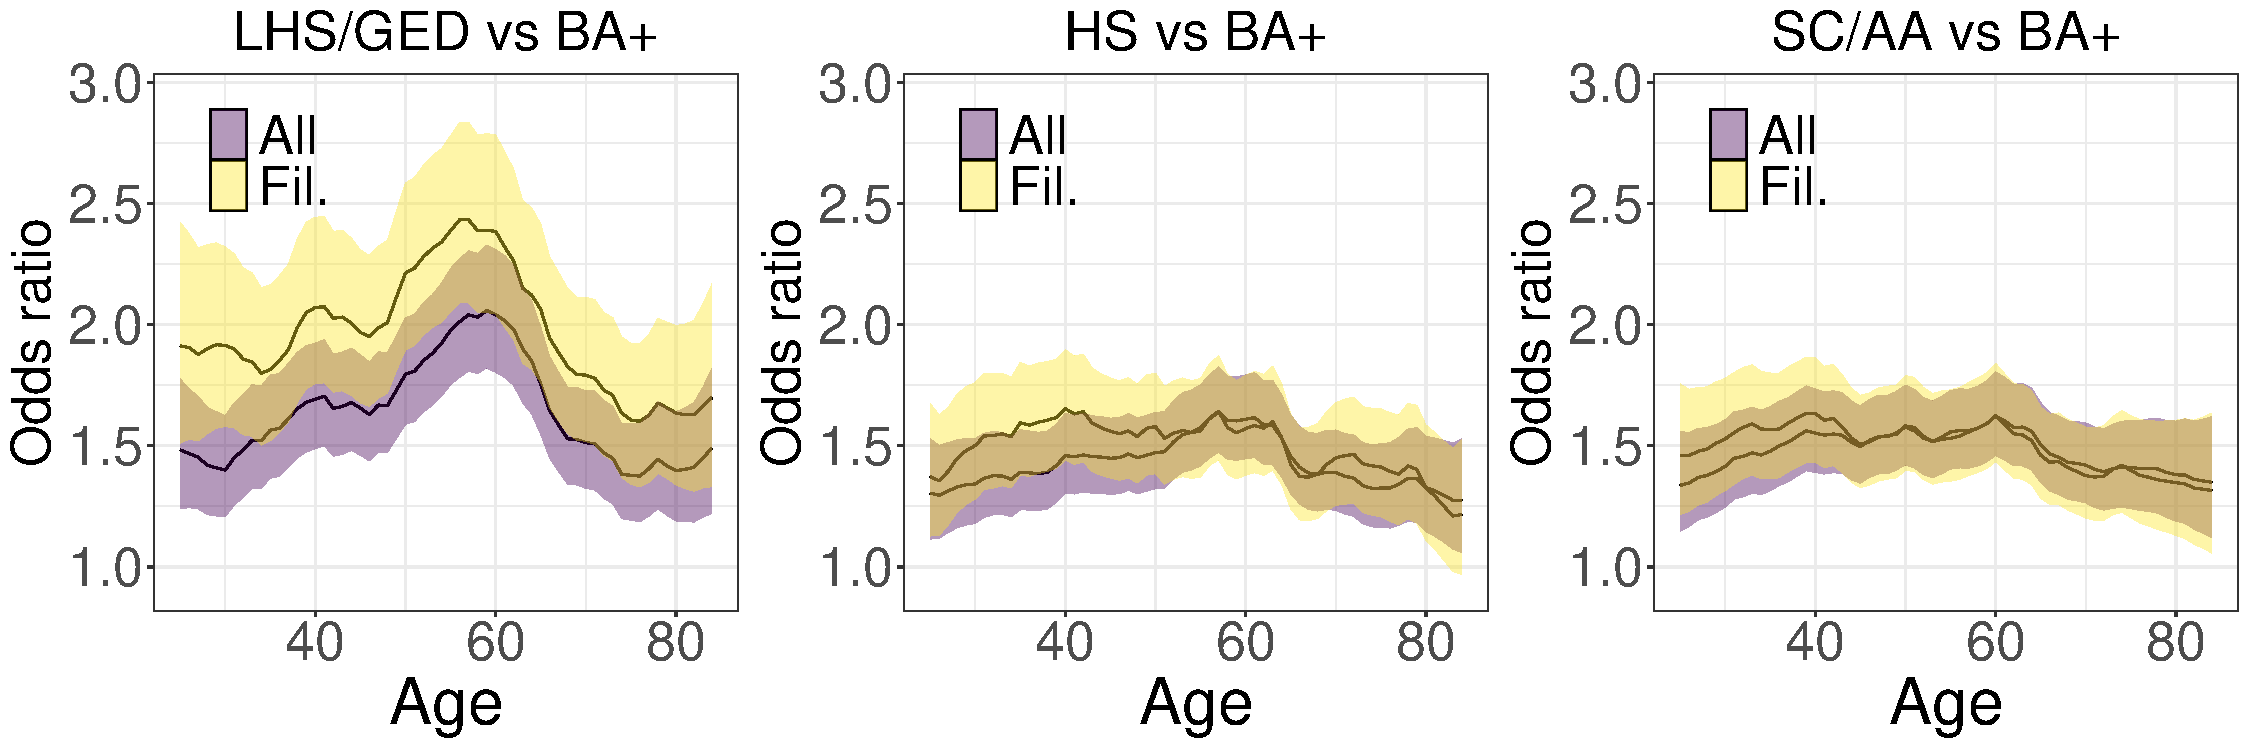
\includegraphics[width=\textwidth]{Figures/lincomb_survey_filtered_age_m.pdf}
    \end{subfigure}
    \vskip\baselineskip\vspace{-0.3cm}
    \begin{subfigure}[b]{\textwidth}   
        \centering 
        \caption[]%
        {}    
        \label{figure:Application2:cohort_diff_m_filtered}
        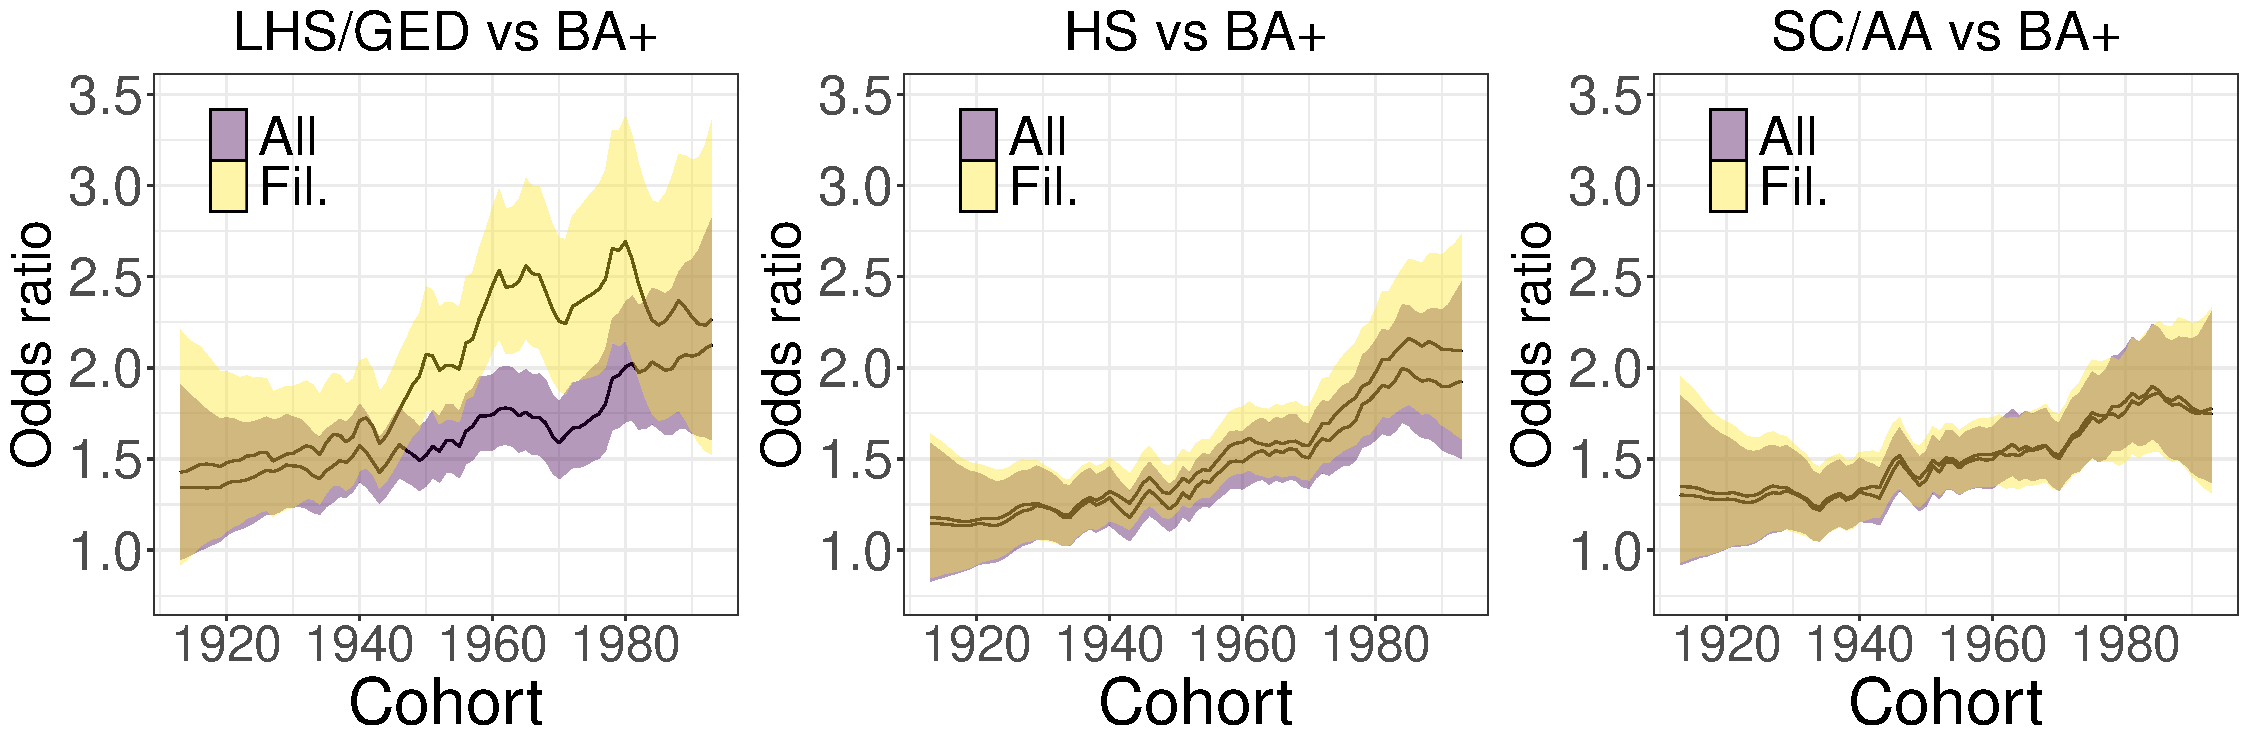
\includegraphics[width=\textwidth]{Figures/lincomb_survey_filtered_cohort_m.pdf}
    \end{subfigure}
    \vspace{-0.2cm}
    \caption{For less than high school (LHS), high school (HS), and some college/associate of arts degree (SC/AA) levels of attained education with respect to bachelor or higher education (BA+) level, the posterior median odds ratio over \textbf{(a)} age and \textbf{(b)} cohorts, in the aPc model accounting for the survey design along with $95\%$ credible intervals. The trends are shown using all male data (All) and using data on only white, U.S.-born males (Fil.).}
    \label{figure:Application2:lincombs_m_filtered}
\end{figure}

\subsubsubsection*{Additional smoothing}
\vspace{-0.2cm}
Using the filtered data, Figures \ref{figure:Application1:rw2_f_fil} and \ref{figure:Application1:rw2_m_fil} show the odds ratio trends over age and cohorts in the aPc model using RW1 and RW2 priors on the components of the latent field, for females and males respectively. As expected, the model using RW2 priors on the components of the latent field shows smoother temporal trends. The general shape of the trends are the same as when using RW1 priors, meaning that the introduction of more smoothing on the latent field did not drastically change the trends. 

\FloatBarrier
\subsubsection{Discussion}
\label{section:application2:extension:discussion}
In this short additional investigation, we attempted to eliminate the effects of some of the external factors that may have been present in particular for the LHS/GED educational group, by selecting only white, U.S.-born individuals for our analysis. Relying on the survey design adjustments, we saw that despite selecting only a subset of the total participants, we achieved estimates with similar uncertainty as in the model that uses all participants with HS and SC/AA levels of attained education. On the other hand, for LHS/GED level of attained education, large differences were observed between the models, with the filtered model displaying much larger credible intervals, resulting in more uncertainty in the estimated odds ratios. Despite the larger credible intervals, we identify regions in which the credible intervals of the models do not overlap, indicating that the differences are quite noticeable. 

In interpreting these results, it is important to keep in mind that in the filtered and unfiltered models, the educational group we compare against, BA+, is also affected by the filtering. That is, in the filtered model, we compared white, U.S.-born participants with LHS/GED level of attained education, to the white, U.S.-born participants with BA+ level of attained education. Though we expect the effects of immigration to be expressed the most for LHS/GED level of attained education, it may also affect the other levels of education as well. Should the white, U.S.-born only subset of the BA+ educational group be comparable to the BA+ educational group as a whole, one may then argue that our results show increased disparities in risk of back pain. If the white, U.S.-born subset of the BA+ educational group is different from the whole, then the observed differences could be due to the better health of this subpopulation. However, since we observed very similar trends for HS and SC/AA levels of attained education compared to BA+, it appears that the LHS/GED level of education is the odd one out once more. Consequently, our results indicate larger educational differences in the white, U.S.-born participants, though the aid of sociologists are again needed to further discuss potential causes of the observed differences. 















\FloatBarrier
\newpage

\section{Closing remarks}
\label{section:application2:conclusion}
In this thesis, I have investigated survey data on chronic back pain in United States adults aged 25 to 84 in the period 1997 to 2018, stratified into four educational groups. The goal was to investigate how disparities in back pain across educational groups has evolved using three time scales, namely with age, periods, and birth cohorts. To this end, I implemented a Bayesian multivariate age-period-cohort model using smoothing priors on the latent field. For model inference I used \texttt{INLA} in \texttt{R}. I achieved in smooth incorporation of provided sociological expert knowledge into the hyperpriors on the latent field using the HD and PC prior frameworks through \texttt{makemyprior}. Furthermore, I conducted model selection and prior sensitivity analysis to ensure a robust fit. In addition, I have been working with the complex survey design of the data, and succeeded in accounting for such design in the models using a recently-proposed two-step approach. Lastly, after personal communication with the sociologist who provided the expert knowledge, I investigated how the educational differences in back pain evolved for the white, US-born population only, mitigating potential confounding factors.

By my analysis, I identified interesting educational disparities in back pain over age and birth cohorts. For all educational groups compared to the group of bachelor and above, the educational disparities in back pain are increasing over both age and with more recent birth cohorts. In particular, the group with the lowest educational attainment experienced the largest disparities by far. By mitigating potential confounding factors foreign to the United States population, I found that these disparities are even larger only for the group with the lowest educational attainment compared to the highest. Overall, my results clearly indicate the presence of educational disparities. These results will aid researchers in the field on chronic back pain to make new interpretations and conclusions on the evolution of the educational differences in back pain. 

Additionally, I succeeded in accounting for the survey design using the recently-proposed two-step approach. In this particular application, accounting for the complex survey design did not change the overall interpretation of the trends. Despite this, seeing as the survey design always should be accounted for in the analyses of survey data, I recommend using the procedure used here in future applications. 

%Further things to do
To continue the work on the topics of this thesis, it would be interesting to investigate models using the survey data on an individual-specific format. By doing this, we could account for covariates that are only available on an individual level, such as race and immigration status. The complex survey design cannot be accounted for when using the data on an individual-specific format. I have made strides towards the individual-specific analysis by successfully fitting a model without covariates using data on this format. Therefore, including covariates to this model should prove straightforward. Moreover, to better interpret and understand causes of the observed educational disparities, further collaboration with sociologists is required.

Results of the thesis will be presented by Andrea Riebler in the invited session “Bayesian Statistical Demography” of the 2024 ISBA world meeting in Venice Italy, for more information see \url{https://www.unive.it/web/en/2208/home}.

\FloatBarrier
\newpage

%\input{./Sections/8 Application 3.tex}
%\FloatBarrier
%\newpage

% Bibliografi/referanseliste skal komme før appendiks

\bibliography{references}

% En latex-kommando for å si fra at kapitlene/seksjonene fra nå 
% av skal nummereres med store bokstaver:
\appendix

\FloatBarrier
\newpage
\section{Additional details on model selection criteria}
\label{section:disease-mapping:criteria}
This section contains additional details on the model selection criteria used to rank models. They are included here for completeness. All topics here are taken from my project thesis \citep{Prosjektoppgave}, and for further information I recommend you read the project report. 

After fitting the desired models, we wish to compare models to each other. Naturally, we expect a model with more parameters to be able to achieve a better fit, but at the same time keep model complexity low. Therefore, we want to compare criteria that penalize model complexity while taking into account goodness of fit of the model. 

\subsection*{Deviance information criterion}
\label{section:disease-mapping:criteria:DIC}
The deviance information criterion (DIC) \citep{DIC} is a generalization of the Akaike information criterion, which is tailored towards hierarchical models. Its main use is in Bayesian model selection problems, and uses the posterior to calculate the information criterion. The criterion penalizes complex models, and takes into account goodness-of-fit. It is calculated as
\begin{equation}
    \text{DIC} = D( \hat{\pmb x}, \hat{\pmb \theta}) +  2p_D
    \label{eqn:DIC}
\end{equation}
where $D(\cdot)$ is the deviance, $\hat{\pmb x}$ and $\hat{\pmb\theta}$ are the posterior expectations of the latent fields and the hyperparameters respectively. Here, $p_D$ is the effective number of hyperparameters, and may be computed in several ways. The procedure presented in \cite{DIC} is used in \texttt{R-INLA}, and computes $p_D$ as
\begin{equation*}
    p_D = \mathbb{E}[D(\cdot)] = D(\hat{\pmb x}, \hat{\pmb \theta}).
    \label{eqn:DIC-pD}
\end{equation*}
Due to the tendency of skewed hyperparameter posterior distributions, \texttt{R-INLA} uses the posterior mode of $\hat{\pmb \theta}$ rather than the posterior mean. The models that have a lower DIC are more favorable.


\subsection*{Watanabe–Akaike information criterion}
\label{section:disease-mapping:criteria:WAIC}
Similarly to the DIC, the Watanabe–Akaike information criterion (WAIC) introduced in \cite{WAIC} is tailored to Bayesian hierarchical models, and is computed in a similar fashion. Similarly to Equation \eqref{eqn:DIC}, the WAIC is computed as
\begin{equation}
    \text{WAIC} = D( \hat{\pmb x}, \hat{\pmb \theta}) +  2p_D,
    \label{eqn:WAIC}
\end{equation}
where $D(\cdot)$, $\hat{\pmb x}$ and $\hat{\pmb\theta}$ are as before. The major difference between these two information criteria lies in the computation of the effective number of parameters $p_D$. See \cite{WAIC} and \cite{WAIC2} for further reading. 


\subsection*{Logarithmic score and conditional predictive ordinates}
\label{section:disease-mapping:criteria:CPO}
The conditional predictive ordinates (CPO) introduced in \cite{CPO} are a criterion for model assessment commonly used for Bayesian hierarchical models, and is computed in a cross-validatory fashion. Rather than being an information criterion giving a single number for the model as a whole, it is computed for every observed data point $y_i$ as the posterior probability of observing $y_i$ in a model which was fitted using all data except $y_i$, denoted here by $y_{-i}$. As such, the CPO for $y_i$ is then calculated as
\begin{equation}
    \text{CPO}_i = \pi(y_i \mid y_{-i}).
\end{equation}
Large values of CPO typically indicate a better fit, while smaller values tend to point towards outliers or bad fit. The $\text{CPO}_i$ values are typically aggregated to define the logarithmic score \citep{proper-scoring}. It is defined as 
\begin{equation}
    \text{logarithmic score} = -\frac{1}{n}\sum_{i=1}^n \log(\text{CPO}_i),
\end{equation}
with smaller values indicating a more favorable model. This scoring is of major interest as it is a proper scoring rule as showed by \cite{proper-scoring}. In \texttt{R-INLA}, an approximation of the CPO is available to avoid repetitive fitting with leaving observations out. See \cite{Held2010} for computational details.



\FloatBarrier
\newpage
\section{Extra figures and implementation details}
\label{appendix:A1}
This section contains additional details on the implementation, and supplementary figures of the fitted models. For details and figures belonging to Section \ref{section:Application1}, see Section \ref{appendix:application1}, and for Section \ref{section:application2} see Section \ref{appendix:application2}.

\subsection{Extras of Section \ref{section:Application1}}
\label{appendix:application1}
\subsubsection{Extra figures}
\label{appendix:figures}

\begin{figure}[h!]
    \centering
    \begin{subfigure}[b]{\textwidth}   
        \centering 
        \caption[]%
        {}    
        \label{figure:Application1:rw2_age_f}
        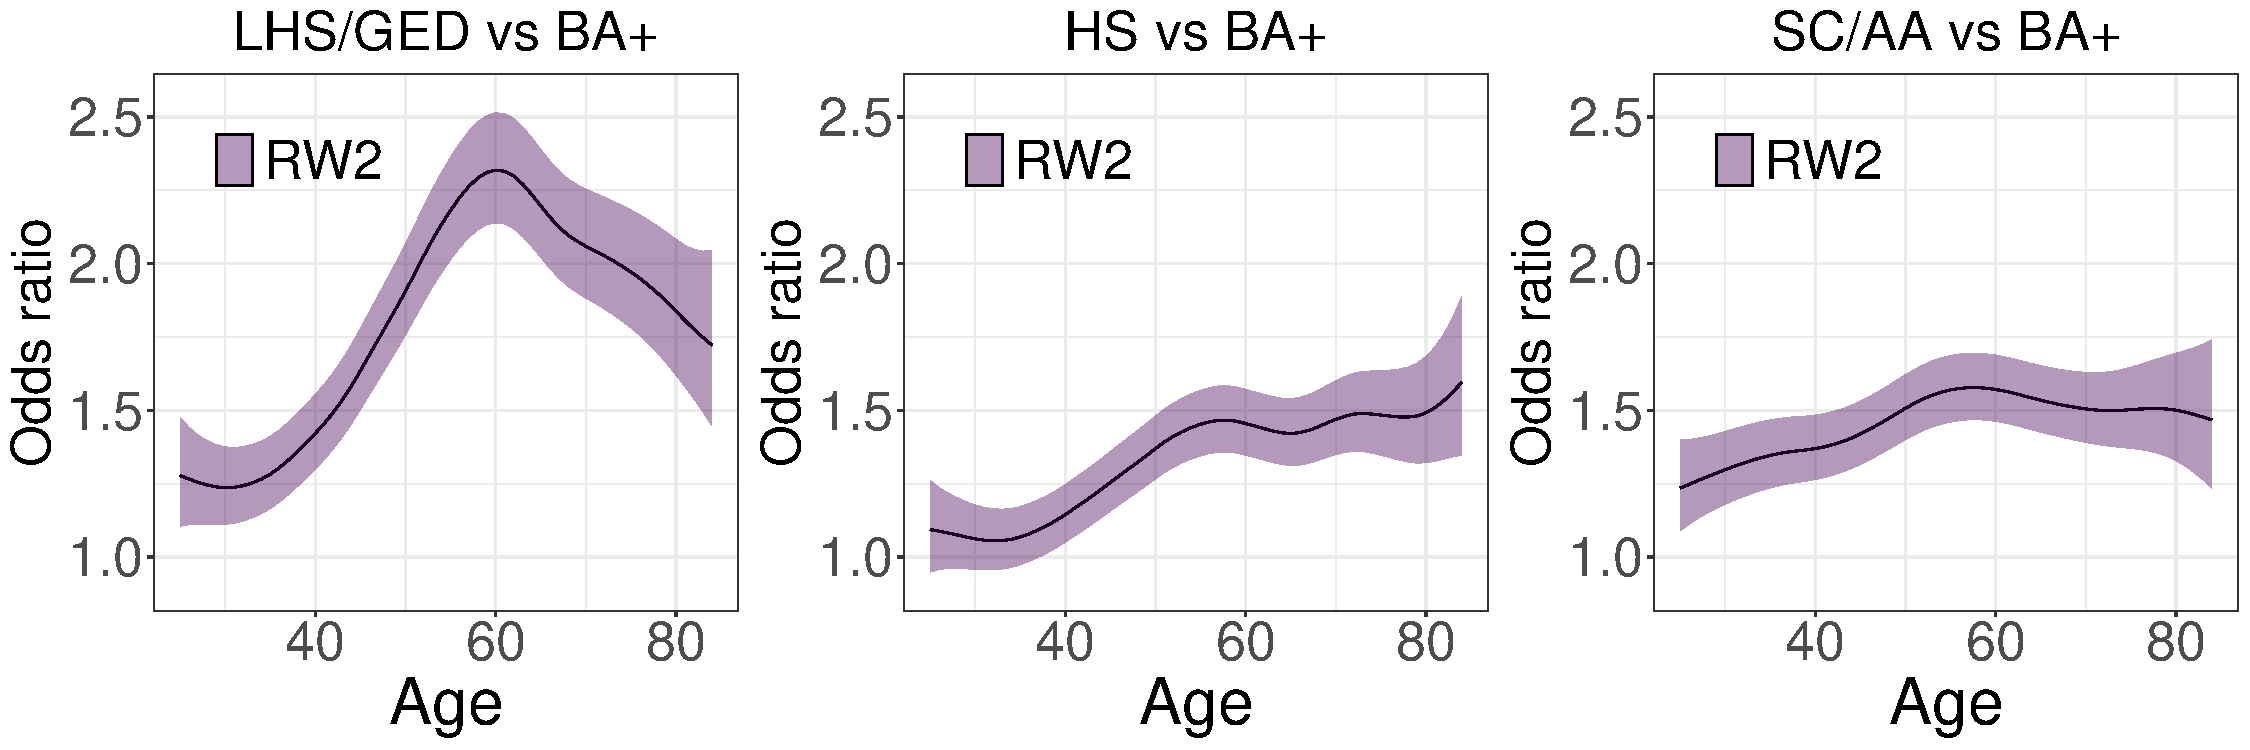
\includegraphics[width=\textwidth]{Figures/rw2_age_f.pdf}
    \end{subfigure}
    \vskip\baselineskip\vspace{-0.3cm}
    \begin{subfigure}[b]{\textwidth}   
        \centering 
        \caption[]%
        {}    
        \label{figure:Application1:rw2_cohort_f}
        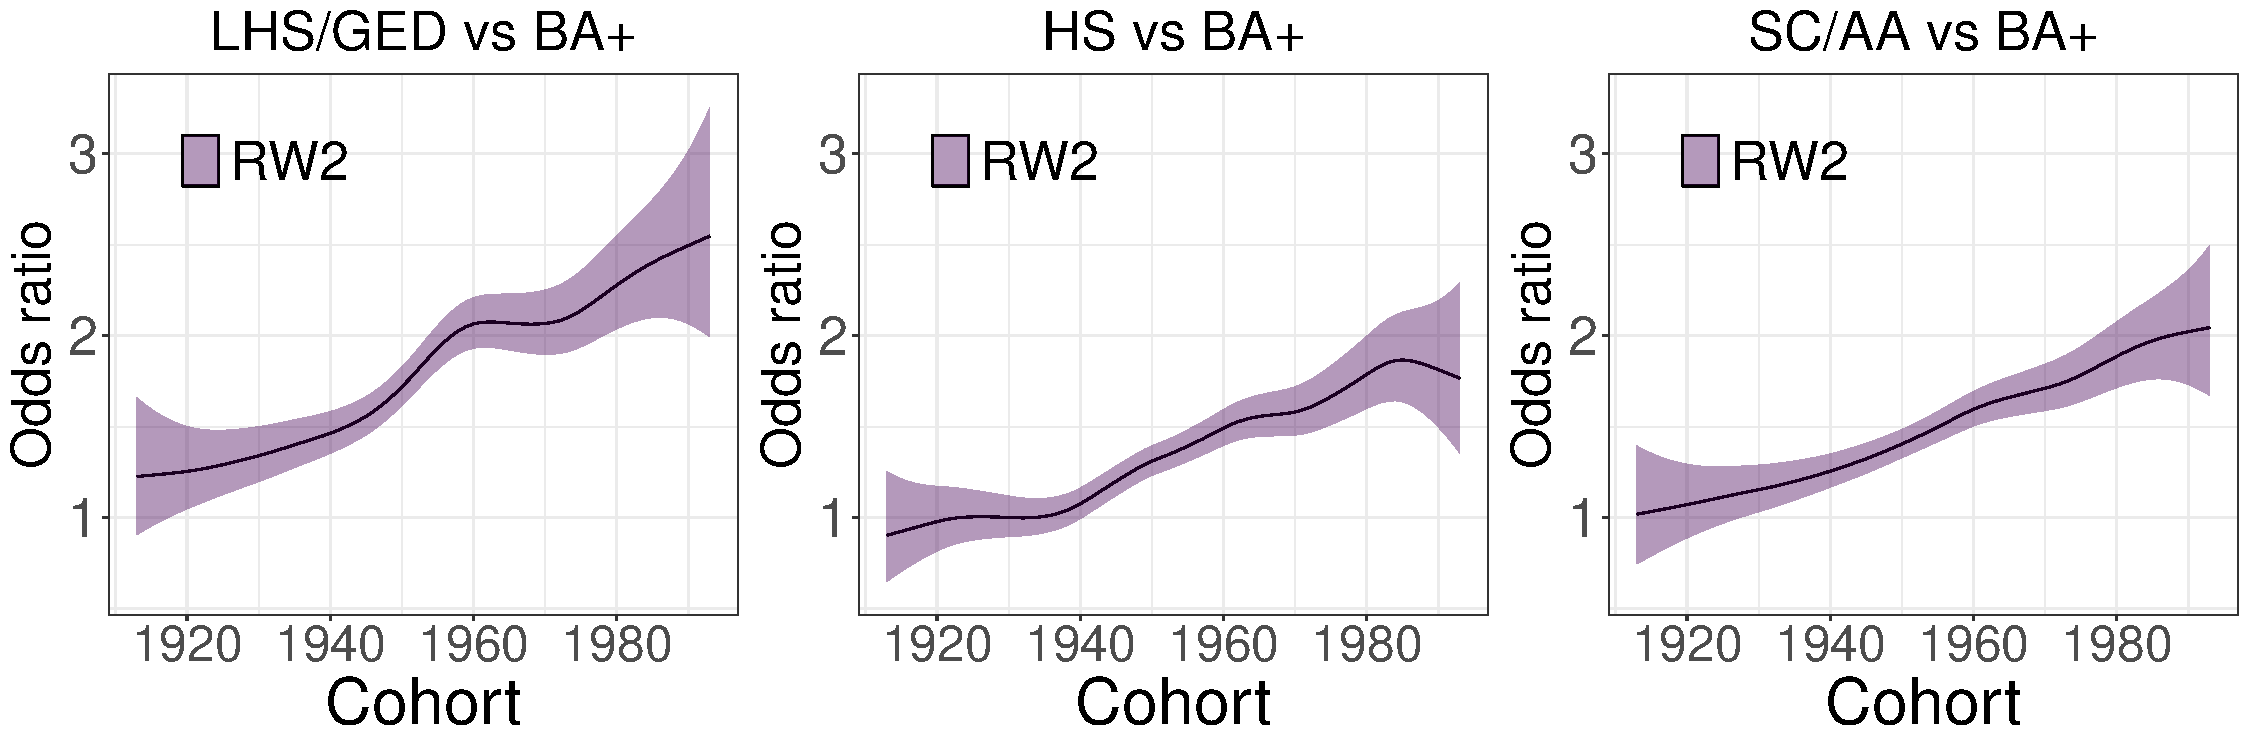
\includegraphics[width=\textwidth]{Figures/rw2_cohort_f.pdf}
    \end{subfigure}
    \caption{The posterior estimated median odds-ratio over (a) age and (b) cohort, for different levels of attained education with respect to the highest level of education, along with a $95\%$ credible interval for an aPc model, using female data and RW2 priors for each temporal component in the latent field. A PC$(10,0.01)$ prior is placed on the standard deviation of each component.}
    \label{figure:Application1:rw2_f}
\end{figure}

\captionsetup[subfigure]{labelfont={bf,large}, font={large}, skip=1pt, margin=0cm, singlelinecheck=true}

%Compare standard deviation plot for male data
\begin{figure}[h!]
    \centering
    \includegraphics[width=0.8\textwidth]{Figures/compare_plots_s0_m.pdf}
    \caption{The prior (left) and posterior (right) distributions of the standard deviation in aPc models using male data along with expert knowledge (EK), anti-EK, Dirichlet, and component-specific (CS) priors outlined in Section \ref{section:application1:prior}. }
    \label{figure:Application1:s0_m}
\end{figure}

%Compare posterior plots for male data
\begin{figure}[h]
    \centering
    \begin{subfigure}[b]{0.8\textwidth}
        \centering
        \includegraphics[width=\textwidth]{Figures/compare_plots_s1_m.pdf}
        \caption[Network2]%
        {{\small Top split}}    
        \label{figure:Application1:s1_m}
    \end{subfigure}
    \vskip\baselineskip\vspace{-0.5cm}
    \begin{subfigure}[b]{0.8\textwidth}   
        \centering 
        \includegraphics[width=\textwidth]{Figures/compare_plots_s2_m.pdf}
        \caption[]%
        {{\small Middle split}}    
        \label{figure:Application1:s2_m}
    \end{subfigure}
    \vskip\baselineskip\vspace{-0.5cm}
    \begin{subfigure}[b]{0.8\textwidth}   
        \centering 
        \includegraphics[width=\textwidth]{Figures/compare_plots_s3_m.pdf}
        \caption[]%
        {{\small  Bottom split}}    
        \label{figure:Application1:s3_m}
    \end{subfigure}
    \vspace{-0.2cm}
    \caption{The prior (left) and posterior (right) distribution of the mixing parameters at different levels in the hierarchical structure of the EK prior in aPc models using male data, and the expert knowledge (EK), anti-EK, Dirichlet, and component-specific (CS) priors outlined in Section \ref{section:application1:prior}. }
    \label{figure:Application1:compare-plots_m}

\end{figure}

\FloatBarrier
\subsubsection{Details on implementation in \texttt{R}}
\label{appendix:implementation:prior}
The \texttt{R} package \texttt{makemyprior} allows us to implement the desired hierarchical decomposition priors with the desired shrinkage, as outlined in Section \ref{section:application1:priorspecification}, although some additional modifications to the integration between \texttt{makemyprior} and \texttt{INLA} had to be made in order to implement the desired structure of the EK prior. Below follows an explanation of the procedure.

%What measures was taken differently
As mentioned in Section \ref{section:application1:priorspecification}, due to the stratification by education, the stratum specific effects inherently require an additional weight parameter to split the variance between each stratum. This property is undesirable as it requires incorporation of prior beliefs on how the different strata explain the variance. The provided EK does not provide intuition on how this split should be made, and it is therefore desirable to perform computations on the levels in which EK is provided. As such, the resolution done here is to have the computational software compute at this level by providing priors and evaluation functions that facilitate this. To achieve this, the prior made in \texttt{makemyprior} has to recognize only one node for each stratum specific effect, and for the computed precision (inverse variance) of the four stratified random effects to be evaluated jointly in \texttt{INLA}. 

In \texttt{makemyprior}, random effects are specified in R-formula syntax using the \texttt{mc()} function which has similar functionality to the function \texttt{f()} found in \texttt{INLA}. For each of the age, period and cohort effects, the desired latent RW1 prior structure is specified using the option \texttt{model = "rw1"}. This way, stratum specific effects require four RW1 specifications, though for the sake of the prior we wish to have a single specification. To circumvent this, a user specified precision structure matrix is created using the Kronecker product with the $4\times 4$ identity matrix and the RW1 structure matrix shown in Equation \eqref{eqn:rw1-structure-matrix}. This matrix then contains the structure matrix for four independent RW1 effects, one for each of the four strata, modelled as one matrix. This matrix may then be used in a joint prior specification with a single precision as desired. The next step is to transform the indices from the four set of indices to run over the newly constructed matrix. As all of these sets of indices are of the same length, we consequently rearrange the indices to be $i'=i + e\cdot I$, where $e=1,2,3,4$ denotes the education level. Doing this for all the stratum specific effects, the random effect is modelled with the option \texttt{model = "generic0"} while supplying the new structure matrix as the \texttt{Cmatrix}. As a consequence, the stratum specific effect is evaluated as one effect in the prior. 

Next, \texttt{INLA} has to evaluate the four random effects generated by the stratification of a random effect as a single random effect, as the prior constructed with \texttt{makemyprior} suggests. To do this, the formula supplied to \texttt{INLA} will not use the matrix constructed above, but is provided a random effect for each stratum of a stratum specific effect. Using expert settings in \texttt{INLA}, we may supply \texttt{INLA} variations of the functions normally passed on by \texttt{makemyprior} to make sense of the joint prior specifications generated by \texttt{makemyprior}. To achieve the desired result, the precision evaluation function is modified to pool the precision of the random effects before computations, meaning the computations are preformed on the parent node level, and not at the leaf node level. In \texttt{INLA}, the precisions of the random effects are given as log-precisions, meaning that the pooling is achieved by transforming to precisions, summing them, and then transforming back to log-precisions. 

\FloatBarrier
\subsubsection{Linear combinations in \texttt{INLA}}
\label{appendix:implementation:lincombs}
A full example of how the linear combinations are specified in \texttt{R} using \texttt{INLA} with toy-data is included in the Github repository of the thesis (\href{https://github.com/Markutr/Masteroppgave}{https://github.com/Markutr/Masteroppgave}). Here, we give some a high-level overview of how it is done.

In \texttt{INLA}, a linear combination of random and fixed effects are specified using the function \texttt{inla.make.lincomb()}. Let us consider a simple case with three age groups, three periods and two education levels. We let $i$ $(i= 1,2,3)$ denote the age groups, $j$ $(j= 1,2,3)$ denote the periods, $k$ $(k= 1,2,3,4,5)$ denote the cohorts, and $e$ $(e= 1,2)$ denote the level of education. Moreover, we consider an aPC model, where the age effect is education-specific and the period and cohort effects are shared between stratum. We let $\mu_e$ denote the education-specific intercept, $\theta_{ie}$ denote the age effect, $\phi_j$ denote the period effect, $\psi_k$ denote the cohort effect and $\varepsilon_{ije}$ denote an unstructured effect. Finally, we model the probabilities $\pi_{ije}$ on a logit scale. The linear predictor (akin to Equation \eqref{eqn:linear-pred}) defining the model is then
\begin{equation}
    \text{logit}(\pi_{ije}) = \mu_e + \theta_{ie} + \phi_j + \psi_k + \varepsilon_{ije}.
\end{equation}
In our example here, we will be basing our explanation using the model specified in the \texttt{R} formula syntax:
\begin{lstlisting}
    formula = -1 + Education1 + Education2 + 
              f(Age_Education1, model = "rw1") + 
              f(Age_Education2, model = "rw1") +
              f(Period, model = "rw1") +
              f(Cohort, model = "rw1") +
              f(eps, model = "iid")
\end{lstlisting}
That is, the education-specific age effect is modelled as two separate random effects. 

\subsubsubsection*{Fixed effects}
In code, if the education-specific intercepts for the two education levels are given as "Education1" and "Education2" in the formula syntax, then we may specify a linear combination of their difference as
\begin{lstlisting}
    inla.make.lincomb(Education1 = 1, 
                      Education2 = -1)
\end{lstlisting}
Note that this corresponds to $\mu_1 - \mu_2$. If we wanted different coefficients (say $2\mu_1 - 0.1\mu_2$), then change the respective number in the function call. 

\subsubsubsection*{Random effects}
When passing data to \texttt{INLA}, each random effect is described over a set of indices. In our example, theses are provided in the given formula as "Age\_Education1", "Age\_Education2", "Period", "Cohort" and "eps". For each effect we wish to include in a linear combination, the \texttt{inla.make.lincomb()} function takes an array the length of this set of indices. The array is provided as a named argument with the same name as the set of indices it corresponds to. In this array, the random effect at the given position corresponds to random effect described at that position in the given indices. To omit effects, provide NA at the corresponding array positions. To include effects, provide the coefficient of the effect in the desired linear combination. For instance, say we wish to specify the linear combination describing the difference in the age effects between the strata for age group 2. Then, the formula is
\begin{lstlisting}
    inla.make.lincomb(Age_Education1 = c(NA,1,NA), 
                      Age_Education2 = c(NA, -1, NA))
\end{lstlisting}

\subsubsubsection*{Both fixed and random effects}
Linear combinations may be specified using both fixed and random effects at the same time (as done in our application). To do this, simply include the fixed and random effects as before. That is, 
\begin{lstlisting}
    inla.make.lincomb(Age_Education1 = c(NA,1,NA),
                      Age_Education2 = c(NA,-1,NA),
                      Education1 = 1,
                      Education2 = -1)
\end{lstlisting}


\subsubsection{Individual specific MAPC model}
\label{appendix:individual}
As argued in Section \ref{section:Application1}, the granularity of which we consider our analysis should not matter for anything other than computational time, as it is aggregated in \texttt{INLA}. To show this, a model was also fitted on the individual level data using the EK-prior derived in Section \ref{section:application1:prior}. Figure \ref{figure:Application2:lincombs_f_ind} shows the posterior median odds-ratio over age and cohorts in the aPc model using individual level data. The model using aggregated data (as in \ref{section:application1:results}) is also included to show that they are identical. Moreover, Figure \ref{figure:INDI:s0_f} shows the posterior distribution of the total variance $\sigma^2$ along with the prior, showing nearly identical posteriors for both models. Figure \ref{figure:INDI:compare-plots_f} shows the posterior distribution of the mixing parameters $\omega_{\text{top}}$, $\omega_{\text{mid}}$ and $\omega_{\text{bot}}$ (as described in \ref{section:application1:priorspecification}) based on $10,000$ samples, at each split of the prior tree structure used to formulate the EK-Prior. From these figures it is clear that the models provide the same fit, and for practical purposes are the same. Individual-specific covariates are therefore straightforward to include in future research.

\captionsetup[subfigure]{labelfont={bf,large}, font={large}, skip=1pt, margin=0cm, singlelinecheck=false}
\begin{figure}[h!]
    \centering
    \begin{subfigure}[b]{\textwidth}   
        \centering 
        \caption[]%
        {}    
        \label{figure:Application2:age_diff_f_ind}
        \includegraphics[width=\textwidth]{Figures/lincomb_ind_agg_m_age.pdf}
    \end{subfigure}
    \vskip\baselineskip\vspace{-0.3cm}
    \begin{subfigure}[b]{\textwidth}   
        \centering 
        \caption[]%
        {}    
        \label{figure:Application2:cohort_diff_f_ind}
        \includegraphics[width=\textwidth]{Figures/lincomb_ind_agg_m_cohort.pdf}
    \end{subfigure}
    \vspace{-0.2cm}
    \caption{The estimated difference in (a) age effects and (b) cohort effects between education levels along with a $95\%$ credible interval, all with respect to education attained at level bachelor or higher for the models using the data in an individual-specific and aggregated form.}
    \label{figure:Application2:lincombs_f_ind}
\end{figure}

\captionsetup[subfigure]{labelfont={bf,large}, font={large}, skip=1pt, margin=0cm, singlelinecheck=true}
%INDIVIDIAL S0
\begin{figure}[h!]
    \centering
    \includegraphics[width=0.8\textwidth]{Figures/compare_plots_indi_s0_f.pdf}
    \caption{The prior (left) and posterior (right) distributions of the standard deviation in aPc models using female data along with the expert knowledge (EK), anti-EK, and Dirichlet priors outlined in Section \ref{section:application1:prior}. The posterior when using the data on an individual-specific format is also included, labelled as "Individual", and uses the EK prior.}
    \label{figure:INDI:s0_f}
\end{figure}

%INDIVIDUAL SPLITS
\begin{figure}[h]
    \centering
    \begin{subfigure}[b]{0.8\textwidth}
        \centering
        \includegraphics[width=\textwidth]{Figures/compare_plots_indi_s1_f.pdf}
        \caption[Network2]%
        {{\small Top split}}    
        \label{figure:INDI:s1_f}
    \end{subfigure}
    \vskip\baselineskip\vspace{-0.5cm}
    \begin{subfigure}[b]{0.8\textwidth}   
        \centering 
        \includegraphics[width=\textwidth]{Figures/compare_plots_indi_s2_f.pdf}
        \caption[]%
        {{\small Middle split}}    
        \label{figure:INDI:s2_f}
    \end{subfigure}
    \vskip\baselineskip\vspace{-0.5cm}
    \begin{subfigure}[b]{0.8\textwidth}   
        \centering 
        \includegraphics[width=\textwidth]{Figures/compare_plots_indi_s3_f.pdf}
        \caption[]%
        {{\small  Bottom split}}    
        \label{figure:INDI:s3_f}
    \end{subfigure}
    \vspace{-0.2cm}
    \caption{The prior (left) and posterior (right) distribution of the mixing parameters at different levels in the hierarchical structure of the EK prior in aPc models using female data and the expert knowledge (EK), anti-EK, and Dirichlet priors outlined in Section \ref{section:application1:prior}. The posteriors when using the data on an individual-specific format are also included, labelled as "Individual", and uses the EK prior.}
    \label{figure:INDI:compare-plots_f}
\end{figure}

\FloatBarrier
\subsection{Extras of Section \ref{section:application2}}
\label{appendix:application2}
\subsubsection{Extra figures}


\captionsetup[subfigure]{labelfont={bf,large}, font={large}, skip=1pt, margin=0cm, singlelinecheck=false}
\begin{figure}[h!]
    \centering
    \begin{subfigure}[b]{\textwidth}   
        \centering 
        \caption[]%
        {}    
        \label{figure:Application1:rw2_age_f_fil}
        \includegraphics[width=\textwidth]{Figures/lincomb_survey_filtered_age_f_rw2.pdf}
    \end{subfigure}
    \vskip\baselineskip\vspace{-0.3cm}
    \begin{subfigure}[b]{\textwidth}   
        \centering 
        \caption[]%
        {}    
        \label{figure:Application1:rw2_cohort_f_fil}
        \includegraphics[width=\textwidth]{Figures/lincomb_survey_filtered_cohort_f_rw2.pdf}
    \end{subfigure}
    \caption{The posterior estimated median odds-ratio over \textbf{(a)} age and \textbf{(b)} cohort, for different levels of attained education with respect to the highest level of education along with $95\%$ credible intervals. The trends are shown for two latent field priors (RW1 and RW2) placed on each temporal component in the latent field. A PC$(10,0.01)$ prior is placed on the standard deviation of each component in the RW2 prior, and the EK prior was used in the model with RW1 priors on the latent field. In these aPc models, data from the female, white, U.S-born population was used, and the complex survey design was accounted for. }
    \label{figure:Application1:rw2_f_fil}
\end{figure}

\begin{figure}[h!]
    \centering
    \begin{subfigure}[b]{\textwidth}   
        \centering 
        \caption[]%
        {}    
        \label{figure:Application1:rw2_age_m_fil}
        \includegraphics[width=\textwidth]{Figures/lincomb_survey_filtered_age_m_rw2.pdf}
    \end{subfigure}
    \vskip\baselineskip\vspace{-0.3cm}
    \begin{subfigure}[b]{\textwidth}   
        \centering 
        \caption[]%
        {}    
        \label{figure:Application1:rw2_cohort_m_fil}
        \includegraphics[width=\textwidth]{Figures/lincomb_survey_filtered_cohort_m_rw2.pdf}
    \end{subfigure}
    \caption{The posterior estimated median odds-ratio over \textbf{(a)} age and \textbf{(b)} cohort, for different levels of attained education with respect to the highest level of education along with $95\%$ credible intervals. The trends are shown for two latent field priors (RW1 and RW2) placed on each temporal component in the latent field. A PC$(10,0.01)$ prior is placed on the standard deviation of each component in the RW2 prior, and the EK prior was used in the model with RW1 priors on the latent field. In these aPc models, data from the male, white, U.S-born population was used, and the complex survey design was accounted for. }
    \label{figure:Application1:rw2_m_fil}
\end{figure}

\FloatBarrier
\subsubsection{Details on implementation in \texttt{R}}
\label{appendix:A2:implementaion}
To obtain the estimated probabilities at the logit scale along with estimates of the variance, the \texttt{survey} package in \texttt{R} was used. The package takes the data on an individual specific level and computes estimates of $\pi_{ije}$ and $\sigma^2_{ije}$ for each stratum according to the provided strata using the provided weights. In \texttt{R}, the survey design is specified by
\begin{lstlisting}
des<-svydesign(ids= ~1, strata= ~age+period+education,
                 weights=~sampweight, data = data)
\end{lstlisting}
where the strata denotes the indices $i$, $j$ and $e$ as age, period and education, and the sample weights are provided as \texttt{sampweight} in the data object. The argument \texttt{ids=~1} is required to specify that there are no clusters in the data to correct for. The estimates are then obtained by
\begin{lstlisting}
prevs=svyby(~backpain, 
            by=~education+age+period,
            design=des, FUN=svymean)
\end{lstlisting}
The weighted sample estimators are then transformed by the logit function in Equation \eqref{eqn:logit}, and the variance in Equation \eqref{eqn:asymptoticDistribution} is computed from the weighted sample estimator and the standard deviance estimates. 

To fix the variances, the precision of the latent field was set to $1$ for all observations by supplying \texttt{INLA} with the option \texttt{control.family = list(hyper = list(prec = list(initial = log(1), fixed = T)))}, and then scaled by the transformed precisions using the \texttt{scale} option in the INLA call.

\begin{lstlisting}
    result = inla(formula = your_formula, 
                  data = your_data, 
                  family = "gaussian", 
                  control.family = list(
                    hyper=list(
                      prec=list(
                        initial = log(1), fixed = T))),
                  scale = scale)
\end{lstlisting}








% Indeks for rapporten. Ta bort prosenttegn hvis du vil ha det med.
%\printindex

% Avslutter dokumentet vårt:
\end{document}

% Local Variables:
% TeX-master: "master"
% End:
